% Esta es la Plantilla UNAL en LaTeX
\documentclass[12pt,spanish,openany,twoside,letterpaper]{book}

\usepackage[nottoc]{tocbibind} %------bibliografía------%
\usepackage{notoccite}

%Idioma del documento
%Use main para el idioma principal del documento
\usepackage[main=spanish,british,ngerman]{babel}
\decimalpoint

\usepackage[utf8]{inputenc} % allow utf-8 input
\usepackage[T1]{fontenc}    % Caracteres especiales

% Evita ligadura li & fl
\usepackage{microtype}
\DisableLigatures{encoding = *, family = *}

\usepackage{lipsum}
\usepackage{gensymb}

% Otros paquetes de tablas y colores avanzados
\usepackage{siunitx} %------unidades------%
\usepackage{graphicx,float,multirow,multicol}
\graphicspath{{./figures/}}
\usepackage{caption, subcaption}
\DeclareCaptionSubType[alph]{figure}
\captionsetup[subfigure]{labelformat=simple,justification=centerlast}
\renewcommand\thesubfigure{(\alph{subfigure})}
\makeatletter
\renewcommand\p@subfigure{\thefigure}
\makeatother
\usepackage{booktabs}
\usepackage{amsmath,amsfonts,amssymb,amstext,amsthm, xfp, latexsym}
% NUNCA INCLUIR EL PAQUETE "mathpazo"
\usepackage{bm} % bold math expressions $\bm{expression}$
\usepackage{cancel}
\usepackage{longtable}
\setlength{\LTcapwidth}{6in}

\usepackage[dvipsnames]{xcolor}
\usepackage{listings}
\definecolor{codegreen}{rgb}{0,0.6,0}
\definecolor{codegray}{rgb}{0.5,0.5,0.5}
\definecolor{codepurple}{rgb}{0.58,0,0.82}
\definecolor{backcolour}{rgb}{0.95,0.95,0.92}

\lstdefinestyle{mystyle}{
    backgroundcolor=\color{backcolour},   
    commentstyle=\color{codegreen},
    keywordstyle=\color{magenta},
    numberstyle=\tiny\color{codegray},
    stringstyle=\color{codepurple},
    basicstyle=\ttfamily\footnotesize,
    breakatwhitespace=false,         
    breaklines=true,                 
    captionpos=b,                    
    keepspaces=true,                 
    numbers=left,                    
    numbersep=5pt,                  
    showspaces=false,                
    showstringspaces=false,
    showtabs=false,                  
    tabsize=1
}

\lstset{style=mystyle}

%\usepackage[autostyle, english=british]{csquotes}
%\MakeOuterQuote{"}

\usepackage{epsfig,epic,eepic,threeparttable,amscd,here,lscape,tabularx}
\usepackage{textcomp}
\usepackage{tabu,array}

% Permite ver y configurar los parámetros de la página
\usepackage{layout}
%Hyperref permite ver las secciones del texto
\usepackage[hidelinks]{hyperref}
\hypersetup{
    colorlinks=true,
    linkcolor=blue,
    filecolor=magenta,      
    urlcolor=blue,
    citecolor=blue,
}
\usepackage{cleveref} %cleveref has to be added after hyperref

%Permite incluir código de cualquier lenguaje dentro del texto del documento
% \usepackage{minted}
\usepackage{fancyvrb}
\newenvironment{myverbatim}{\Verbatim}{\endVerbatim}

\crefrangelabelformat{subsection}{#3#1#4-#5\crefstripprefix{#1}{#2}#6}

%Genera los comandos de la página de autoría
\newcommand{\studentname}{}
\newcommand{\submissiondate}{}
\newcommand{\academictitle}{}
\newcommand{\resgroupone}{}
\newcommand{\resgrouptwo}{}
\newcommand{\researchtopic}{}
\newcommand{\thesisname}{}
\newcommand{\director}{}
\newcommand{\codirector}{}
\newcommand{\issuedate}{}
\newcommand{\palabrasclave}{}
\newcommand{\keywords}{}
\newcommand{\schlusselworter}{}
\newcommand{\palavraschave}{}
\newcommand{\sede}{}
\newcommand{\department}{}
\newcommand{\faculty}{}

%Información de la tesis
%Diligenciar aquí los datos para su carga automática donde se requiera en el documento
\renewcommand{\studentname}{Andrés Felipe Vargas-Londoño}
\renewcommand{\thesisname}{CosmicWatch: The Desktop Muon Detectors, exploring gamma-ray spectroscopy}
\renewcommand{\issuedate}{2024}
\renewcommand{\submissiondate}{Fecha entrega}
\renewcommand{\director}{Prof. Luis Fernando Cristancho Mejia}
\renewcommand{\codirector}{Prof. Spencer Axani}
\renewcommand{\academictitle}{Físico}
\renewcommand{\resgroupone}{Grupo de Física Nuclear Universidad Nacional (GFNUN)}
\renewcommand{\resgrouptwo}{Axani Group (AxLab)}
\renewcommand{\researchtopic}{Espectroscopía gamma}
\renewcommand{\sede}{Sede Bogotá} 
\renewcommand{\department}{Departamento de Física}
\renewcommand{\faculty}{Facultad de Ciencias}

%Palabras clave del documento - Tener presente los Theasurus https://www.thesaurus.com/
%Disponible en 3 idiomas aunque se puede extender a francés o otro idioma
\renewcommand{\palabrasclave}{CosmicWatch, RaspberryPi Pico, Radiación gamma, Centelleo.}
\renewcommand{\keywords}{CosmicWatch, RaspberryPi Pico, Gamma radiation, Scintillation.}
%\renewcommand{\schlusselworter}{}
%\renewcommand{\palavraschave}{}

\usepackage{footnote}
\makesavenoteenv{tabular}
%Formatting for headers and footers
\usepackage{fancyhdr}
\pagestyle{fancy}

\fancypagestyle{plain}

\newcommand{\RomanNumeralCaps}[1]
    {\MakeUppercase{\romannumeral #1}}

%\fancyhead[RO,LE]{Monolithic Nanocomposite Detector for LaBrAT-PET}

% Redefinir \sectionmark
\renewcommand{\sectionmark}[1]{\markright{#1}}
% Redefinir \leftmark para mostrar solo el nombre de la sección
\renewcommand{\chaptermark}[1]{\markboth{#1}{}}

% Configurar encabezado y pie de página
\fancyhead[L]{\fontsize{10}{12} \selectfont Personal Statement}
\fancyhead[RO]{\fontsize{10}{12} \selectfont \thepage} % Encabezado derecho en páginas impares
\fancyhead[LO]{\fontsize{10}{12} \selectfont \textbf{\leftmark}}   % Encabezado izquierdo en páginas impares
\fancyhead[RE]{\fontsize{10}{12} \selectfont \textbf{\thesisname}}   % Encabezado izquierdo en páginas pares
\fancyhead[LE]{\fontsize{10}{12} \selectfont \thepage}  % Encabezado derecho en páginas pares
\fancyfoot[C]{}            % Pie de página central vacío

\usepackage{titlesec}
% Permite personalizar los títulos de sección y de capítulos
% hang lo deja en el mismo renglón, display lo despliega
% Elimina el "Capitulo" y deja solo el número
\titleformat{\chapter}[hang]
  {\Huge\bfseries}{\thechapter}{0.5cm}{\Huge}
%\titleformat{\section}[hang]{\sffamily\LARGE}{\thesection}{0.5cm}{}
%\titleformat{\subsection}[hang]{\sffamily\Large}{\thesubsection}{0.5cm}{}
%\titleformat{\subsubsection}[hang]{\sffamily\large}{\thesubsubsection}{0.5cm}{}
%\titleformat{\paragraph}[runin]{\sffamily\normalsize}{}{}{\emph}

%Coloca anexo o apéndice en la Tabla de contenido
\usepackage[toc,page]{appendix}
% Configuración de las páginas en twoside-mode
% Permite ver y configurar los parámetros de la página
\setlength{\voffset}{-0.25in}
\setlength{\headwidth}{467pt}
\setlength{\headheight}{22pt}
\setlength{\oddsidemargin}{0pt}
\setlength{\evensidemargin}{0pt}
\setlength{\marginparwidth}{0pt}
\setlength{\marginparsep}{0pt}
\setlength{\parskip}{2em}
\setlength{\footskip}{20pt}
\setlength{\textheight}{650pt}
\setlength{\textwidth}{467pt}
\setlength{\headsep}{5pt}
\setlength{\parindent}{0pt}
\setlength{\baselineskip}{10pt plus 5pt minus 5pt}
\renewcommand{\theequation}{\thechapter-\arabic{equation}}
\renewcommand{\thefigure}{\textbf{\thechapter-\arabic{figure}}}
\renewcommand{\thetable}{\textbf{\thechapter-\arabic{table}}}


%Define la distancia de la primera linea de un párrafo a la margen
\parindent0cm 

%Espacio entre lineas
\renewcommand{\baselinestretch}{1}

%Para rotar texto, objetos y tablas seite.
%\usepackage{rotating}

%Permite incluir mecanismos y reacciones químicas
%\usepackage{tikz}
\usepackage{rotating}
\usepackage{circuitikz}
\usepackage{tikz-qtree}
%\usetikzlibrary{trees}
\usetikzlibrary{babel}
\usetikzlibrary{calc}
%\usepackage{chemformula}
%\usepackage{chemfig}

%\usetikzlibrary{calc,arrows.meta}% per right to e left to
%\tikzset{
%myedge/.style={->, -{Latex[#1]}}
%}

%Fuente de la presentación Ancizar Sans UNAL
%Para usar este compilado en Overleaf se debe usar el compilador XeLaTeX o LuaLaTeX!!
%Menu -> Compiler -> XeLaTeX o LuaLaTeX
%La siguiente línea debe comentarse si desea compilar con pdfLaTeX
%\RequireXeTeX


% Definición de la fuente Ancizar Sans
\newif\ifxetexorluatex

\ifxetexorluatex
  \usepackage{fontspec}
  \usefonttheme{serif}
  \setmainfont{AncizarSans}[Path=./AncizarSans/,Scale=1,Extension=.otf,UprightFont=*-Regular,BoldFont=*-Bold,ItalicFont=*-Italic,BoldItalicFont=*-BoldItalic]
\else
  % Si se compila con pdfLaTeX, cargar la fuente apropiada aquí
  \usepackage[T1]{fontenc}
\fi
% Metadatos del documento
\AtBeginDocument{%
	\hypersetup{
		pdfborder={0 0 0},
		pdfauthor={\studentname},
		pdfsubject={\thesisname}, 
		pdfcreator={\studentname},
		pdfproducer={\studentname},
	}
}

%Carga el símbolo de grado y el de Angstrom
\newcommand{\angstrom}{\textup{\AA}}
\newcommand{\grad}{$^{\circ}$}

%Inicio del documento, no olvide la etiqueta de cierre al final \end{document}
\begin{document}

%Nombres y formatos de títulos, tablas y figuras
%Use \sffamily para dejar con letra Sans Serif, sin etiqueta queda LaTeX clásico
\renewcommand{\listfigurename}{List of Figures}
\renewcommand{\listtablename}{List of Tables}
\renewcommand{\figurename}{Fig}
\renewcommand{\tablename}{Tab}
\renewcommand{\contentsname}{Table of contents}
\renewcommand{\chaptername}{Chapter}
%\renewcommand{\tablename}{\scriptsize \centering \textbf{Tabla}}
%\renewcommand{\figurename}{\scriptsize \centering \textbf{Figura}}
\renewcommand{\appendixname}{Appendix .}

%Cambia el nombre de la sección de referencias
\renewcommand{\bibname}{Bibliography}

\newcommand{\gps}{\texttt{gps}}

%Páginas de Presentación del documento - No modificar esto se hace automáticamente
{\newpage
\thispagestyle{empty}
\begin{center}
\begin{figure}
\centering

\epsfig{file=EscudoUN2016,scale=1}%
\end{figure}
\vspace{2.5cm}
\textbf{\Huge \thesisname} \\ 
\vspace{2.5cm}
\textbf{\Large \studentname} \\
\vspace{5.0cm}
\small Universidad Nacional de Colombia \\
\faculty \\
\department \\
\sede, Colombia\\
\issuedate
\newpage 
\thispagestyle{empty}
\vspace{2.5cm}
\textbf{\Huge \thesisname} \\
\vspace{2.5cm}
\textbf{\Large \studentname} \\
\vspace{2.5cm}
\small Tesis presentada como requisito parcial para optar por el título de: \\
{\bfseries \academictitle}\\
\vspace{2.5cm}
Director(a): \\
\director \\
Codirector(a): \\
\codirector \\
\vspace{2.5cm}
Línea de investigación: \\ 
\researchtopic\\
Grupo de investigación: \\
\resgroupone \\
\resgrouptwo \\
\vspace{2.0cm} 
Universidad Nacional de Colombia \\
\faculty \\
\department \\
\issuedate
\end{center}

% Dedicatorias
\newpage
\thispagestyle{empty}
\begin{flushright}
\begin{minipage}{12.5cm}
\noindent
\\[10em]
%Modificar la cita que se quiere agregar
{\Large Cita 01.}
\\[3em]
Autor
\\ \textit{Fuente}
\\[10em]
%Para anular la adición de una segunda cita anule las siguientes lineas desde acá mediante comentario (%)
%{\Large \textit{Wenn du es nicht einfach erkl\"{a}ren kannst, hast du es nicht genug verstanden} - Si no eres capaz de explicar algo claramente, es que aún no lo has entendido lo suficiente.}
\\[3em]
%Albert Einstein
%Hasta acá!
\end{minipage}
\end{flushright} 

% Declaración de originalidad del texto y del contenido
% No modificar, se hace automáticamente con los comandos ya definidos
\newpage
\chapter*{Declaración}\chaptermark{Declaración}
\par Me permito afirmar que he realizado ésta tesis de manera autónoma y con la única ayuda de los medios permitidos y no diferentes a los mencionados el presente texto. Todos los pasajes que se han tomado de manera textual o figurativa de textos publicados y no publicados, los he reconocido en el presente trabajo. Ninguna parte del presente trabajo se ha empleado en ningún otro tipo de tesis. 
\\[1em]
\sede., \submissiondate
\\[6em]
\rule{6cm}{0.5pt}\\
\studentname
}

%Páginas preámbulo, listado de figuras, tablas y tabla de contenido
{\pagestyle{plain} \pagenumbering{roman}
\setlength{\parskip}{1mm}
\chapter*{Acknowledgments}\chaptermark{Acknowledgments}
\addcontentsline{toc}{chapter}{Acknowledgments}%

This goes to my family, especially to my parents, for providing me with the most sincere and unconditional support I could have ever received. To every friend who stood there when things felt overwhelming and gave me the courage to keep going. Also to every professor and mentor who generously shared their knowledge and advice.
\\

A special thanks goes to Professor Fernando Cristancho for introducing me to an extremely nurturing working environment, filled with people without whom this could never have come to be. I am also deeply grateful to Professor Spencer N. Axani, for opening the doors to not only his group but also to immensely rewarding experiences and knowledge I will carry with me forever.
\\

Last but not least I want to thank me for believing in me, I want to thank me for doing all this hard work, for never quitting and for being me at all times.   
\chapter*{Listado de símbolos y abreviaturas}\chaptermark{Listado de símbolos y abreviaturas}
\addcontentsline{toc}{chapter}{Listado de símbolos y abreviaturas}
\newpage
\chapter*{Resumen}\chaptermark{Resumen}
\addcontentsline{toc}{chapter}{Resumen}%
\textbf{\Huge \ \strut CosmicWatch: Los Detectores de Muones de Escritorio, explorando la espectroscopia gamma \strut} %strut keeps interline spacing consistent
\vspace{.5cm}
\par El presente trabajo se concentra en el mejoramiento de CosmicWatch: Los Detectores de Escritorio de Muones, con el objetivo de obtener una resolución en energías suficiente para realizar espectroscopía gamma. Dadas ciertas limitaciones actuales en la electrónica, como tiempo muerto y baja rata de conteo, junto con la baja resolución de los centellatores plásticos usados hasta ahora, este trabajo explora entonces el uso de una RaspberryPi Pico y un cristal centellador basado en Lutecio y dopado con Cerio (LYSO:Ce), logrando resolución en energías de $13.5\%$ para 511 \unit{\kilo\eV} al medir con un osciloscopio Rohde\&Schwarz RTO6 y $28.3\%$ con modulos NIM.
\\[2cm]
\textbf{Palabras clave:} \palabrasclave

\newpage 
\chapter*{Abstract}\chaptermark{Abstract}
\addcontentsline{toc}{chapter}{Abstract}%
\textbf{\Huge \ \strut CosmicWatch: The Desktop Muon Detectors, exploring gamma-ray spectroscopy \strut} %strut keeps interline spacing consistent
\vspace{.5cm}
\par The present work focuses on the improvement of CosmicWatch: The Desktop Muon Detectors, with the goal of achieving sufficient energy resolution to allow for gamma spectroscopy. Due to current limitations in the electronics, such as dead time and small sample rate, in addition to the low energy resolution of previously used plastic scintillators, this work explores the use of a RaspberryPi Pico together with a Cerium-doped Lutetium-based scintillation crystal (LYSO:Ce), achieving energy resolutions of $13.5\%$ at 511 \unit{\kilo\eV} while sampling data with a Rohde\&Schwarz RTO6 oscilloscope and $28.3\%$ with NIM modules.
\\[2cm]
\textbf{Keywords:} \keywords

%\newpage 
%\chapter*{\sffamily Zusammenfassung}
%\addcontentsline{toc}{chapter}{Zusammenfassung}%
%\par Zusammenfassung texte.
%\par 
%\\[2cm]
%\textbf{Schlüsselwörter:} \schlusselworter
\tableofcontents 
%\addcontentsline{toc}{chapter}{Table of contents}
\listoffigures 
%\addcontentsline{toc}{chapter}{List of Figures}
\listoftables 
%\addcontentsline{toc}{chapter}{List of Tables}
\clearpage
}

{\pagenumbering{arabic}
\setlength{\parskip}{\baselineskip}
%Incluir secciones del documento de aquí en adelante
%Use \include para incluir desde una página nueva e \input para incluir sin salto de página
\include{chapters/introduction}
\chapter{Physical aspects}

\section{Radioactivity}

\section{Cosmic Radiation}

\section{Particle interactions with matter}
\chapter{Detector description}

%versions of the detector
\section{History}

``The desktop muon detector was initially built as a Muon Tagging Optical Modules (MTOMs) for PINGU, the proposed low energy upgrade for IceCube experiment'' \cite{CosmicWatch}. Since the first iteration, CosmicWatch has had multiple versions, always aiming to reduce size and costs, simplify its construction, and provide better documentation for new CosmicWatch users. An in-depth review of the detector evolution can be found in \cite{CosmicWatch} under ``About the project/Project evolution''.

The prototypes of CosmicWatch Fig. \ref{sfig:CW_ver1} used liquid scintillator, this however proved to be inefficient, since it was prone to leaks. The second prototype used a $5\times5\times5$ \unit{\cm\cubed} plastic scintillator in a light-tight reflective aluminum case Fig. \ref{sfig:CW_ver2}, this was however too slow, large, and expensive, making it not suitable for students.

\begin{figure}[H]
  \centering
  \begin{subfigure}[t]{0.45\textwidth}
    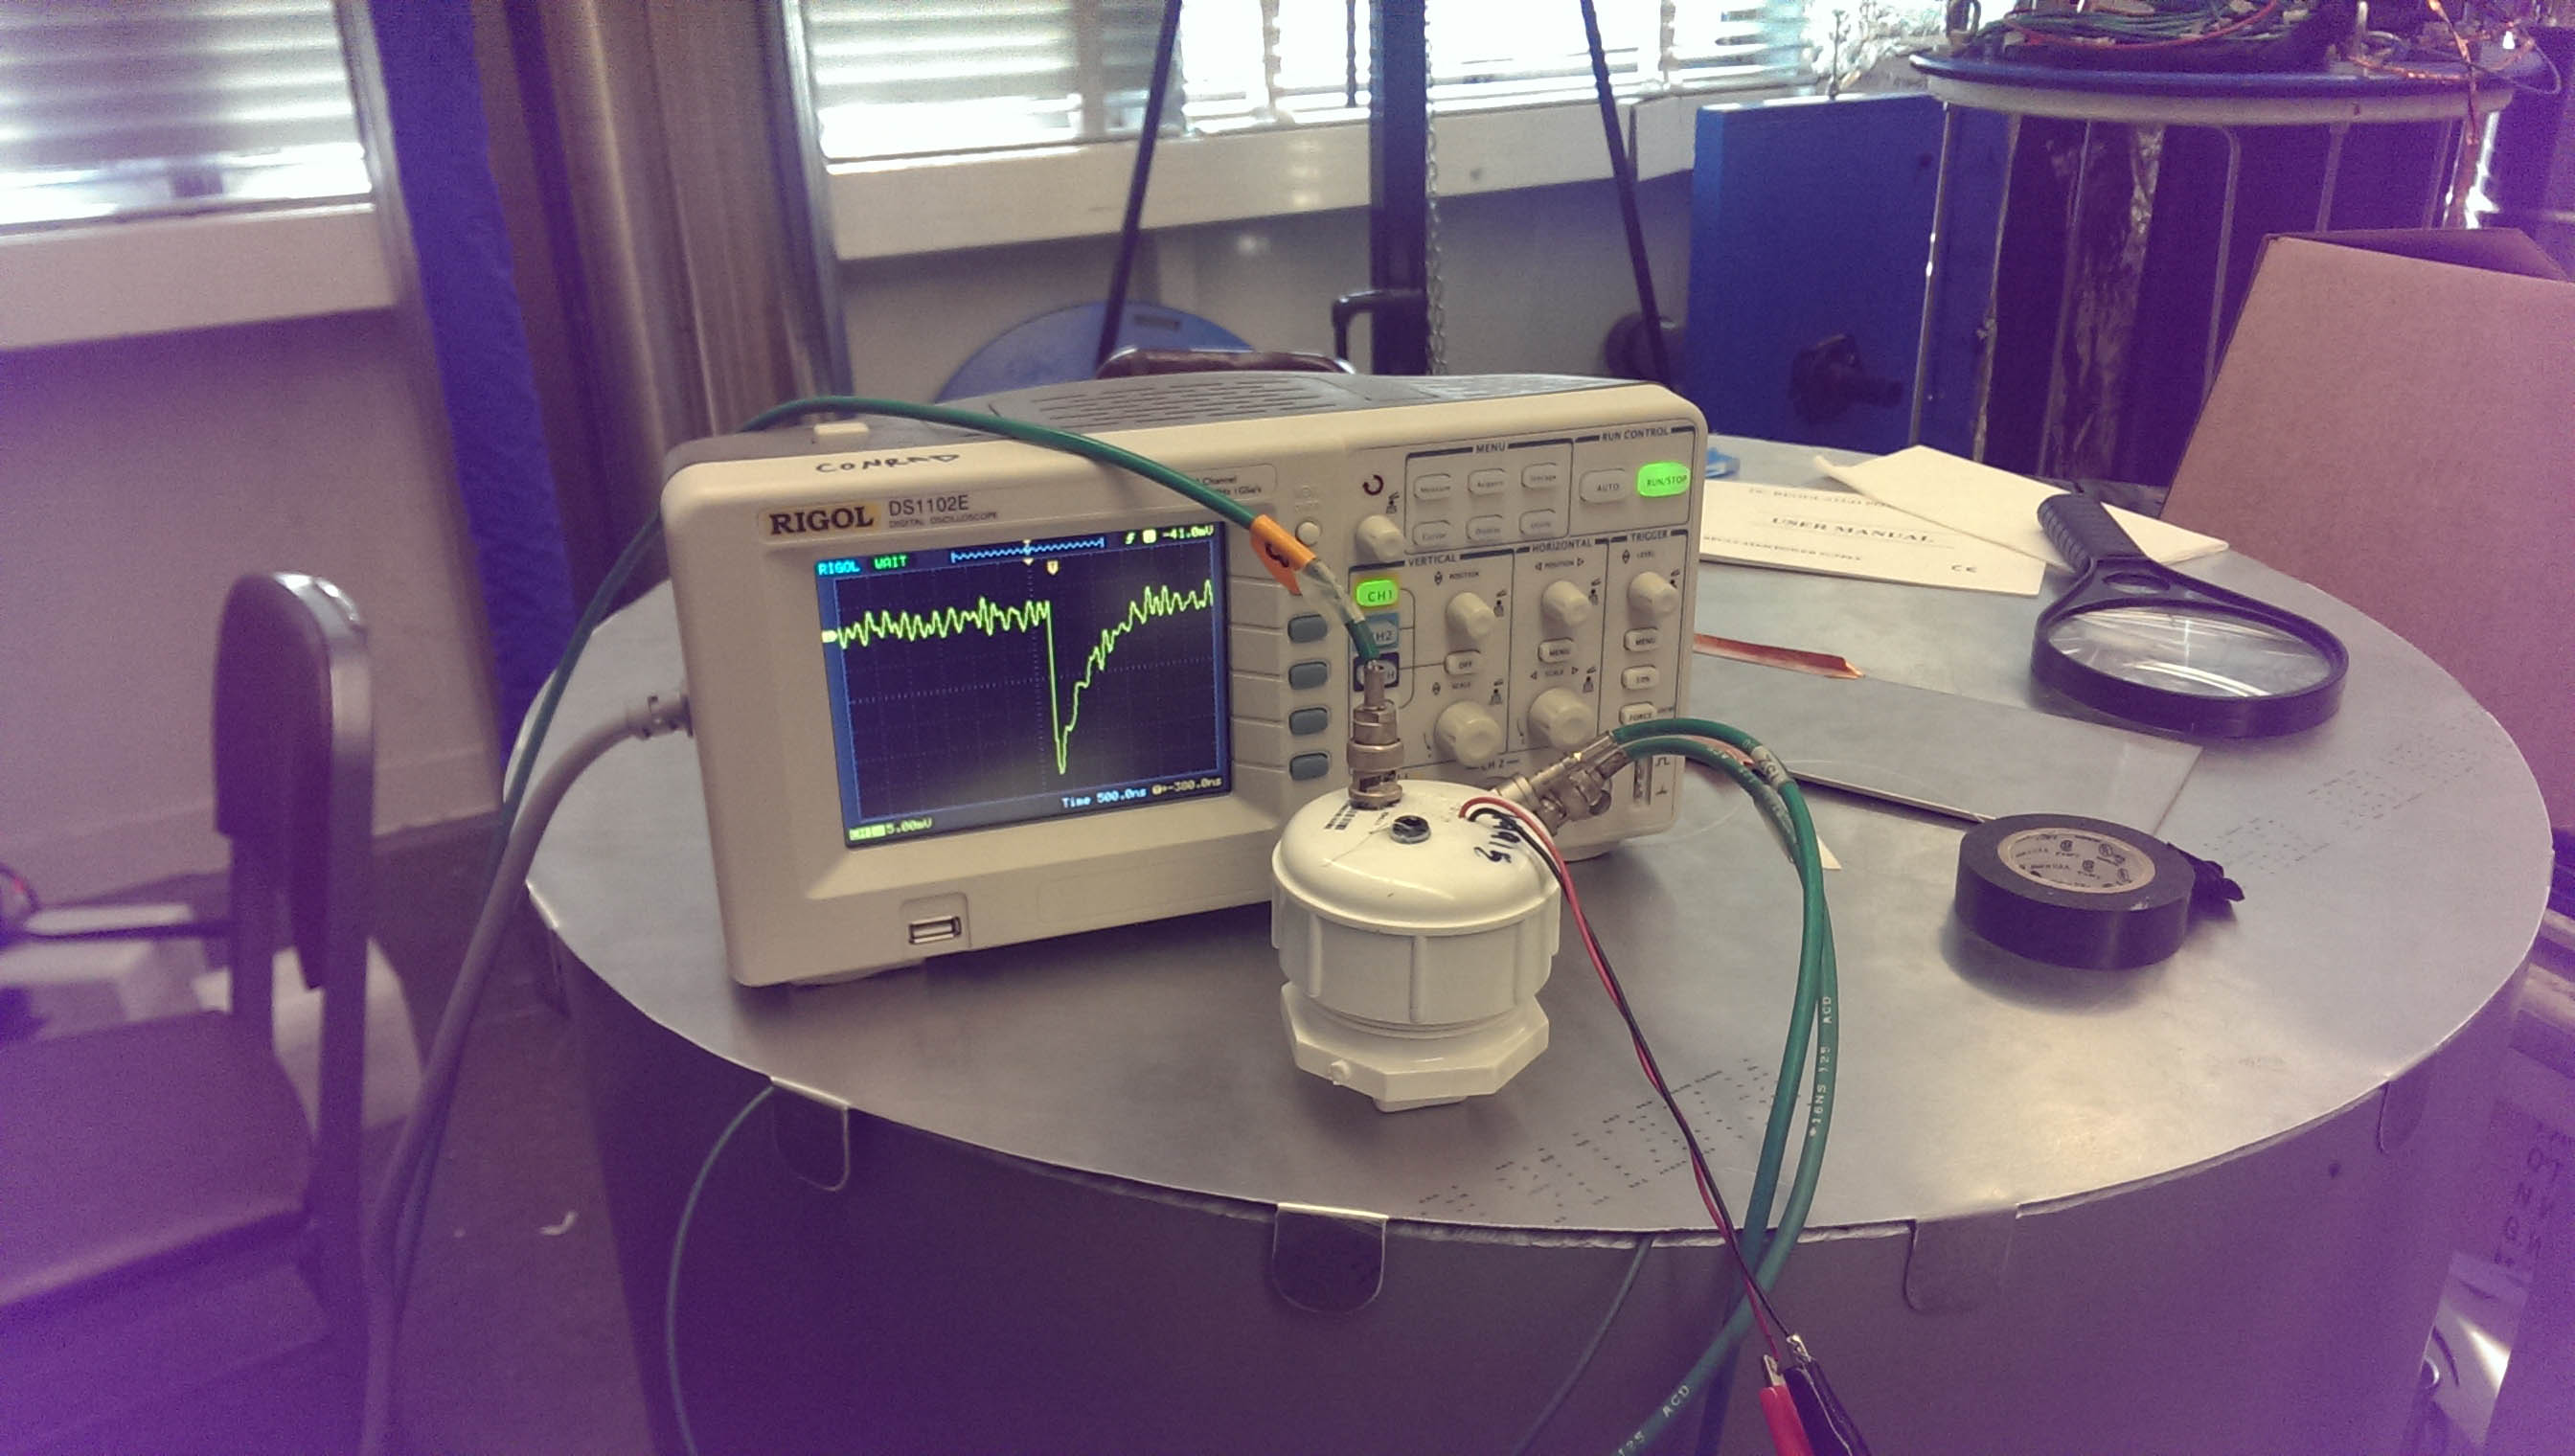
\includegraphics[width=\textwidth]{Detector_description/CW-ver1.jpg}
    \caption{\label{sfig:CW_ver1} First prototype}
  \end{subfigure}
  \begin{subfigure}[t]{0.45\textwidth}
    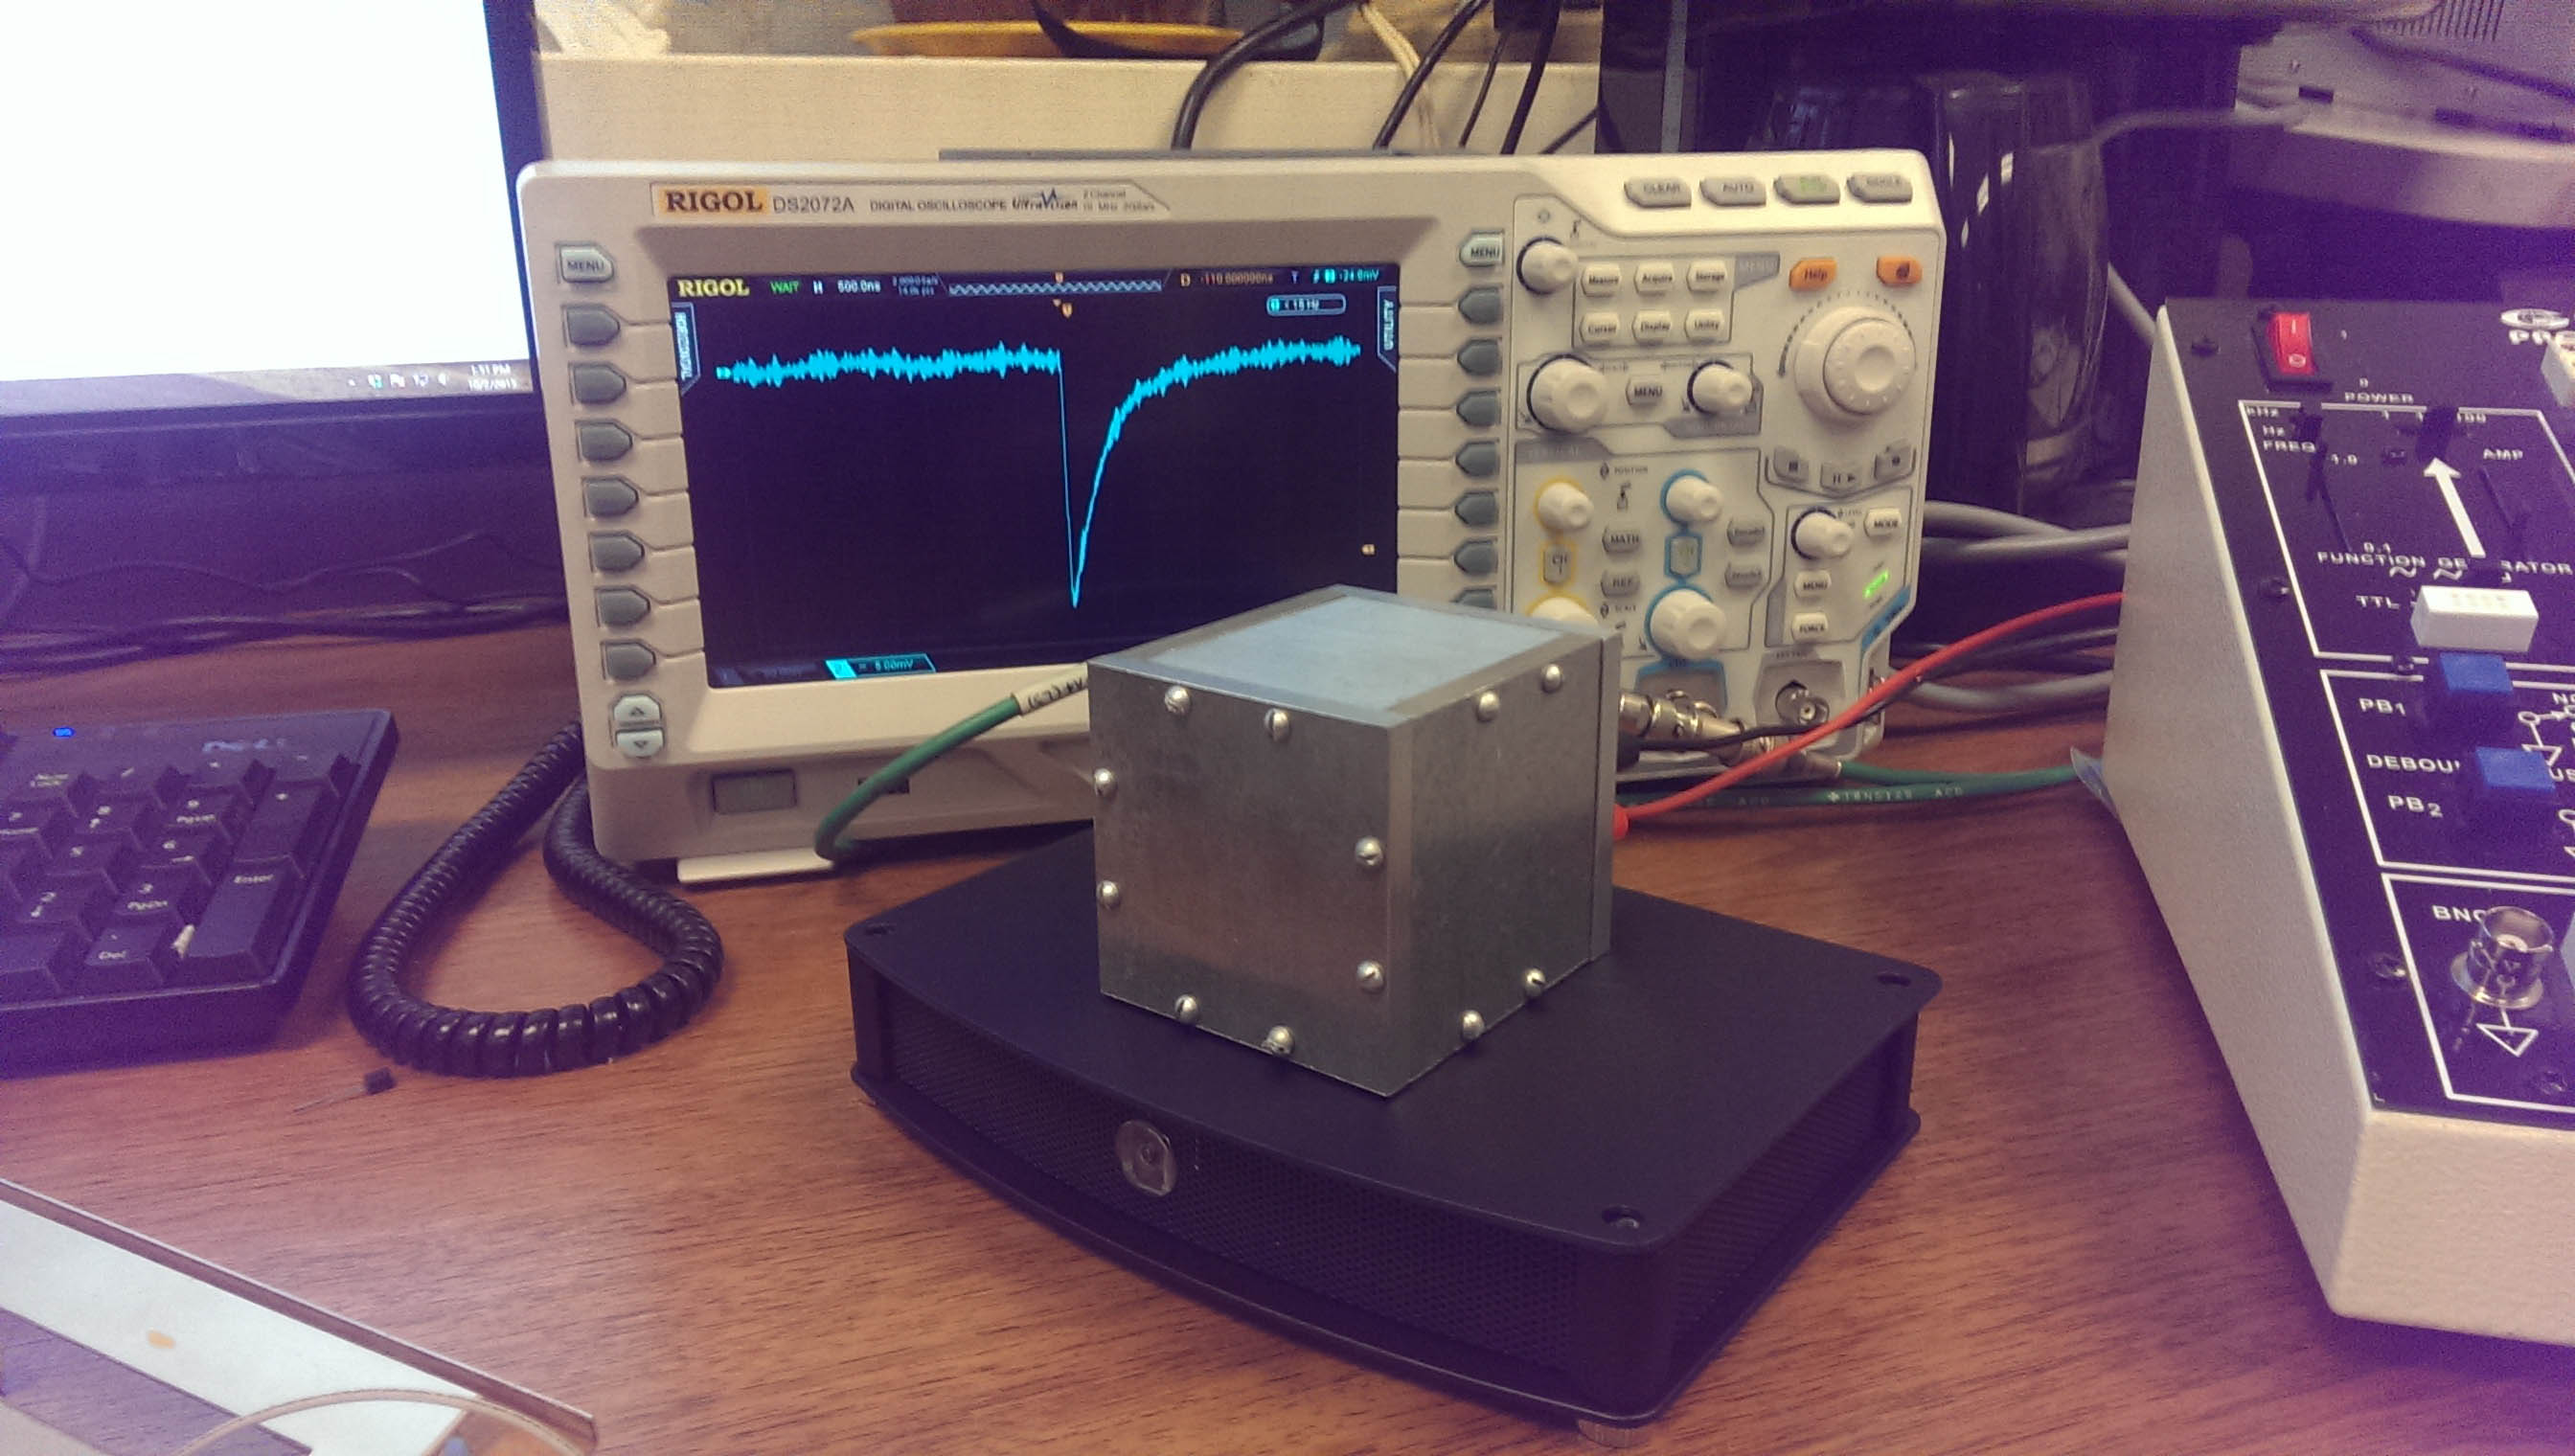
\includegraphics[width=\textwidth]{Detector_description/CW-ver2.jpg}
    \caption{\label{sfig:CW_ver2} Second prototype}
  \end{subfigure}
  \caption{\label{fig:CW_ver1_ver2}First versions of CosmicWatch, prototypes for PINGU, taken from \cite{CosmicWatch}.}
\end{figure}

Later iterations resemble the current goals of CosmicWatch, they are cheaper, smaller, and easier to build. Versions 1 and 2 (Fig. \ref{sfig:CW_ver3}) introduced some user-friendly features, including battery/USB power with $~0.3$ \unit{\watt} consumption, a software-adjustable trigger threshold, and cost about \$100. V2 in particular introduced the use of SD cards to save data and the capability to connect two CosmicWatches, making it possible to measure coincident events.

\begin{figure}[H]
  \centering
  \begin{subfigure}[t]{0.45\textwidth}
    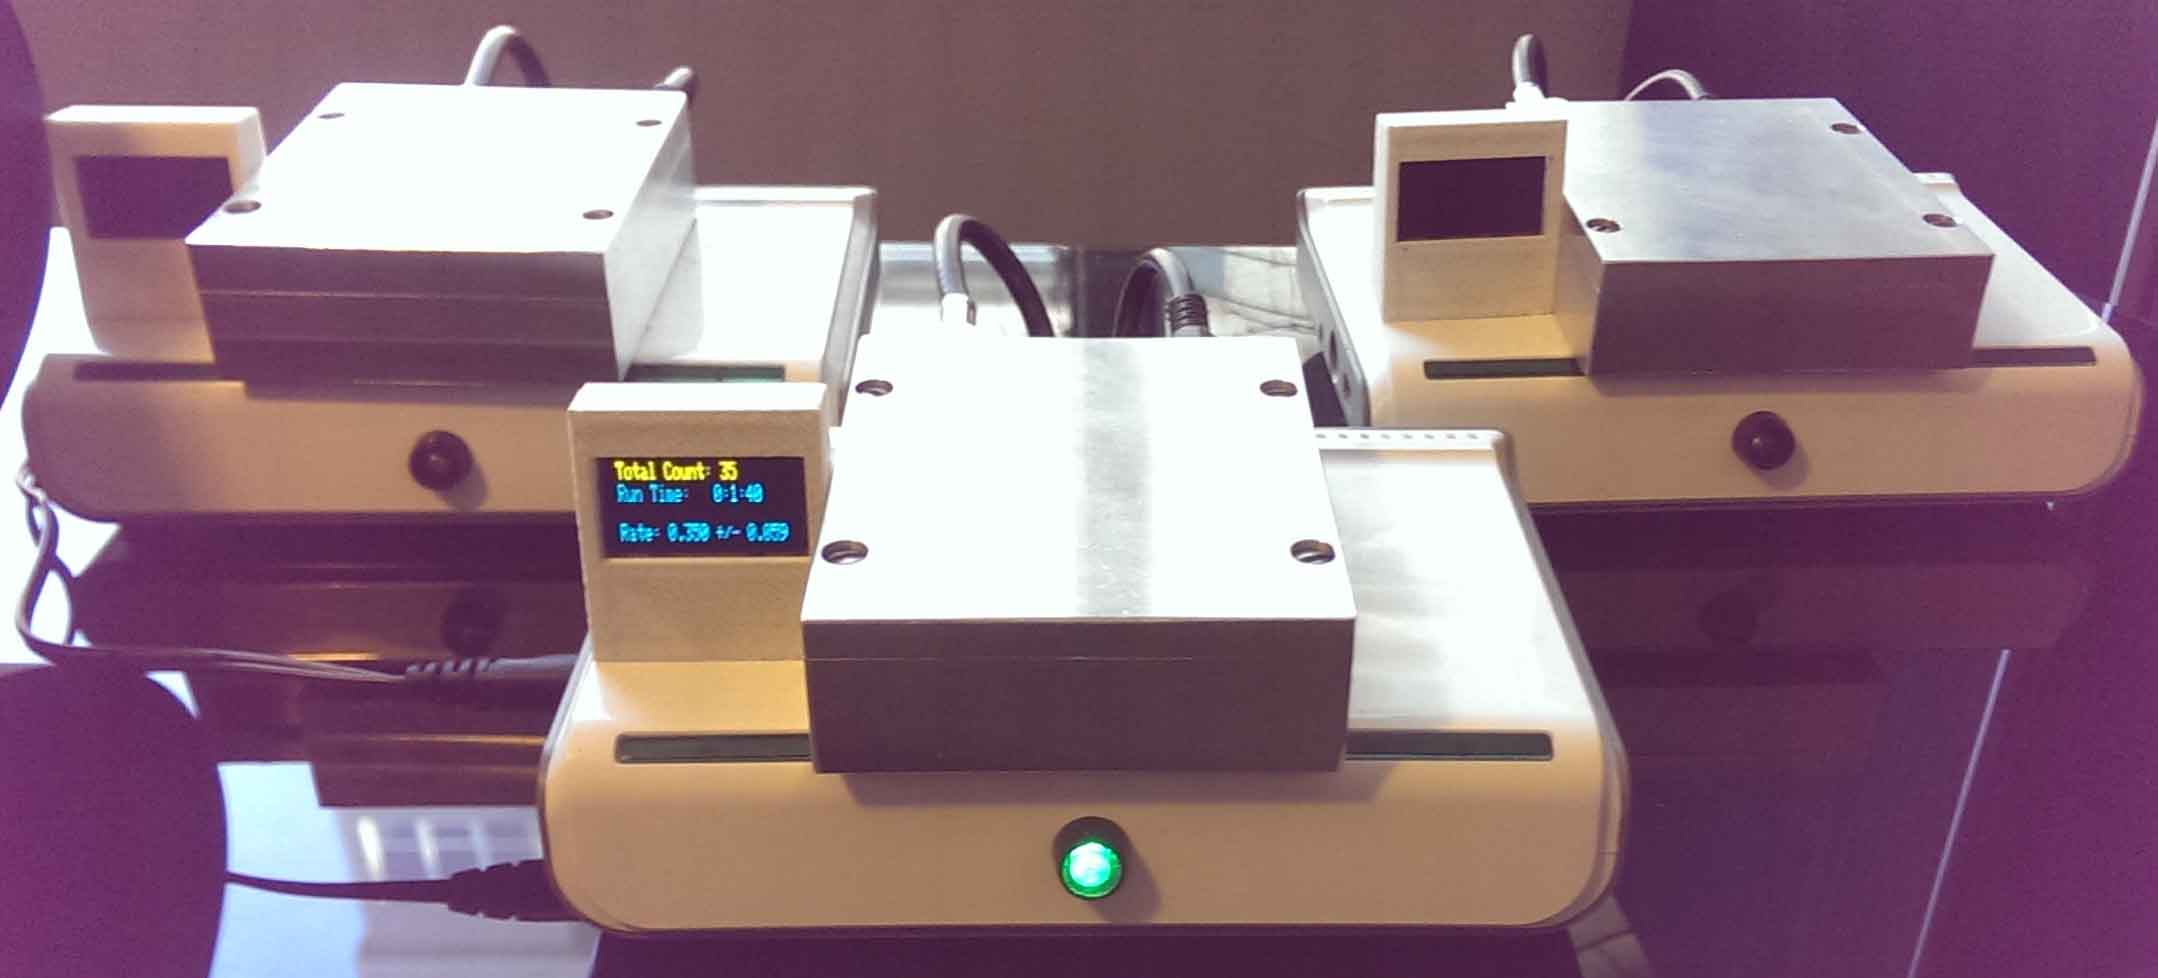
\includegraphics[width=\textwidth]{Detector_description/CW-ver3.jpg}
    \caption{\label{sfig:CW_ver3} Third prototype}
  \end{subfigure}
  \begin{subfigure}[t]{0.45\textwidth}
    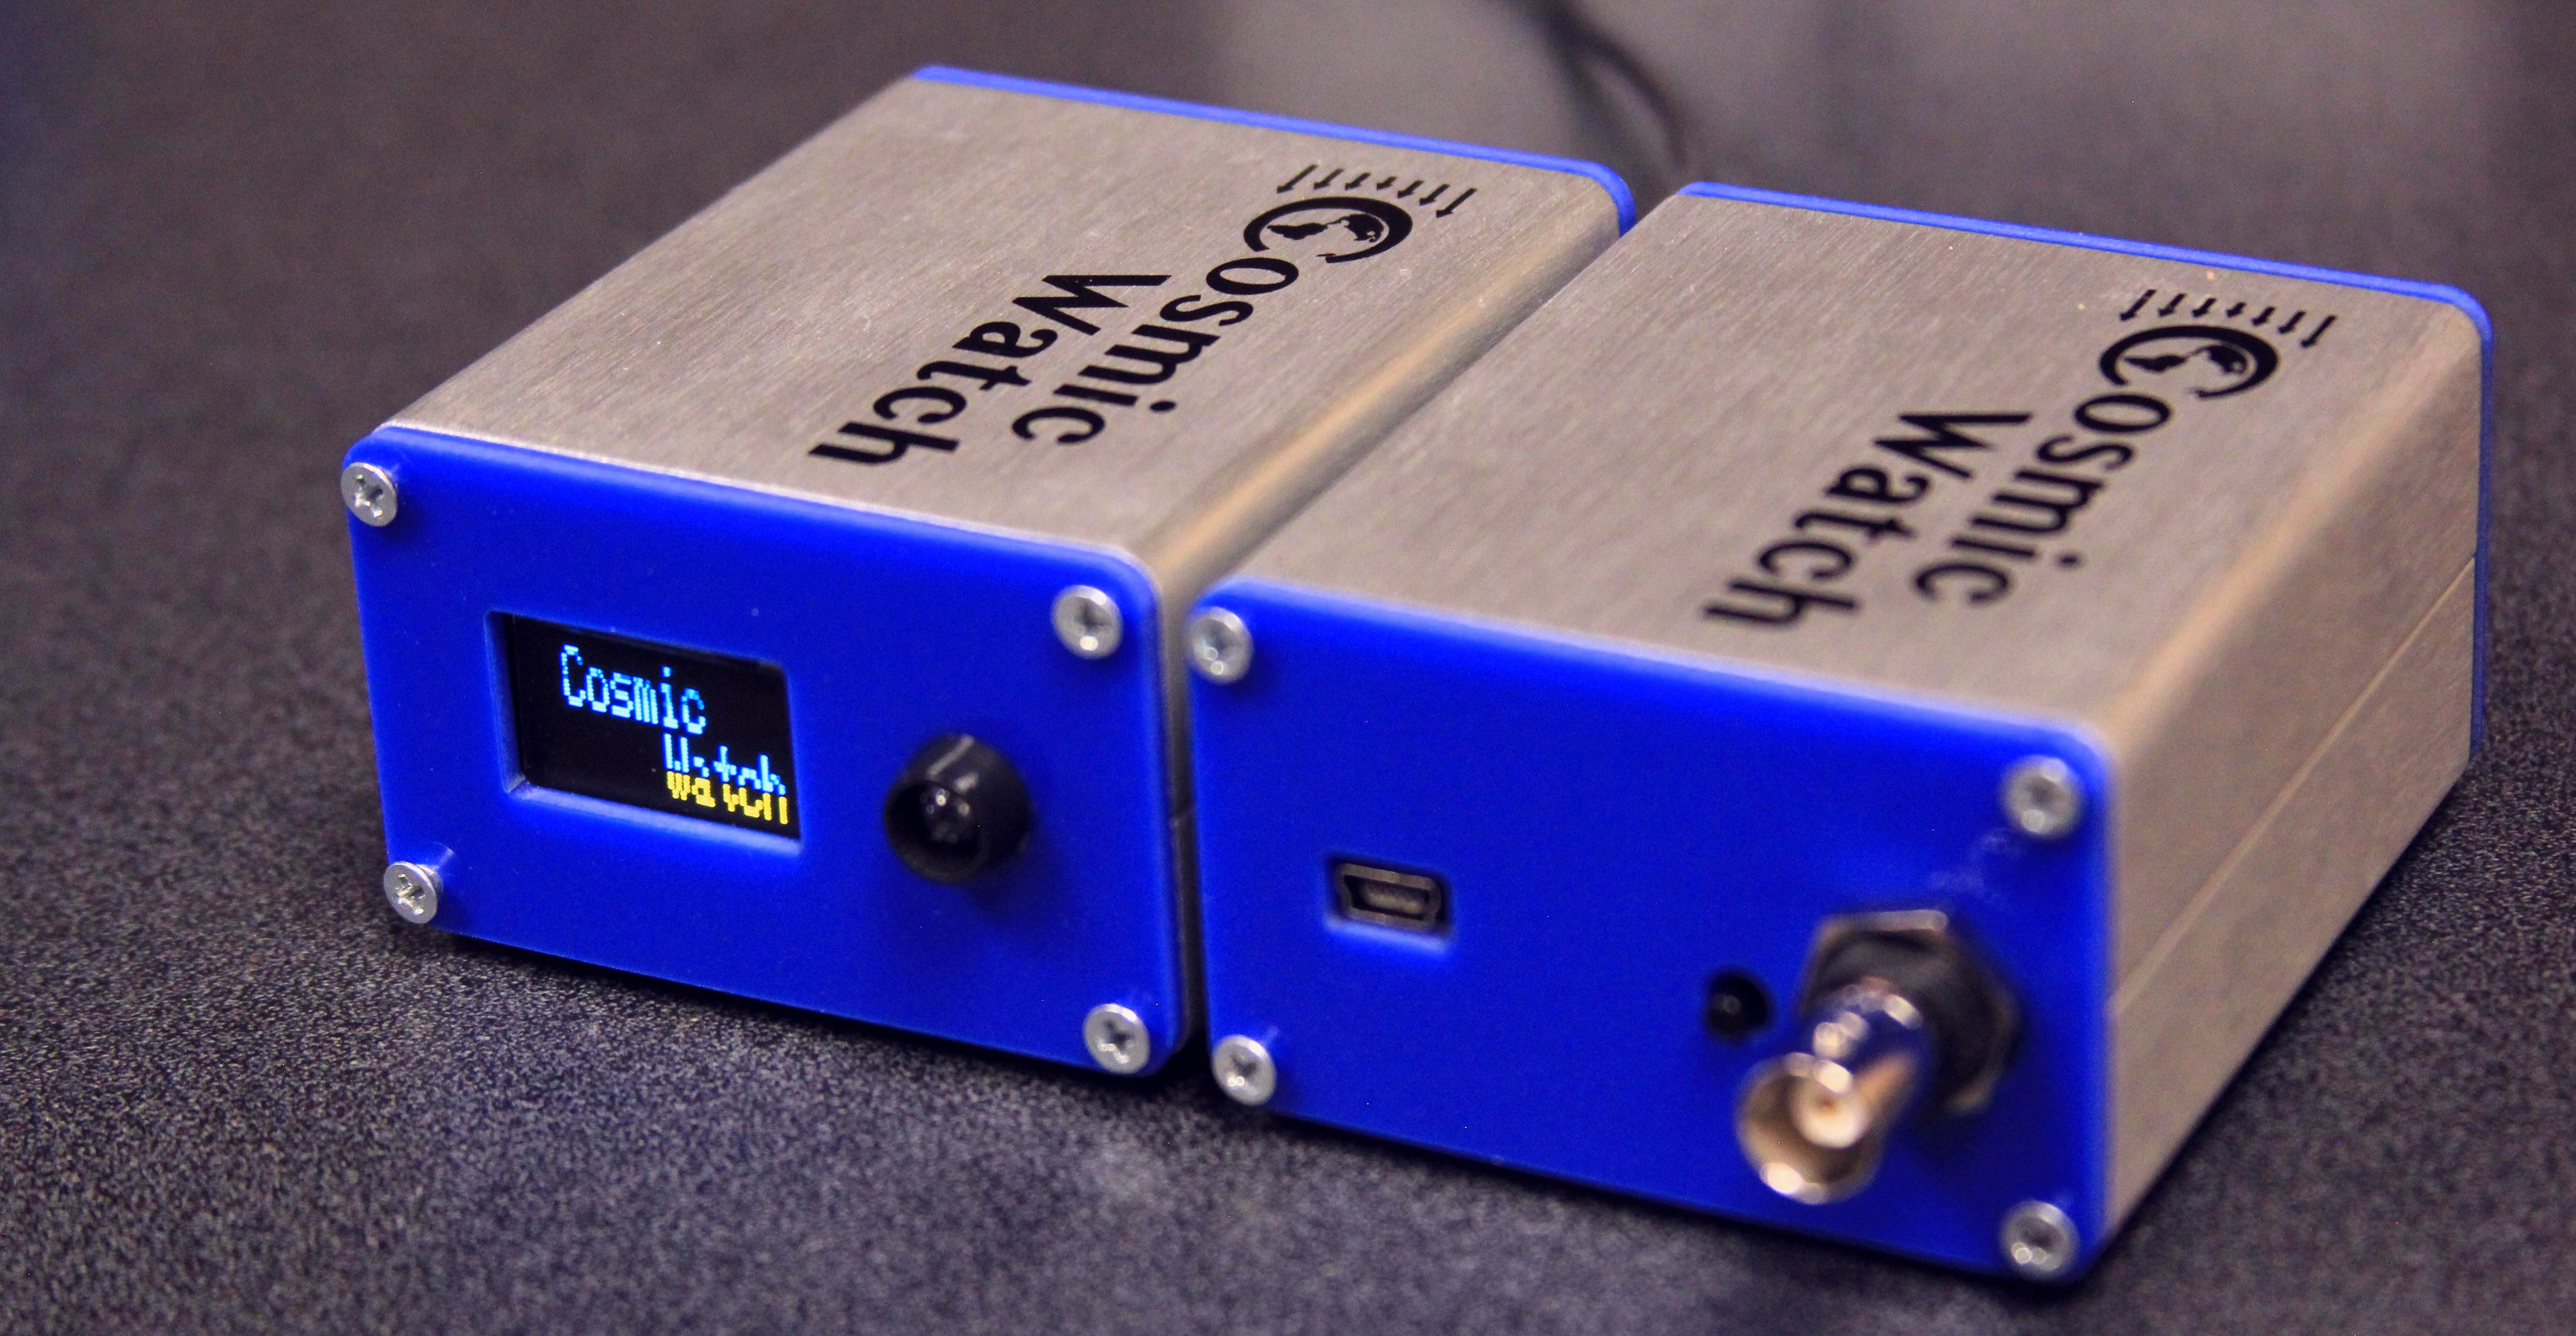
\includegraphics[width=\textwidth]{Detector_description/CW_ver4.jpeg}
    \caption{\label{sfig:CW_ver4} CosmicWatch versions 1 and 2}
  \end{subfigure}
  \caption{\label{fig:CW_ver3_ver4}Newer versions of CosmicWatch, designs suitable for students, taken from \cite{CosmicWatch}.}
\end{figure}

The previous versions of CosmicWatch used an Arduino Nano to process the signal coming from the photomultiplier\footnote{See chapter \ref{chap:Electronics} for an in-depth description of the inner workings of the detector electronics}, which has only one core. This is a disadvantage when there is a high event rate since one can not sample data while saving previous events. The use of a Raspberry Pi Pico is one of the main improvements in upcoming versions of CosmicWatch, its two cores allow to sample data in one thread while the other handles serial communication to save previous events. This will reduce deadtime, making it suitable for high event rates, such as those found around active gamma sources.

\section{Plastic vs. LYSO}

Up until now, due to how affordable and malleable they can be, only plastic scintillators have been used, particularly Polyvinyltoluene-based scintillators such as BC-400 and BC404. Sadly, it is well known that their poor energy resolution and lack of linearity makes them useless for gamma spectroscopy, at least in small sizes as the ones used for CosmicWatch ($5\times5\times1$ \unit{\cm\cubed}). In addition to this, plastic scintillators have very low light yields $10000$ photons/MeV \cite{mukhopadhyay2004plastic}, making it hard to detect low-energy events. Table \ref{tab:scintillators} compares the general properties of some scintillating materials, better showcasing the advantages of LYSO in particular for gamma spectroscopy in the CosmicWatch context.

\begin{table}[htb]
  \caption{General properties of some scintillating materials. Taken from \cite{mukhopadhyay2004plastic,Luxium_LYSO,Luxium_plastic,SaintGobain_NaI}. $^*$Calculated from the attenuation coefficient at 662 \unit{\kilo\eV} shown in \cite[p.~3]{SaintGobain_NaI}}
  \centering
  \begin{tabular}{ l c c c c}
    \midrule
    Property & LYSO & BC-400 & NaI(TI) & BGO\\
    \midrule
    Density [\unit{\g\per\cm\cubed}] & 7.1 & 1.032 & 3.67 & 7.1\\
    Decay time [\unit{\nano\s}]  & 36 & 2.4 & 250 & 300\\
    Light yield [\unit{ph\per\mega\eV}] & 33200 & 10000 & 38000 & 9000\\
    Attenuation Length at 511 \unit{\kilo\eV} [\unit{\cm}] & 1.2 &  & $3.3^{*}$ & 1.0\\
    \bottomrule
  \end{tabular}
  \label{tab:scintillators}
\end{table}

Higher densities are good for energy deposition, catching particles and gammas more efficiently. Short decay times allow to make fast signal pulses. High light yields make it possible to detect low-energy events. Short attenuation lengths decrease the amount of material necessary to get energy depositions.

\section{Power Consumption}

\section{KiCad}

KiCad is an opensource software that allows to create circuit schematics, PCB layout, and 3D viewing among other capabilities. It is available in Windows, Linux and iOS, making it perfect for CosmicWatch, since on of the goals is to make it easily available to new users. The KiCad project for CosmicWatch V2 can be found on the repository \href{https://github.com/spenceraxani/CosmicWatch-Desktop-Muon-Detector-v2}{CosmicWatch-Desktop-Muon-Detector-v2} under ``PCB\_Files''.

\href{https://github.com/anvargasl/CosmicWatch-gamma-spectroscopy-PCB}{CosmicWatch-gamma-spectroscopy-PCB} contains the KiCad files necessary to build the newer version of CosmicWatch, all the necessary footprints can be found in ``MyLibrary.pretty'', including the Raspberry Pi Pico footprints. In order to print the PCB it is necessaty to send the compressed ``Geber'' folder (found under ``CosmicWatch\_detector\_v33'') to a manufacturer, \href{https://www.elecrow.com/pcb-manufacturing.html}{ELECROW} is recommended.

\section{Accessories}

Currently CosmicWatch includes some accessories that make it possible to customize the detector and get more specific measurements, making use of its multiple sensors and features. Drivers and example code necessary to control the accessories listed bellow are included in \href{https://github.com/anvargasl/CosmicWatch-gamma-spectroscopy-RP}{CosmicWatch-gamma-spectroscopy-RP} under the ``drivers'' folder.

\subsection{Preassure and Temperature sensor}

\begin{figure}[H]
  \centering
  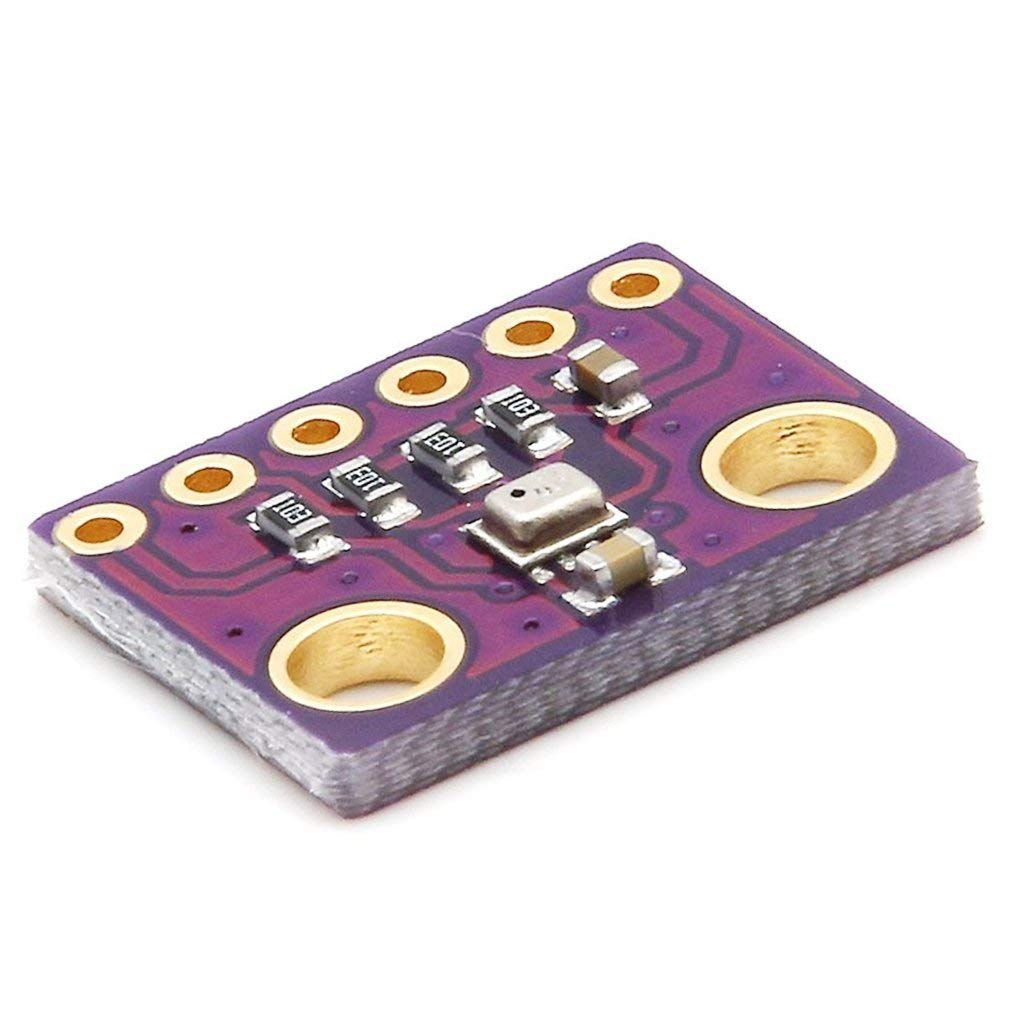
\includegraphics[width=0.4\textwidth]{Detector_description/bmp280.jpg}
  \caption{BMP280 sensor PCB example, it can be easily found online. Taken from \href{https://a.co/d/hhF7Vtp}{Amazon}.}
  \label{fig:bmp280}
\end{figure}

An absolute barometric pressure sensor \href{https://www.bosch-sensortec.com/products/environmental-sensors/pressure-sensors/bmp280/}{BMP280} can be included in the detector construction to make barometric measurements that can relate to muon counts. Temperature can also affect the SiPM and LYSO response, possibly making this data important while characterizing the detector. The Raspberry Pi Pico has a built in temperature sensor, this however has been found to have some errors dependig on the reference voltage, making its calibration necessary.

The Raspberry Pi Pico reads data from the BMP280 through the I2C protocol, the MicroPython driver can also be found in \href{https://github.com/dafvid/micropython-bmp280}{micropython-bmp280} by David Stenwall, who has made an amaizing description on the use of this sensor in his repository.

\subsection{OLED screen}

\begin{figure}[H]
  \centering
  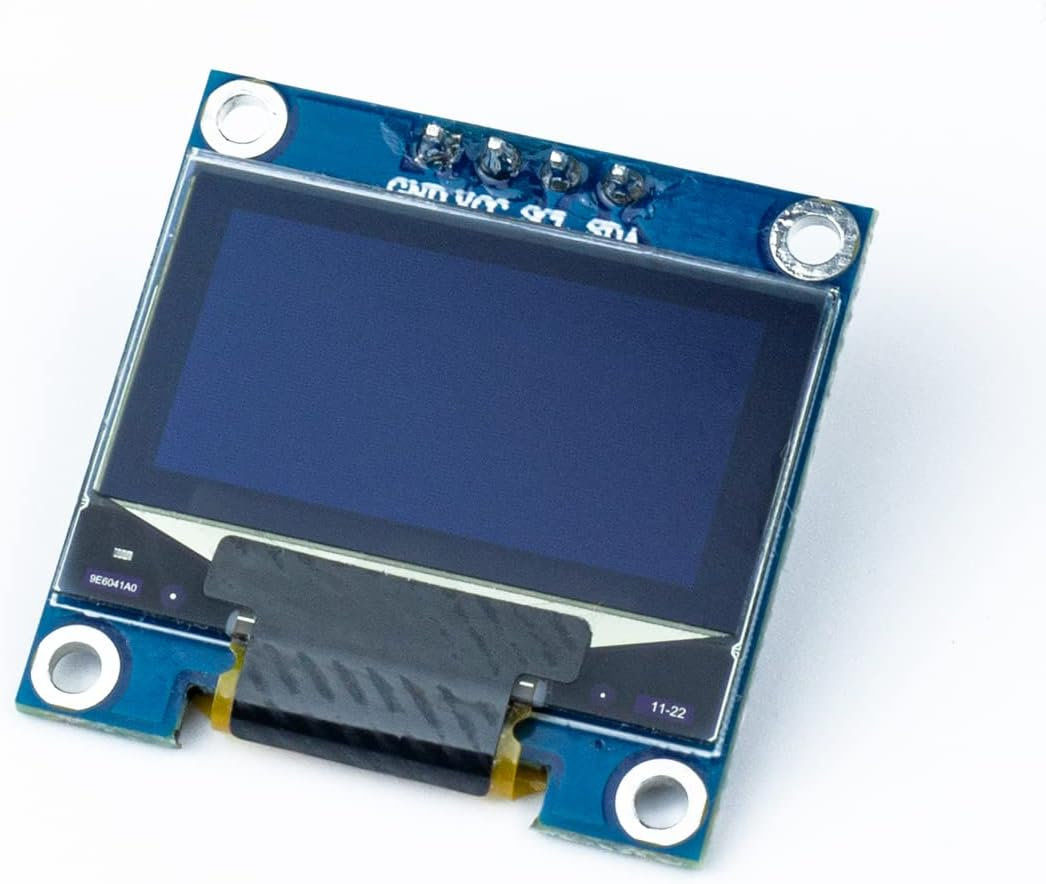
\includegraphics[width=0.4\textwidth]{Detector_description/ssd1306.jpg}
  \caption{SSD1306 OLED screen example, it can be easily found online. Taken from \href{https://a.co/d/cGnBDLF}{Amazon}}
  \label{fig:bssd1306}
\end{figure}

OLED screens are versitalie and provide a fast way to read data directly from the detector, making it more user friendly and easier to trouble-shoot. An ssd1306 OLED screen can be connected to the detector, the driver is listed in the \href{https://github.com/micropython/micropython-lib/tree/master/micropython/drivers/display}{MicroPython documentation}.

The ``Login'' screen of the detector shows a $128\times 64$ pixelart on bytearray form of the CosmicWatch logo, found under the ``Logos'' in \href{https://github.com/anvargasl/CosmicWatch-gamma-spectroscopy-RP}{CosmicWatch-gamma-spectroscopy-RP}.

\section{3D printed case}

In order to hold the crystal in place on the SiPM PCB, it was necessary to design a 3D printed case -see Fig. \ref{fig:3d_case_desing} for an image of the 3D design on Inventor. With this we made sure that the crystal would not move relative to the SiPM, preventing scratches and providing a more stable optical coupling with the photomultiplier.

\begin{figure}[H]
    \centering
    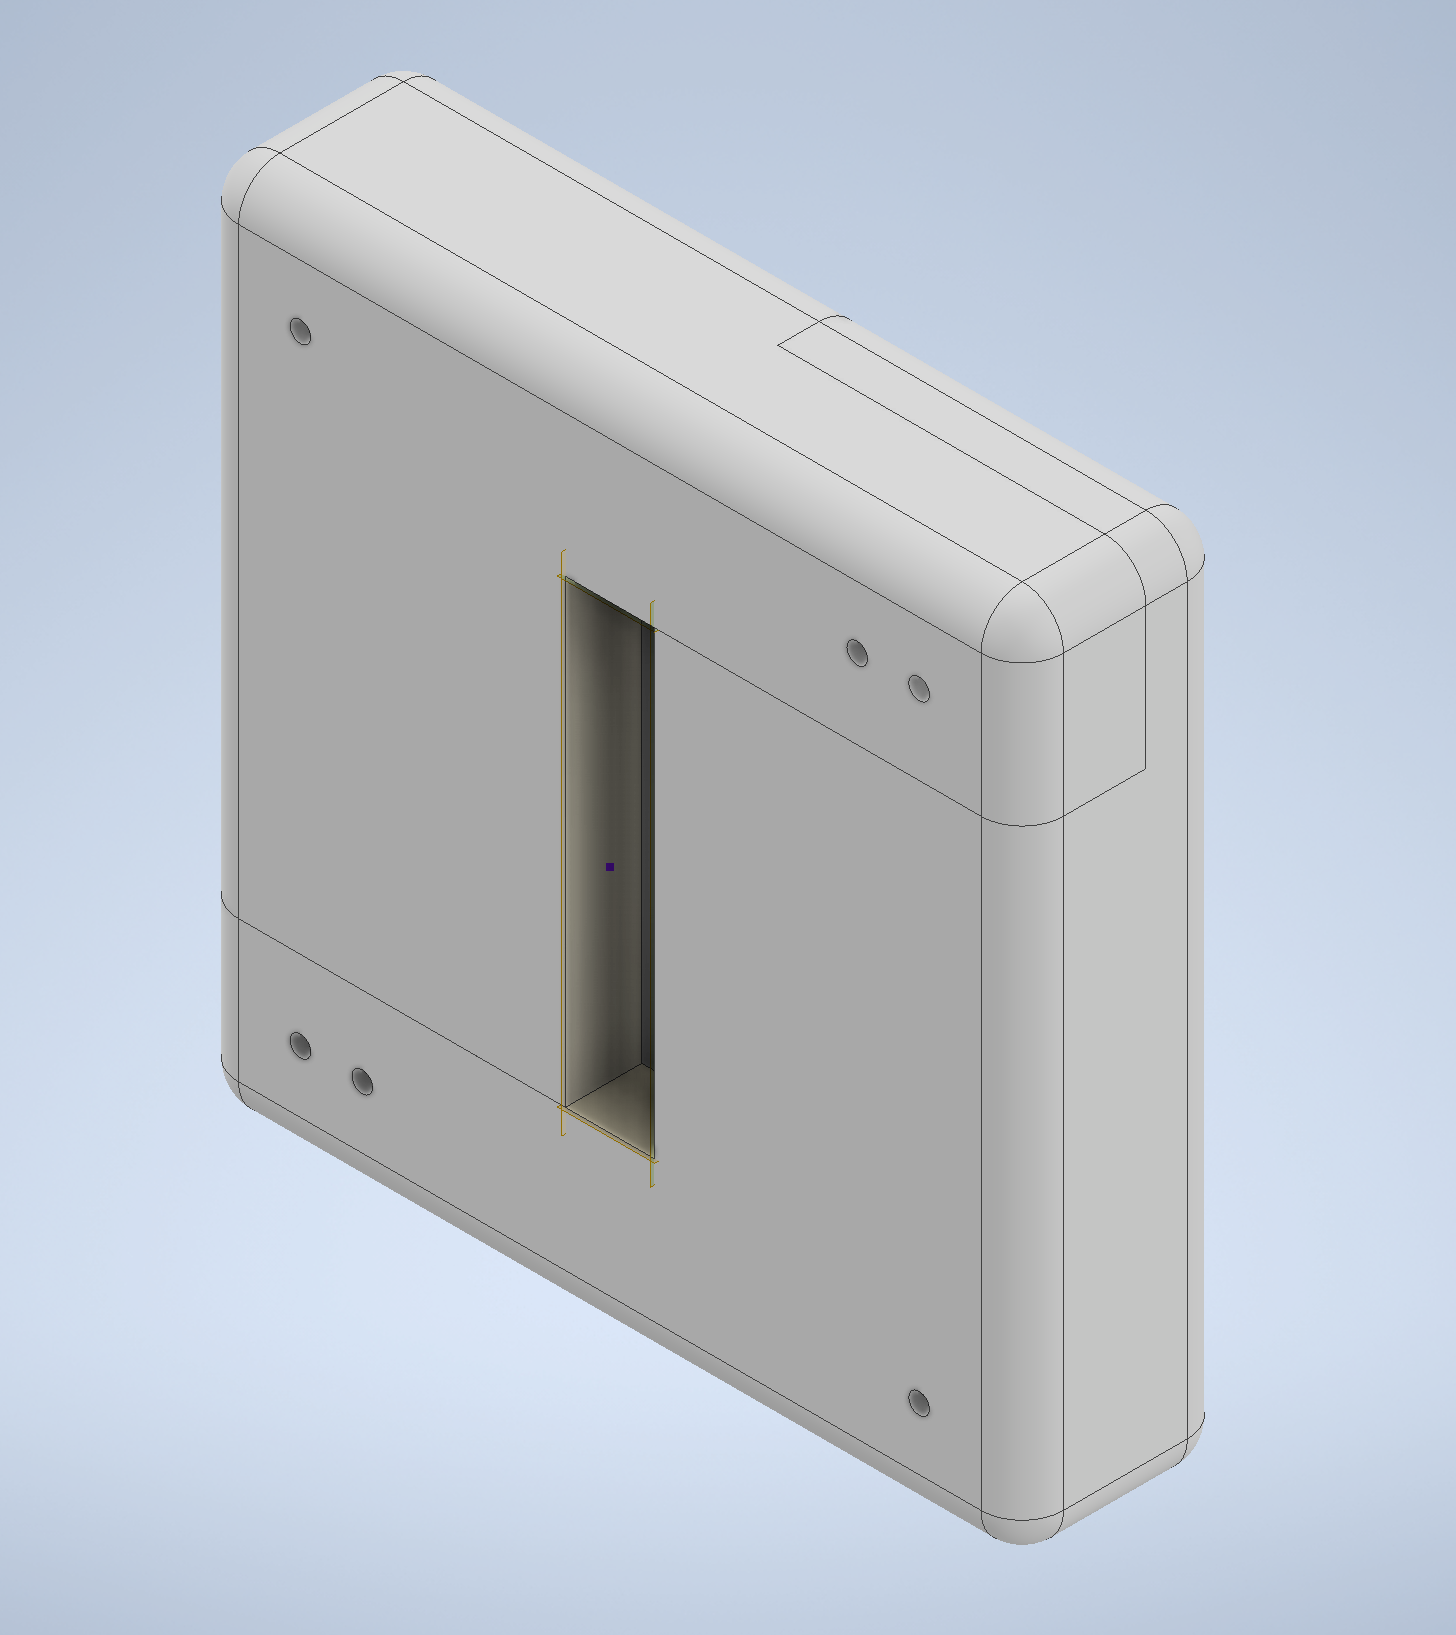
\includegraphics[width=0.6\textwidth]{Detector_description/3d_case_inventor.png}
    \caption{3D model of the LYSO case made on Inventor, the .cad files can be found on the repository \href{https://github.com/anvargasl/CosmicWatch-gamma-spectroscopy-PCB}{CosmicWatch-gamma-spectroscopy-PCB}.}
    \label{fig:3d_case_desing}
\end{figure}

The design keeps in mind that the crystal has to be wrapped in Teflon tape to increase reflectivity, which is why it comes in two pieces that come together around the crystal, lowering the risk of tears. Once the crystal is placed in the case it can be kept together using electrical tape.

Before using Teflon tape, the crystal was wrapped in tin foil, which made tears common (Fig. \ref{fig:tin_foil_tear}) and greatly impacted the quality of the spectra that could be obtained with the detector. 

\begin{figure}[H]
    \centering
    \begin{subfigure}[t]{0.45\textwidth}
      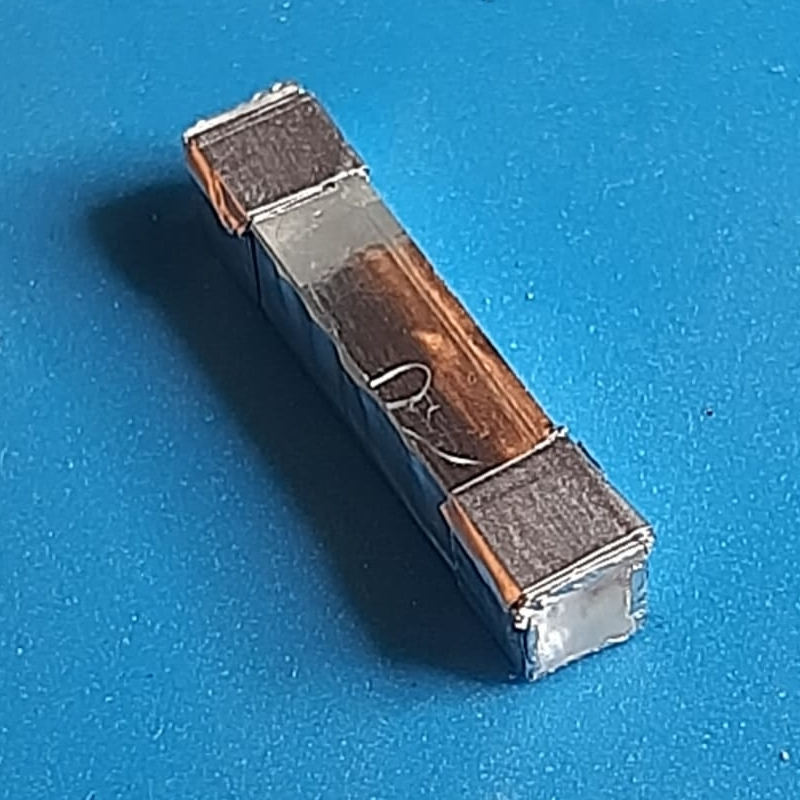
\includegraphics[width=\textwidth]{Detector_description/LYSO-wrapped.jpeg}
    \end{subfigure}
    \begin{subfigure}[t]{0.45\textwidth}
      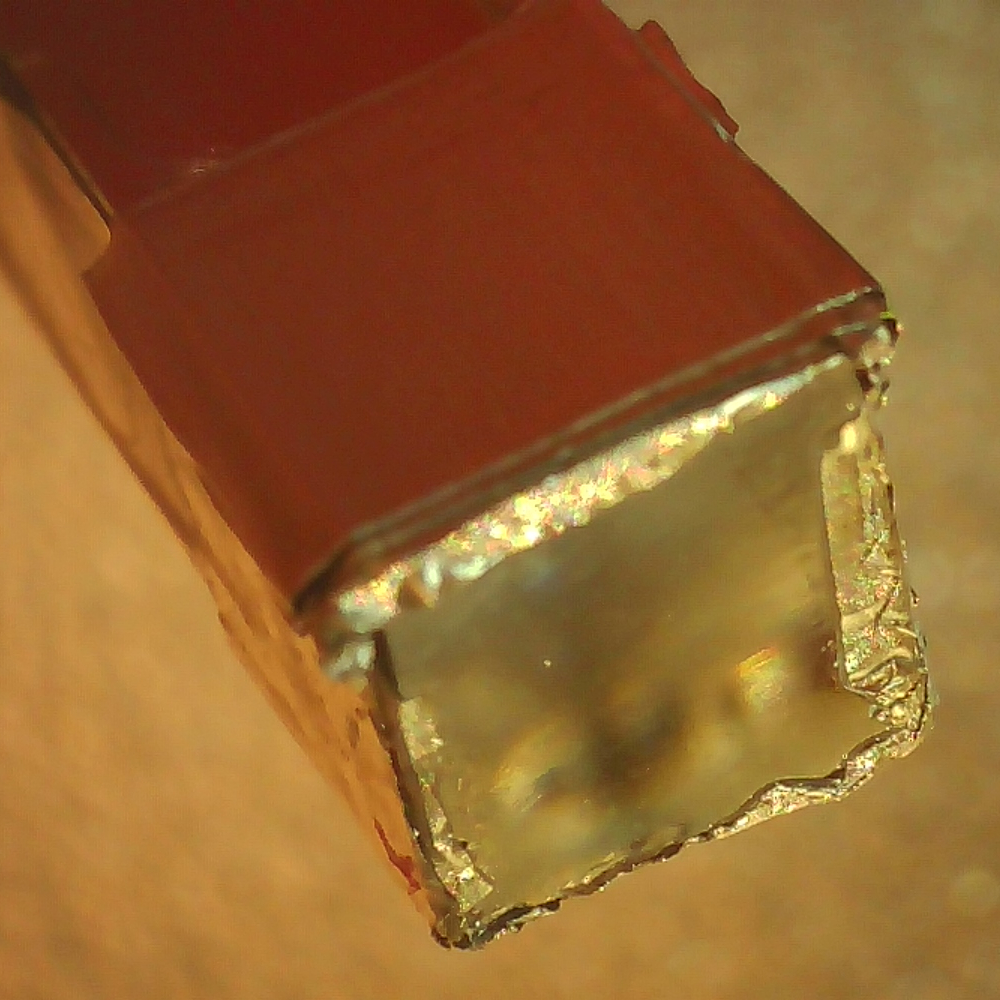
\includegraphics[width=\textwidth]{Detector_description/tin_foil_tear.jpg}
    \end{subfigure}
    \caption{\label{fig:tin_foil_tear}Tin foil tear.}
\end{figure}

Teflon tape seems to solve the tearing problem. However, to reduce the risk of tearing the Teflon, multiple iterations of the case were designed (Fig. \ref{fig:3d_previous_desings})

\begin{figure}[H]
    \centering
    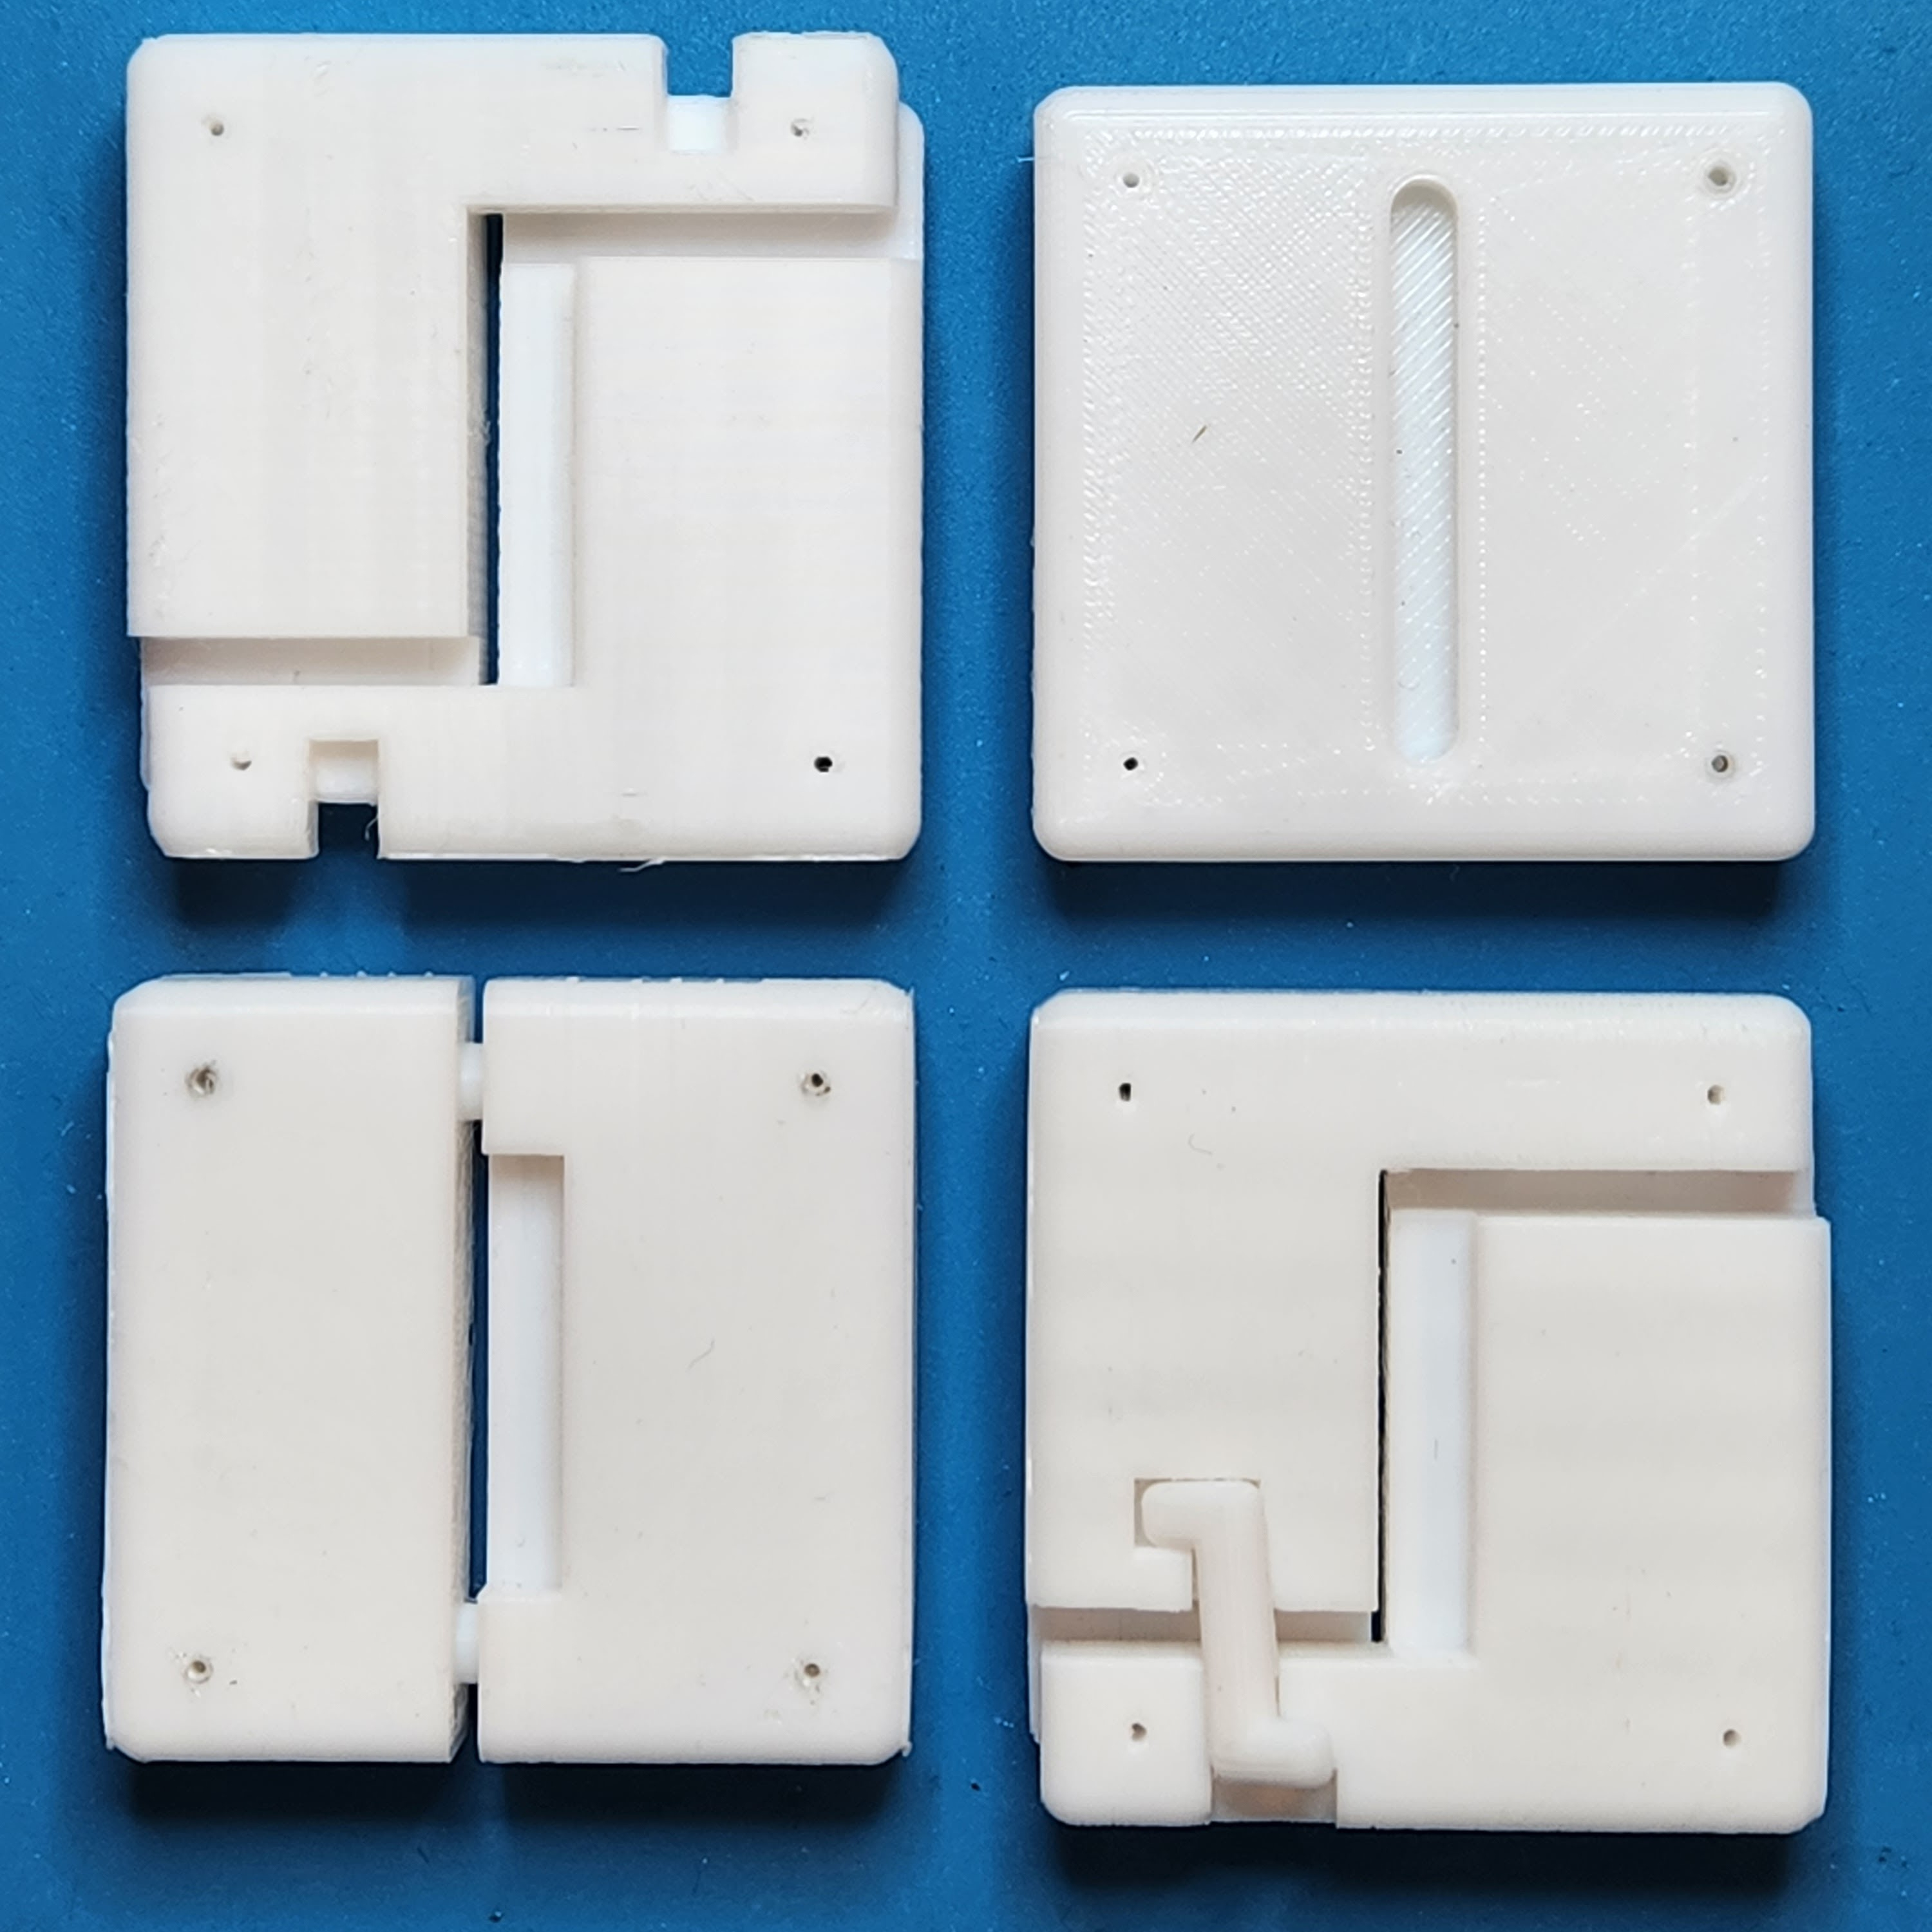
\includegraphics[width=0.6\textwidth]{Detector_description/Holder-designs.jpeg}
    \caption{3D printed cases tested to reduce the risk of Teflon tears.}
    \label{fig:3d_previous_desings}
\end{figure}

\chapter{Detection methods} \label{chap:detection_methods}

%versions of the detector
\section{Scintillation}

\section{Single photon detectors}

\section{PMTs}

Photomultipliers are very useful tools in particle detection. Since some detection methods rely on the measurement of photons it is very important to make use of every single one. Some PMs are capable of creating measurable electrical signals from single photon interactions, provoking an electron avalanche that can be easily read with various devices. Photomultiplier Tubes are the most common light amplifiers paired with scintillators, they are however bulky and require very high voltages to operate. An in-depth description of this and other types of Photomultipliers can be found in Ref. \cite{knoll2010radiation} Chap. 9.

\section{SiPM advantages}

CosmicWatch is meant to be a portable, easy-to-build, and economical device, making PMTs not suitable for the overall intention of the project. This, however, is fully solved by Silicon Photomultipliers, their small form factor, relatively low operating voltage, and good efficiency at wavelengths near the emission maxima of common scintillating materials, turn them into an ideal candidate for use in this project. For further details on SiPMs also read Ref. \cite{knoll2010radiation} Chap. 9 and Ref. \cite{Onsemi_SiPM_intro}.

A Silicon Photomultiplier is an array of Geiger-mode avalanche-photodiodes. To make this more digestible we can introduce these concepts one by one. A photodiode is essentially made of a P-N semiconductor junction, where scintillation photons can create new electron-hole pairs that will be accelerated by the bias voltage applied to the diode. However, this process alone produces small signals, making a preamplification stage necessary. Avalanche photodiodes alleviate this problem by increasing the bias voltage, therefore giving the photoelectrons higher energies, allowing them to collide and produce new electron-hole pairs that will also be detected. When the bias voltage rises sufficiently high, the regions where photoelectrons multiply merge together, making one big avalanche, this is the so-called Geiger mode of APDs, and this high voltage receives the name of Breakdown Voltage. Geiger mode APDs can produce a large output from a single scintillation photon. The difference Between Bias and Breakdown Voltage is known as Over-voltage.

SiPMs however, also have some disadvantages, since they are based on the transport of photoelectrons, the output can vary with temperature, as high temperatures can create electron-hole pairs that will be read as a photon interaction. These events are called dark pulses and represent a random noise in the signal.

The SiPM used and tested throughout this work is a MicroFJ-300XX-TSV by Onsemi \cite{Onsemi_SiPM} (Fig. \ref{fig:Onsemi_SiPM}), which has an active area of $3.07 \times 3.07$ \unit{\mm\squared} and a microcell size of 35 \unit{\micro\m}. In this case, the operating voltage ranges between 25.2 and 30.7 \unit{\V}, which can be obtained using a DC to DC booster (see Section \ref{sec:DC_DC}), no longer requiring the high voltages of PMTs. We are currently operating at an Over-voltage of 4 V, which according to Ref. \cite{Onsemi_SiPM} produces a relatively high dark count rate (50-150 \unit{\kilo\Hz\per\mm\squared} at 21 $^\circ$C), potentially affecting energy resolution.

\begin{figure}[H]
    \centering
    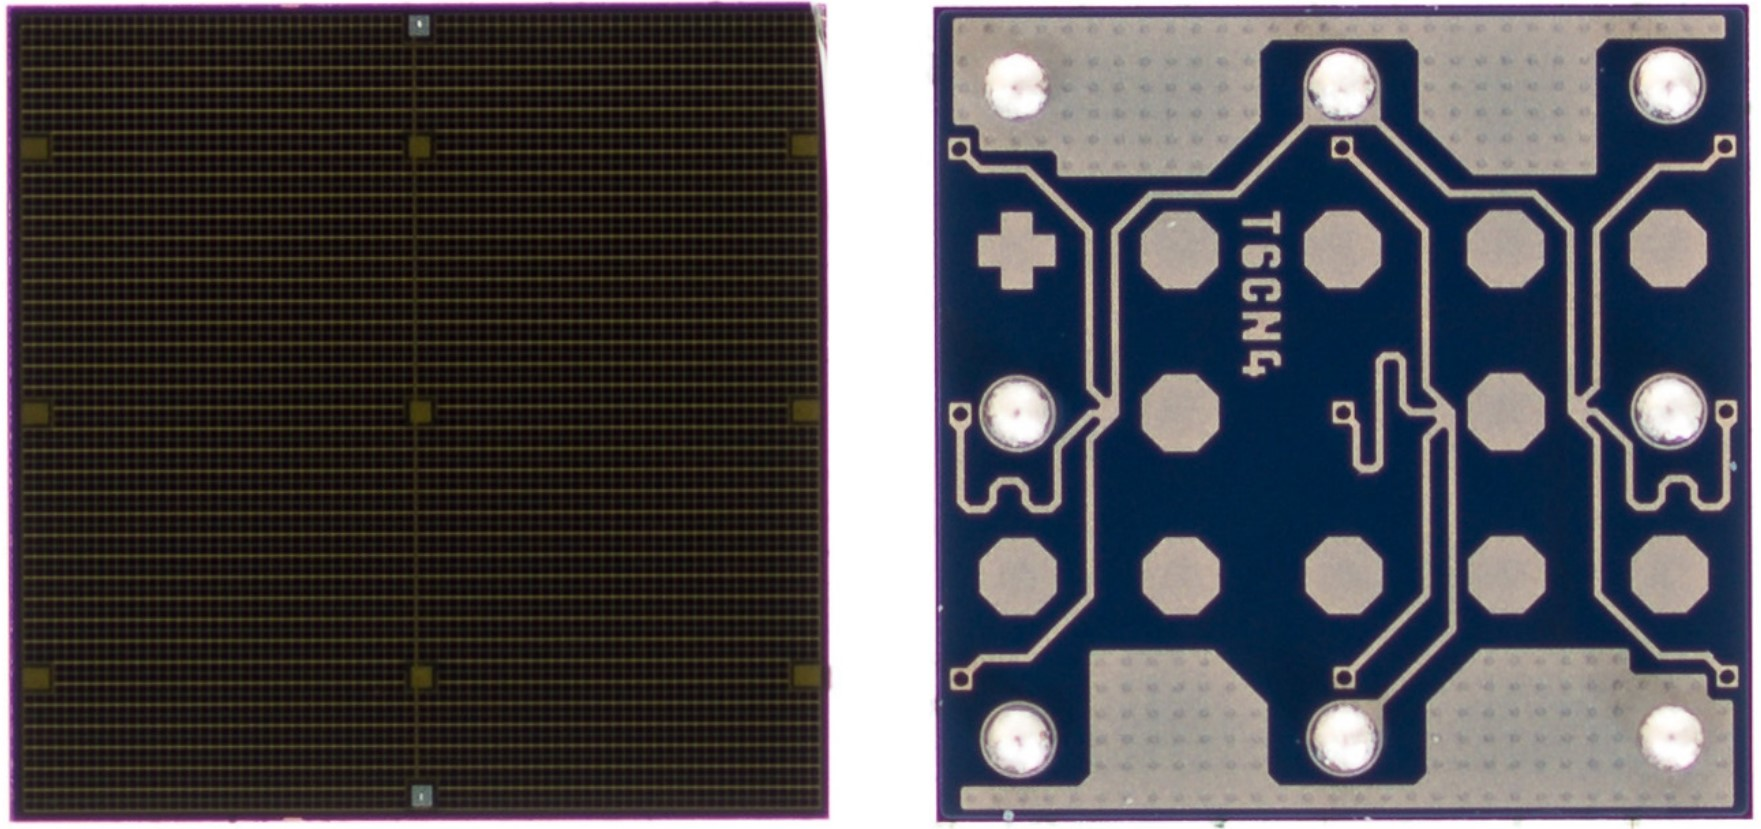
\includegraphics[width=0.8\textwidth]{detection_methods/MicroFJ−300XX−TSV.jpeg}
    \caption{Onsemi MicroFJ-300XX-TSV. Taken from \cite{Onsemi_SiPM}.}
    \label{fig:Onsemi_SiPM}
\end{figure}
\chapter{Electronics}
\label{chap:Electronics}

CosmicWatches have to be mainly low-cost and easy to build. In order to achieve this, the components selected for the construction have been carefully curated to make sure these restrictions were met. This however might be greatly responsible for some of the odd features found while testing the detector, like the lack of linearity and fluctuations in amplification and peak-detected values of seemingly equal input signals. The full KiCad project can be found in the GitHub repository: \href{https://github.com/anvargasl/CosmicWatch-gamma-spectroscopy-PCB}{CosmicWatch-gamma-spectroscopy-PCB}. The component numbers shown in this chapter are the ones that would have to be placed on the PCB in order to recreate the example schematics.

\begin{figure}[H]
    \centering
    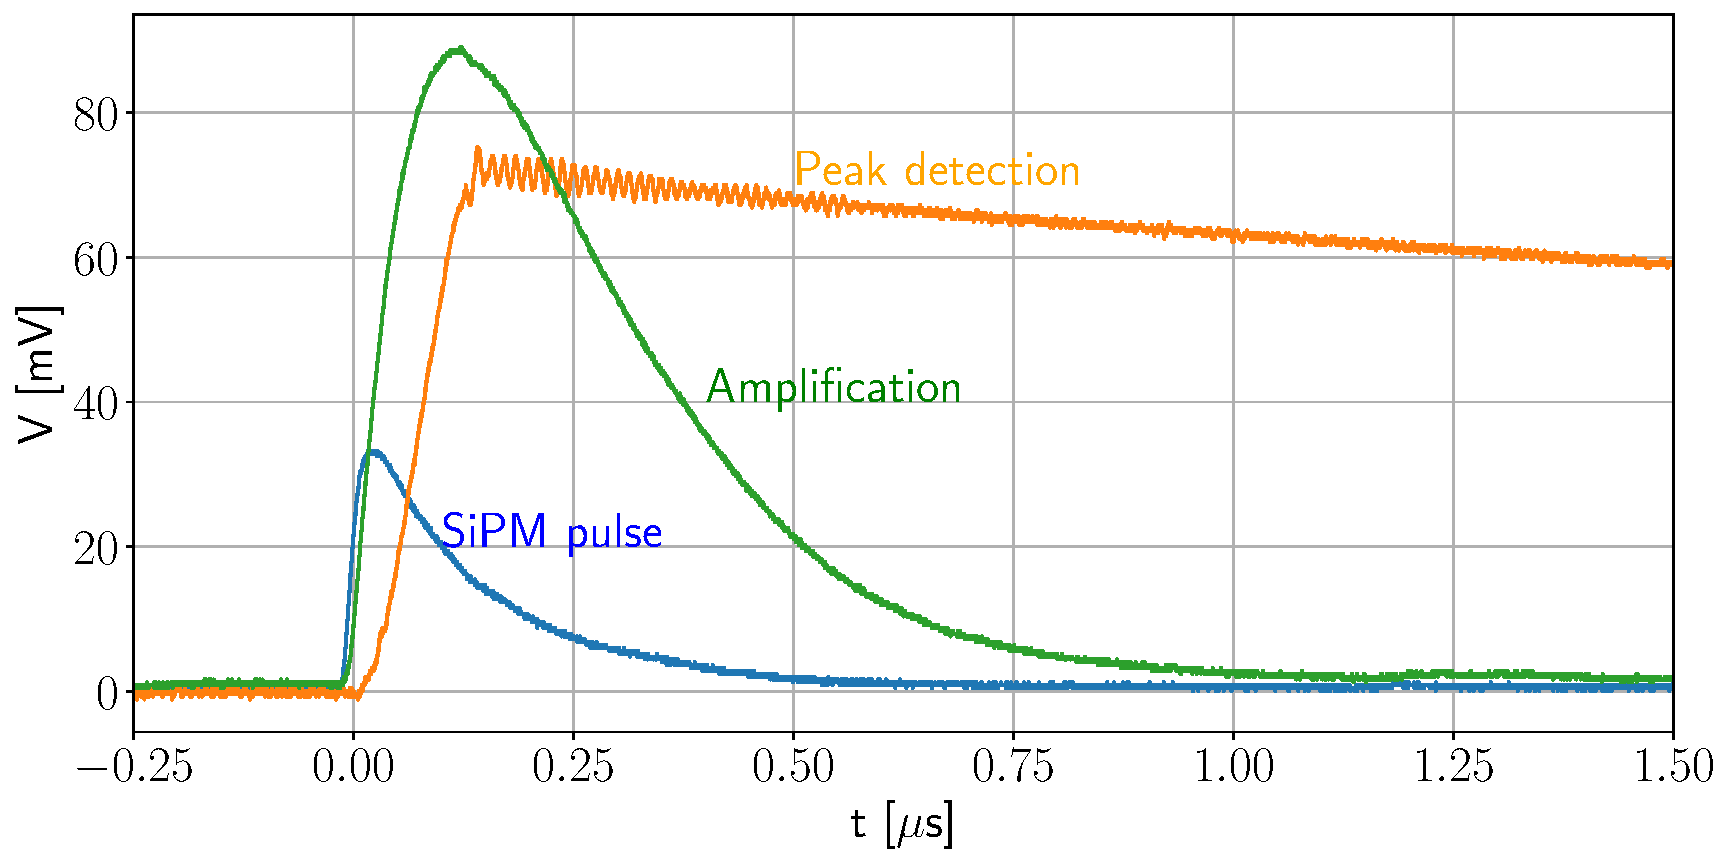
\includegraphics[width=0.8\textwidth]{Electronics/CW-signals.pdf}
    \caption{Signal processing inside the detector.}
    \label{fig:signal_processing}
\end{figure}

\section{Amplifier}

\begin{figure}[H]
    \centering
    \begin{circuitikz}[scale=0.7]
        \draw
        (0,0) node[op amp, noinv input up, font=\small] (opamp) {$U6$}
        (opamp.up) --++(0,0.5) node[vcc]{5\,\textnormal{V}}
        (opamp.down) --++(0,-0.5) node[vee]{-5\,\textnormal{V}}
        (opamp.+) node[left]{$V_{in}$}
        (opamp.-) node[left]{} to[short] ++(0, -3) coordinate(R4_R)
        to[R, l_=$R_4$] ++(-3, 0) node[ground]{}
        (R4_R) to[R, l_=$R_6$] ++(2.7, 0)
        %to[short] ++(0.1, 0) -|(opamp.out) to[short] ++(1, 0) node[ocirc, label={[yshift=0.3]$V_{out}$}]{}
        to[short] ++(0.1, 0) -|(opamp.out) to[short,-*] ++(1,0) node[above]{$V_{out}$};
        %to[short] ++(1, 0) node[ocirc, label=above:$V_{out}$]{};

        %Nodes
        %\node[shift={(0,+1.5)}] at (opamp) {U6 HLM6658};
    \end{circuitikz}
    \caption{Amplifier circuit schematic. An LT1807 op-amp is used for this and the peak detection stage.}
    \label{circ:amplifier}
\end{figure}

The processing of a pulse coming out of the SiPM has to go through two main stages, amplification and peak detection, Fig. \ref{fig:signal_processing} showcases these stages. The brightest SiPM pulses seen so far do not exceed 200 mV, which covers a very small portion of the ADC range on the RP Pico (0-3.3 V \cite[p.~18]{datasheet2024rp2040}). Amplification of the signal therefore allows for better resolution.

An op-amp on its own amplifies the voltage difference between the non-inverting (pin $+$) and inverting (pin $-$) inputs by its internal gain $A_{int}$, having then $V_{out}=A_{int}(V_+ - V_-)$. In this case, however, we are interested in controlling the gain of the circuit and therefore the amplification. In order to achieve this we introduce a feedback loop in the op-amp through $R4$ and $R6$, which controls how much of the output voltage is fed back into the op-amp. The theoretical amplification is therefore given by $V_{out}=(1+R6/R4)V_{in}$. A simple schematic showcasing the component arrangement is shown in Fig. \ref{circ:amplifier}.

\section{Peak Detector}

Since the LYSO crystal is so fast (36 ns of decay time \cite{Luxium_LYSO}) the ADC sample rate and response time of the Pico both play an important role in the number of events that the detector will accurately acquire. It is therefore necessary to hold the voltage of the amplified pulse in order to increase the chances of reading the actual value of the incoming signal. This is the task of the peak detector, to widen the time window in which we can sample the ADC and get a correct reading.

The idea behind the peak detector is to store charge in a capacitor ($C_{25}$) through a diode ($D_3$), retaining the highest voltage the input signal has reached. A diode is placed before the capacitor so that once the signal's voltage goes below the peak voltage, the diode will be reverse biased, therefore preventing current from flowing while maintaining the voltage on the capacitor.

In order to measure the voltage in the capacitor, a discharging resistor has to be added ($R_{15}/R_{19}$). The time it takes the capacitor to discharge is given by $t=RC$. Although for example in the case of CosmicWatch-V2's peak detector, the values of $R_{14}$ and $R_{24}$ also play a role in the discharging time, which has proved not to be as trivial as calculating the equivalent resistance $R_t$ of all three and simply take $t=R_tC$.

The schematic and PCB shown in the repository \href{https://github.com/anvargasl/CosmicWatch-gamma-spectroscopy-PCB}{CosmicWatch-gamma-spectroscopy-PCB}, include the connections and footprints necessary to place the components that make the designs illustrated in Subsections \labelcref{sec:basic,sec:pd_V2,sec:basic_buffer,sec:nuclear_phoenix}. Different results were found while testing these peak detector setups.

\subsection{Basic Peak Detector}\label{sec:basic}

\begin{figure}[H]
    \centering
    \begin{circuitikz}[scale=0.7]
        %\draw [help lines] (-4,0) grid (5,-4);
        \draw (0,0) node[op amp, noinv input up, font=\small] (opamp) {$U6$}
        (opamp.up) --++(0,0.5) node[vcc]{5\,\textnormal{V}}
        (opamp.down) --++(0,-0.5) node[vee]{-5\,\textnormal{V}}
        (opamp.+) node[left]{$V_{in}$}
        (opamp.out) node[]{} to[sD, l_=$D_3$] (6, 0) coordinate (D3_r)
        (opamp.-) node[left]{} to[short] ++(0, -2.5) coordinate (R24_l)
        (R24_l) to[R, l^=$R_{24}$, resistors/scale=0.8] (D3_r |- , |- R24_l) coordinate (R24_r)
        (D3_r) -- (R24_r)
        (D3_r) -- ++(1,0) coordinate (C25_u)
        (C25_u) to[C, l=$C_{25}$] ++(0,-2) node[ground]{}
        (C25_u) -- ++(2,0) to[R, l=$R_{15}$, resistors/scale=0.8] ++(0,-2) node[ground]{};
        %\draw (A |- 52,3)(D3_r) -- (R24_r);
        % to[short] ++(-0.1, 0) -|(R24_r)
    \end{circuitikz}
    \caption{Basic peak detector design.}
    \label{circ:basic_pd}
\end{figure}

Assuming ideal conditions, a diode is enough to retain the highest input voltage reached. Semiconductor diodes however don't behave ideally, they introduce a voltage drop that will keep the voltage stored in $C_{25}$ at a lower potential than that of $V_{in}$. In order to prevent this, an op-amp $(U_6)$\footnote{Currently the only op-amp that has behaved reasonably well is the LT1807 by Analog Devices Inc. The LMH6658  by Texas Instruments seems to have trouble driving even small capacitors.} is placed before the diode. In the configuration shown in Fig. \ref{circ:basic_pd}, the opamp will try to output the necessary current to equilibrate the inverting input voltage (pin $-$) to what it sees in the non-inverting input (pin $+$), to achieve this $U_6$ has to go one diode drop above $V_{in}$.

\subsection{Preventing negative saturation}\label{sec:pd_V2}

\begin{figure}[H]
    \centering
    \begin{circuitikz}[scale=0.7]
        %\draw [help lines] (-4,0) grid (5,-4);
        \draw (0,0) node[op amp, noinv input up, font=\small] (opamp) {$U_6$}
        (opamp.up) --++(0,0.5) node[vcc]{5\,\textnormal{V}}
        (opamp.down) --++(0,-0.5) node[vee]{-5\,\textnormal{V}}
        (opamp.+) node[left]{$V_{in}$}
        (opamp.out) -- ++(1,0) coordinate(oa_out) to[sD, l_=$D_3$] (6, 0) coordinate (D3_r)
        (opamp.-) -- ++(0, -2.7) coordinate (ver_1) -- ++(1, 0) coordinate(D5_l)
        (ver_1) to[R, l_=$R_{14}$, resistors/scale=0.8] ++(-2,0) node[ground]{} 
        (D5_l) to[sD, l_=$D_5$] (oa_out |- , |- D5_l) coordinate (D5_r)
        (oa_out) -- (D5_r)
        (D5_l) -- ++(0,-1.7) coordinate (R24_l)
        (R24_l) to[R, l^=$R_{24}$, resistors/scale=0.8] (D3_r |- , |- R24_l) coordinate (R24_r)
        (D3_r) -- (R24_r)
        (D3_r) -- ++(1,0) coordinate (C25_u)
        (C25_u) to[C, l=$C_{25}$] ++(0,-2) node[ground]{}
        (C25_u) -- ++(2,0) to[R, l=$R_{15}$, resistors/scale=0.8] ++(0,-2) node[ground]{};
    \end{circuitikz}
    \caption{Basic peak detector design, a second diode is added in order to prevent the op-amp from entering a negative saturation loop.}
    \label{circ:pd_V2}
\end{figure}

In the basic peak detector, once the signal voltage goes below the peak voltage, $D_3$ will be reverse biased and the inverting input of the opamp will see a higher voltage than the non-inverting input, this will force $U_6$ to go into negative saturation by driving the output voltage as low as it can in order to match both inputs. Once the signal gets close to the stored voltage in $C_25$, the op-amp will have to get out of the negative saturation, this will take some time which depends on the slew rate of the opamp and therefore limits the operating frequency range of the circuit.

In order to avoid negative saturation $D_5$ is added, along with an outer feedback loop through $R_{24}$. In this case, once the input signal goes below the stored voltage, $D_5$ will be forward biased, allowing for a new feedback loop that decreases the op-amp's negative saturation time.


\subsection{Basic Peak Detector + Buffer}\label{sec:basic_buffer}

\begin{figure}[H]
    \centering
    \begin{circuitikz}[scale=0.7]
        %\draw [help lines] (-4,0) grid (5,-4);
        \draw (0,0) node[op amp, noinv input up, font=\small] (opamp) {$U_6$}
        (opamp.up) --++(0,0.5) node[vcc]{5\,\textnormal{V}}
        (opamp.down) --++(0,-0.5) node[vee]{-5\,\textnormal{V}}
        (opamp.+) node[left]{$V_{in}$}
        (opamp.out) -- ++(1,0) coordinate(oa_out) to[sD, l_=$D_3$] (6, 0) coordinate (D3_r)
        (opamp.-) -- ++(0, -2.7) coordinate (ver_1) -- ++(1, 0) coordinate(D5_l)
        (ver_1) to[R, l_=$R_{14}$, resistors/scale=0.8] ++(-2,0) node[ground]{} 
        (D5_l) to[sD, l_=$D_5$] (oa_out |- , |- D5_l) coordinate (D5_r)
        (oa_out) -- (D5_r)
        (D5_l) -- ++(0,-1.7) coordinate (R24_l)
        (D3_r) -- ++(1,0) coordinate (C25_u)
        (C25_u) to[C, l=$C_{25}$] ++(0,-2) node[ground]{}
        (C25_u) -- ++(2,0) coordinate (buffer_l)
        (buffer_l) node[op amp, noinv input up, font=\small, anchor=+] (buffer) {$U_7$}
        (buffer.-) coordinate (buffer_-)
        (buffer.out) coordinate (buffer_out)
        (buffer_-) -- (buffer_- |-, |- R24_l) coordinate (R24_r)
        (R24_l) to[R, l^=$R_{24}$, resistors/scale=0.8] (R24_r)
        (R24_r) -- (buffer_out |-, |- R24_r) -- (buffer_out)
        (buffer_out) to[short, -*] ++(1,0);
        %(D3_r) -- (R24_r);
        %(C25_u) -- ++(2,0) to[R, l=$R_{15}$, resistors/scale=0.8] ++(0,-2) node[ground]{};
    \end{circuitikz}
    \caption{Basic peak detector design, Adding a buffer to prevent discharging of the capacitor through the resistor and instead through any load in the circuit, in this case $R_{29}$.}
    \label{circ:pd_buffer}
\end{figure}

This design follows the same principles as the one shown in the previous subsection. However, in this case, a buffer is added to introduce high impedance and prevent the capacitor from discharging through the resistor and instead through any load that may be applied after the circuit.

\subsection{Nuclear Phoenix}\label{sec:nuclear_phoenix}

\begin{figure}[H]
    \centering
    \begin{circuitikz}[scale=0.7]
        %\draw [help lines] (-4,0) grid (5,-4);
        \draw (0,0) node[op amp, noinv input up, font=\small] (opamp) {$U_6$}
        (opamp.up) --++(0,0.5) node[vcc]{5\,\textnormal{V}}
        (opamp.down) --++(0,-0.5) node[vee]{-5\,\textnormal{V}}
        (opamp.+) node[left]{$V_{in}$}
        (opamp.out) coordinate(oa_out) to[sD, l_=$D_5$] ++(2, 0) coordinate (D5_r)
        (D5_r) to[sD, l_=$D_3$] ++(2, 0) coordinate (D3_r)
        (D5_r) -- ++(0,-4) coordinate (R30_l)
        (D3_r) -- ++(3,0) coordinate (C25_u)
        (C25_u) to[C, l=$C_{25}$] ++(0,-2) node[ground]{}
        (C25_u) -- ++(2,0) coordinate (buffer_l)
        (opamp.-) coordinate (oa_-)
        (oa_-) -- ++(-1.5, 0) -- ++(0, 4) coordinate(aux1)
        (aux1) -- (D3_r |-, |- aux1) -- (D3_r)
        (buffer_l) node[op amp, noinv input up, font=\small, anchor=+] (buffer) {$U_7$}
        (buffer.-) coordinate (buffer_-)
        (buffer.out) coordinate (buffer_out)
        (buffer_-) -- (buffer_- |-, |- R30_l) coordinate (R30_r)
        (R30_l) to[R, l_=$R_{30}$, resistors/scale=0.8] (R30_r)
        (R30_r) -- (buffer_out |-, |- R30_r) -- (buffer_out)
        (buffer_out) to[short, -*] ++(1,0);
        %(D3_r) -- (R24_r);
        %(C25_u) -- ++(2,0) to[R, l=$R_{15}$, resistors/scale=0.8] ++(0,-2) node[ground]{};
    \end{circuitikz}
    \caption{Nuclear Phoenix peak-detector design. Taken from \cite{Nucelar_phoenix}.}
    \label{circ:pd_np}
\end{figure}

NuclearPhoenix is a physics student who has developed a gamma detector that also utilizes a Raspberry Pi Pico and a Silicon photomultiplier, his schematics also include a peak detection circuit which is shown in Fig. \ref{circ:pd_np}, his project can be found in \href{https://nuclearphoenix.xyz/hardware/ogd/}{Open Gamma Detector}. This design aims to prevent leakage current across $D_3$, this discharges the capacitor at a faster rate than intended once the peak voltage has been reached. In this case, $R_30$ is feeding back the peak voltage value to $D_3$, therefore creating a 0 V difference across the diode, preventing any leakage current from flowing out of $C_{25}$ and into the output of the op-amp.

\section{Trigger}

\begin{figure}[H]
    \centering
    \begin{circuitikz}[scale=0.7]
        %\draw [help lines] (-4,0) grid (5,-4);
        \draw (0,0) node[op amp, noinv input up, font=\small] (opamp) {$U_6$}
        (opamp.up) --++(0,0.5) node[vcc]{5\,\textnormal{V}}
        (opamp.down) --++(0,-0.5) node[vee]{-5\,\textnormal{V}}
        (opamp.out) --++(1,0) node[above]{$V_{out}$}
        (opamp.+) node[left]{$V_{in}$}
        (opamp.-) --++(-2.5,0)  coordinate (oa_-)
        (oa_-) to[R, l^=$R_{16}$, resistors/scale=0.8] ++(0,2) to[R, l^=$R_{22}$, resistors/scale=0.8] ++(0,2) node[vcc]{5\,\textnormal{V}}
        (oa_-) to[R, l_=$R_{18}$, resistors/scale=0.8] ++(0,-2) node[ground]{};

        %Nodes
        \node[shift={(-0.3,-0.3)}] at (opamp.-) {$V_{REF}$};
    \end{circuitikz}
    \caption{Trigger circuit.}
    \label{circ:trigger}
\end{figure}

In this case, a voltage divider is used to force a positive saturation in the op-amp once the amplified signal reaches a threshold voltage, generating a "digital 1"\: that can be used to trigger the detector. The threshold, or $V_{REF}$ as noted in Fig. \ref{circ:trigger}, is given by equation \eqref{eq:v_ref}.

\begin{equation}
    V_{REF}=\frac{R_{18}}{R_{22}+R_{16}+R_{18}} V_{cc} \label{eq:v_ref}
\end{equation}

%add code as appendix
\section{Microcontroller}

\section{DC to DC booster}

\begin{figure}[H]
    \centering
    \begin{circuitikz}
        % U1 NE555
        \draw [thick] (0,0) coordinate (u1) rectangle ++(2,3); % shape
        \draw [pin] (u1) ++(1, 3.8)
            node[]{$U_1$};
        \draw [pin] (u1) ++(1, 3.3)
            node[]{MAX5026};
        %-----------Left side-----------%
        \draw [pin] (u1) ++ (0,2.5) coordinate (u1 pgnd)
            node[right, font=\scriptsize]{PGND}
            node[above left]{1}; % CON
        \draw [pin] (u1) ++ (0,1.5) coordinate (u1 gnd)
            node[right, font=\scriptsize]{GND}
            node[above left]{2}; % TRI
        \draw [pin] (u1) ++ (0,0.5) coordinate (u1 fb)
            node[right, font=\scriptsize]{FB}
            node[above left]{3}; % THR
        
        %-----------Right side-----------%
        \draw [pin] (u1) ++ (2,2.5) coordinate (u1 lx)
            node[left, font=\scriptsize]{LX}
            node[above right]{6}; % OUT
        \draw [pin] (u1) ++ (2,1.5) coordinate (u1 vcc)
            node[left, font=\scriptsize]{VCC}
            node[above right]{5}; % OUT
        \draw [pin] (u1) ++ (2,0.5) coordinate (u1 shdn)
            node[left, font=\scriptsize]{SHDN}
            node[above right]{4}; % OUT
        %\draw (u1) ++ (2,0)
        %    node[right]{\ctikzlabel{$U_1$}{NE555}}; % NE555P
        
        % U1 NE555 Pins
        \draw (u1 pgnd) -- ++ (-1,0) node[ground]{}; % PGND

        \draw (u1 gnd) -- ++ (-1,0) node[ground]{}; % GND

        \draw (u1 fb) -- ++ (-2,0) coordinate(r10 u) to[R, l_=$R_{10}$, resistors/scale=0.8] ++(0,-2) node[ground]{}
        (r10 u) to[R, l^=$R_{2}$, resistors/scale=0.8] ++(0,2) -- ++(0,2) -- ++(7,0) coordinate(d4 r)
        (d4 r) --++(2,0) coordinate(c3 u) to[R, l^=$R_{25}$, resistors/scale=0.8] ++(2,0) coordinate (c4 u)
        (c3 u) to[C, l_=$C_{3}$, resistors/scale=0.8] ++(0,-2)  node[ground]{}
        (c4 u) to[C, l_=$C_{4}$, resistors/scale=0.8] ++(0,-2)  node[ground]{}
        (c4 u) --++(1,0) node[vcc]{\textnormal{HV}}; % FB

        \draw (u1 lx) -- ++ (1,0) coordinate(d4 l)
        (d4 l) -- ++(0,1) to[sD, l^=$D_3$] ($(d4 r) + (0,-1)$) -- (d4 r)
        (d4 l) to[american inductor, l_=$L_1$] ($(d4 r) + (0,-2)$) coordinate(l1 r); % LX

        \draw (u1 vcc) -- ++ (1,0) to[short, -*] ++(0,-1); % VCC

        \draw (u1 shdn) --++(2,0) coordinate(c7 u) --++(1,0) coordinate (c2 u) --(l1 r)
        (c7 u) to[C, l_=$C_{7}$, resistors/scale=0.8] ++(0,-2) node[ground]{}
        (c2 u) to[C, l=$C_{2}$, resistors/scale=0.8] ++(0,-2) node[ground]{}
        (c2 u) --++(1,0) node[vcc]{5\,\textnormal{V}}; % SHDN
    \end{circuitikz}
    \caption{DC to DC booster circuit. Careful considerations have to be made when placing the MAX5026 IC in order to reduce noise on the power line. It is advised to have a look at the datasheet in \cite{AnalogDevices_DC_DC}, section "Applications Information".}
    \label{circ:booster}
\end{figure}

Acording to Onsemi \cite{Onsemi_SiPM}, the operaing voltage of a MicroFJ-300XX-TSV SiPM is 25.2-30.7 V. It is then necessary to boost $V_{cc}$ to the operating range of the SiPM, noted as HV in Fig. \ref{circ:booster}. In order to achive this, a MAX5026 PWM Step-Up DC-DC Converter is used \cite{AnalogDevices_DC_DC}, which has a user-adjustable output voltage of up to 36 V using external feedback resistors.

In the circuit shown in Fig. \ref{circ:booster}, $R_{10}$ and $R_2$ determine the output voltage HV. According to \cite{AnalogDevices_DC_DC}, equation \eqref{eq:booster_fb_resistance} allows to calculate the Value of $R_{10}$ given a desired output voltage HV and a value of $R_2$ between 5 and 50 \unit{\kilo\ohm}.

\begin{equation}
    R_{10} = R_2\left(\frac{\text{HV}}{V_{REF}}-1\right) \label{eq:booster_fb_resistance}
\end{equation}

\section{Single photons}
\chapter{Geant4 Simulations}

In order to provide a new interactive approach to CosmicWatches for new users a scintillation simulation has been devised using the Geant4 toolkit. With this, we intend to showcase some of the physical aspects that may be studied with the detector. This project is still in development and can be found on the GitHub repository \href{https://github.com/spenceraxani/CosmicWatch_Geant4}{CosmicWatch\_Geant4}. This section aims to give a brief explanation of the inner workings of the simulation as well as the Geant4 toolkit.

\section{What is Geant4?}

As defined by the authors \cite{Geant4}, Geant4 is a simulation toolkit based in \texttt{C++}, to model the passage of particles through matter, allowing the creation of custom detector geometries, tracking, and hit recollection, it includes multiple physics models for processes covering a wide range of specialties, such as electromagnetic, hadronic, and optical processes. Its main areas of application are high energy, nuclear, and accelerator physics, as well as medical and space science.

A comprehensive \href{https://geant4-userdoc.web.cern.ch/UsersGuides/InstallationGuide/html/}{installation guide} has been made by the authors, the toolkit is available on Windows, MacOS, and Linux. We recommend building and installing it from source using CMake, since it provides great control over the specific configurations available during installation. Some great tutorials can also be found online, the simulations shown here are based on the architecture illustrated by Physics Matters in his YouTube series \href{https://youtube.com/playlist?list=PLLybgCU6QCGWgzNYOV0SKen9vqg4KXeVL&si=mdzOyTZS0DYsf_vc}{Geant4 Tutorials}.

\section{Geometry}

As noted before, Geant4 allows the creation of custom geometries, which in our use case is great, since it provides a platform suitable for testing multiple CosmicWatch configurations as shown in Sections \labelcref{sec:collected_produced,sec:SiPM_placement,sec:Scint_size,sec:cos_squared}.

In general, Geant4 requires a mother volume in which the simulation will take place, in this case, we have chosen a $20\times20\times20$ \unit{\cm\cubed} box of \texttt{G4\_AIR}\footnote{This and all other materials used in the simulation, are built from the \textit{Geant4 Material Database}, accessed through the \texttt{G4NistManager} class}. The scintillating material is a $5\times5\times1$ \unit{\cm\cubed} box. The sizes of all these elements can of course be changed (as explored in Section \labelcref{sec:Scint_size}) the settings detailed above are just the default configuration in \texttt{headers/construction.hh}. Fig. TALES shows the SiPM and scintillator placement inside the mother volume.

%----------------include detector geometry screenshot

For simplicity, the SiPM is also modeled as a box filled with \texttt{G4\_AIR} with dimensions $3\times3\times1$ \unit{\mm\cubed}. The detected photons specified in the following subsections are counted as they enter the SiPM volume, this volume-check process is done in \texttt{source/stepAction.cc}, and relevant information for every event is saved to a \texttt{ntuple} by the \texttt{G4GenericAnalysisManager} class as defined in \texttt{source/eventAction.cc}. The simulation speed could be improved by employing the \text{G4VHits} and \texttt{G4THitsCollection} classes, which are optimized to record data for every step inside a sensitive volume in the simulation.

As discussed in \labelcref{sec:self_radiation}, LYSO crystals contain $^{176}$Lu, a naturally occurring radioactive isotope emitting betas. LYSO crystals can absorb their own radiation, resulting in a constant background, this feature however, has not yet been included in the simulation, which is why the scintillating material used is the same as in previous versions of CosmicWatch, a plastic scintillator based on Polyvinyltoluene, the material name in the \textit{Geant4 Material Database} is \texttt{G4\_PLASTIC\_SC\_VINYLTOLUENE}.

\section{Muons going through the scintillator}

The following simulation results were thought to recreate some of the results typically seen with CosmicWatches, they also give insight into some construction characteristics that can be taken into account while building a detector. In order to speed up the simulation the muons being shot by the simulation have initial energies of 50 \unit{\mega\eV}, much lower to what would be expected at sea level (4 \unit{\giga\eV}). The particle gun used in this simulation is a \texttt{G4GeneralParticleSource}, the setting of this particle gun can be changed in macro files. Figures TALES show some of the geometries the particle source can have.

\section{Simulation results}

\subsection{Photons collected vs. produced}\label{sec:collected_produced}

\subsection{SiPM placement}\label{sec:SiPM_placement}

The collocation of the SiPM can be a factor to keep in mind while designing new CosmicWatch setups. Generally, the photomultiplier is located on the base of the scintillator as shown in Figure TALES, but it may be useful to place it on one of its sides as shown in Fig. TALES.

\begin{figure}[H]
    \centering
    \begin{subfigure}[t]{0.48\textwidth}
      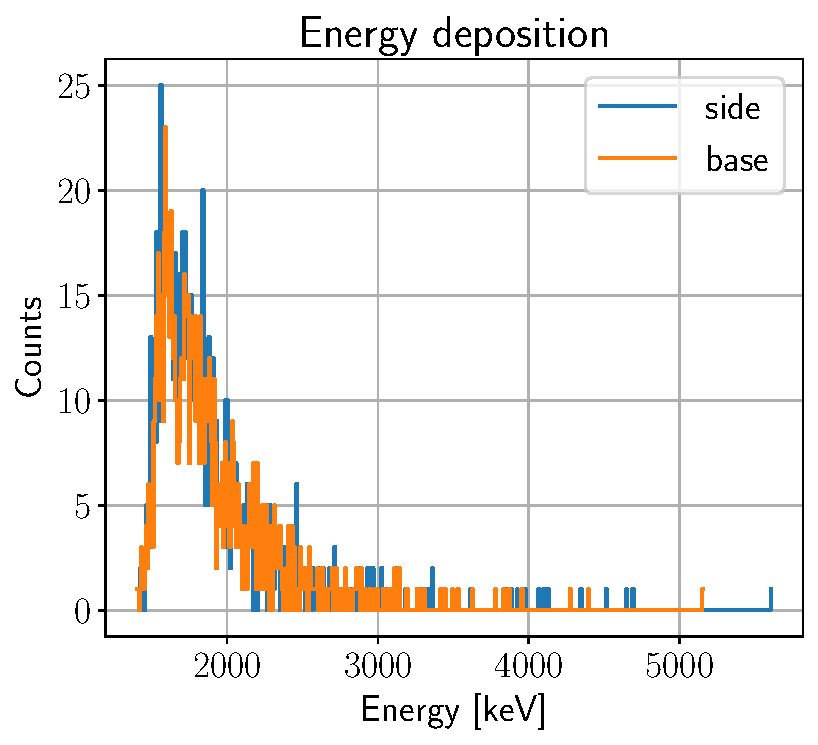
\includegraphics[width=\textwidth]{G4_simulations/run0_nt_Event_SiPM-placement_energy_spectra.pdf}
      \caption{\label{sfig:SiPM_place_edep}Energy deposition in the detector for different photomultiplier placements.}
    \end{subfigure}
    \hfill
    \begin{subfigure}[t]{0.48\textwidth}
      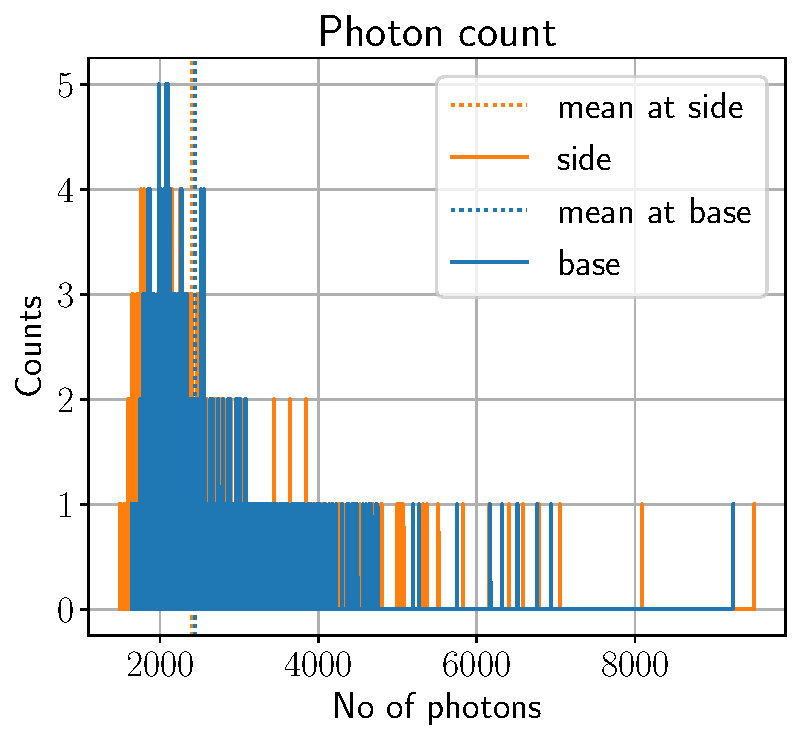
\includegraphics[width=\textwidth]{G4_simulations/run0_nt_Event_SiPM-placement_photon_count.pdf}
      \caption{\label{sfig:SiPM_place_pcount}SiPM photon count for both setups.}
    \end{subfigure}
    \caption{\label{fig:SiPM_place_results}The SiPM placement can be easily changed in the simulation by choosing between \texttt{base} and \texttt{side} as values for the construction variable \texttt{SiPMpos} in \texttt{headers/construction.hh}.}
\end{figure}

As expected, the energy deposition in the crystal should not depend on the SiPM placement. Surprisingly enough, however, it seems that the photon count is also not affected by this, meaning that the results obtained with both setups should be similar while using the specified scintillator size.

\subsection{Scintillator sizes}\label{sec:Scint_size}

The current architecture of CosmicWatch allows to use of variable scintillator sizes, the first versions of CosmicWatch used 5$\times$5$\times$1 \unit{\cm\cubed} scintillators, while the newer LYSO crystals are much smaller Fig. TALES shows some of the crystals used while testing the detector response.

\begin{figure}[H]
  \centering
  \begin{subfigure}[t]{0.48\textwidth}
    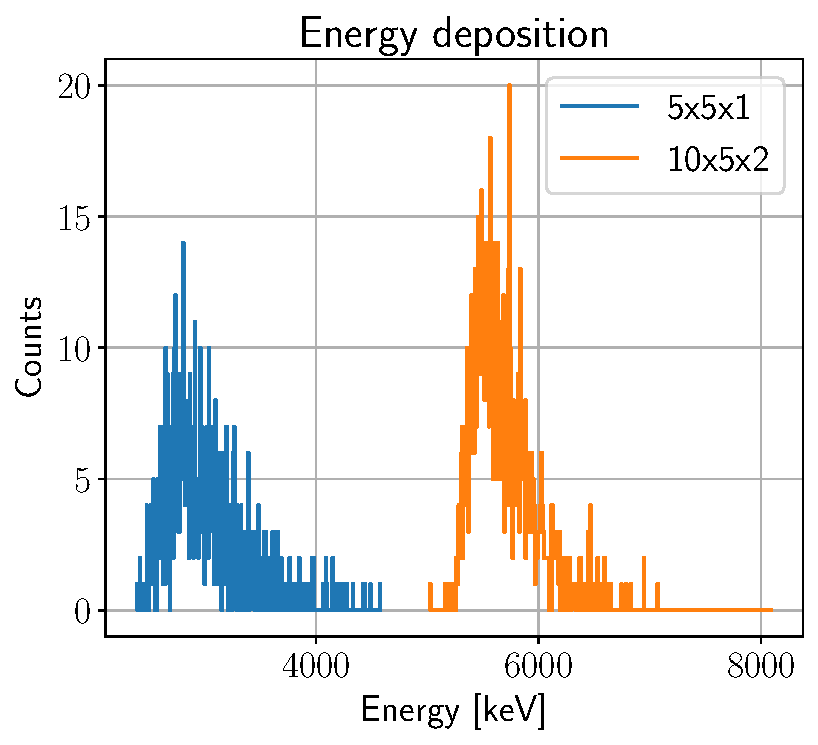
\includegraphics[width=\textwidth]{G4_simulations/run0_nt_Event_crystal-size_energy_spectra.pdf}
    \caption{\label{sfig:scint_size_edep}Energy deposition in the detector for different scintillator sizes.}
  \end{subfigure}
  \hfill
  \begin{subfigure}[t]{0.48\textwidth}
    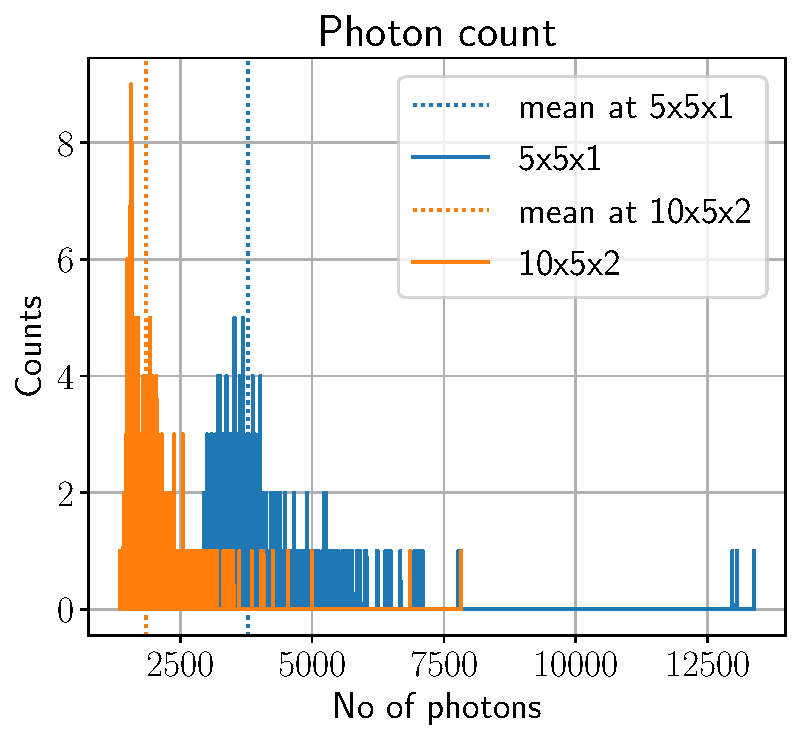
\includegraphics[width=\textwidth]{G4_simulations/run0_nt_Event_crystal-size_photon_count.pdf}
    \caption{\label{sfig:scint_size_pcount}SiPM photon count for different scintillator sizes.}
  \end{subfigure}
  \caption{\label{fig:scint_size_results}The scintillator size can be easily chosen inside the simulation by changing the values of \texttt{PScintXBase}, \texttt{PScintYBase}, and \texttt{PScintHeigh} in \texttt{headers/construction.hh}.}
\end{figure}

Figure \ref{sfig:scint_size_edep} shows that bigger SiPM sizes do result in greater energy recollections, however, as Figure \ref{sfig:scint_size_pcount} illustrates, the number of photons that reached the SiPM was on average greater for the $5\times5\times1$ \unit{\cm\cubed} setup. These figures then show that increased scintillator volume does not directly correlate with photon counts in the SiPM, which is ultimately the goal of the detector, to collect as many photons as possible in the photomultiplier to increase energy resolution.

\subsection{Angular distributions}\label{sec:cos_squared}

With this simulation, we are trying to understand the detector response as a function of the zenith angle $\theta$, studying the energy deposition in the scintillating material and photon count in the SiPM depending on the trajectory of the particle once it enters the detector. As shown in Figure TALES, a spherical particle source was used to shoot particles from all directions toward the center of the scintillating crystal. This however, does not recreate the cosine squared law, as the particle source is ``isotropic,'' meaning that it does not have a preferred direction to shoot particles from.

\begin{figure}[H]
  \centering
  \begin{subfigure}[t]{0.48\textwidth}
    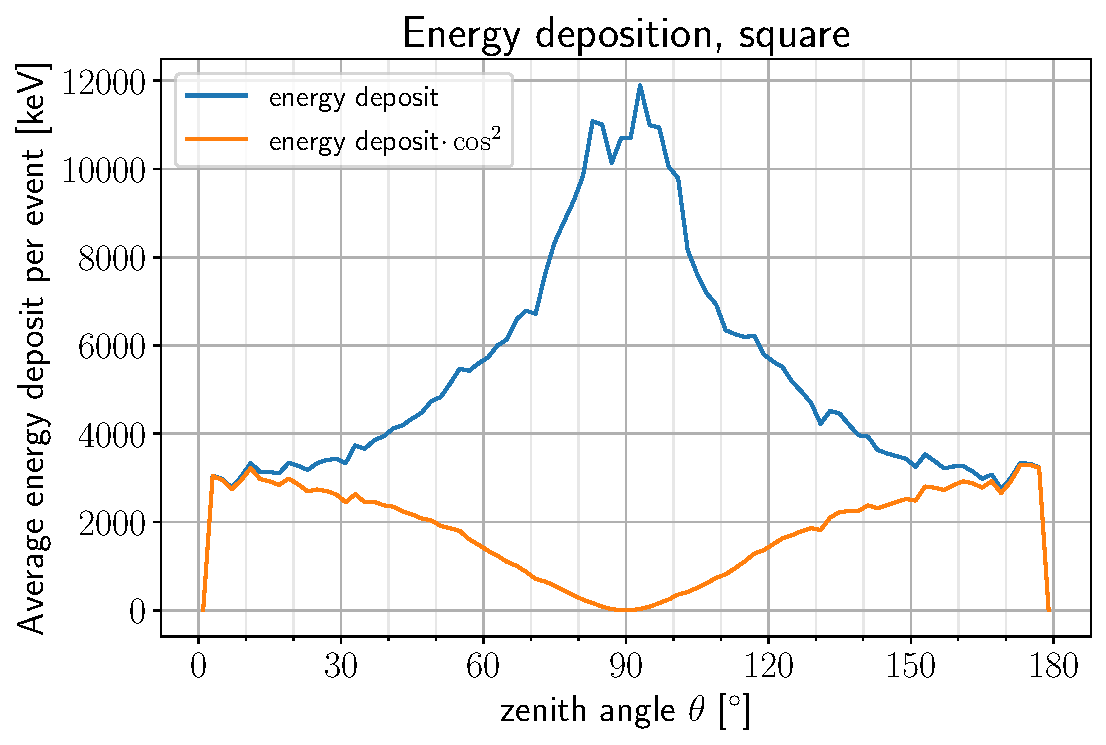
\includegraphics[width=\textwidth]{G4_simulations/run0-ang_dis_nt_Event_energy_spectra.pdf}
    \caption{\label{sfig:ang_edep}Energy deposition in the detector as a function of zenith angle.}
  \end{subfigure}
  \hfill
  \begin{subfigure}[t]{0.48\textwidth}
    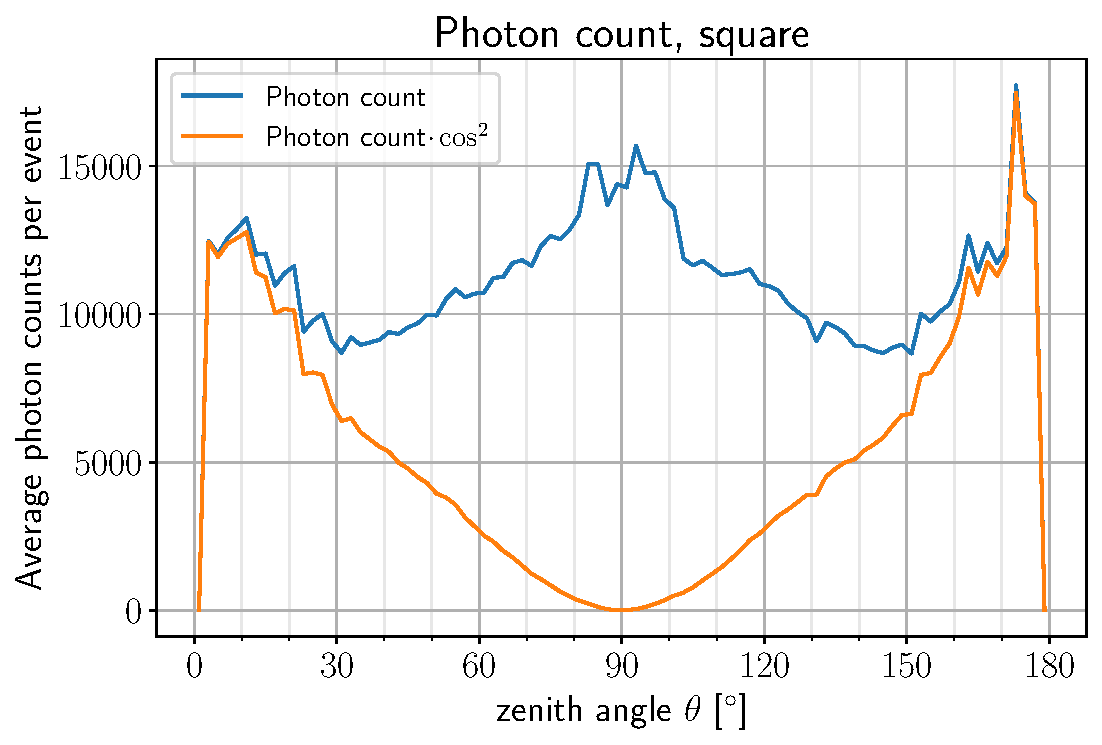
\includegraphics[width=\textwidth]{G4_simulations/run0-ang_dis_nt_Event_photon_count.pdf}
    \caption{\label{sfig:ang_pcount}SiPM photon as a function of zenith angle.}
  \end{subfigure}
  \medskip
  \begin{subfigure}[t]{0.48\textwidth}
    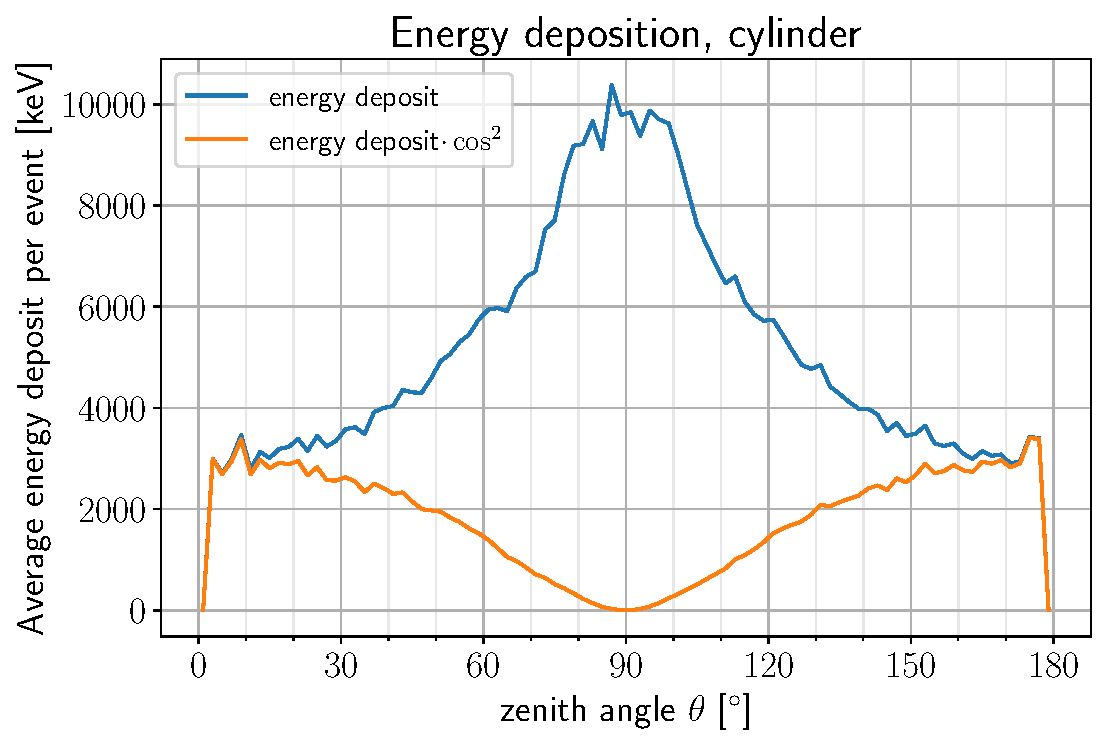
\includegraphics[width=\textwidth]{G4_simulations/test_nt_Event_energy_spectra.pdf}
    \caption{\label{sfig:ang_edep_cylinder}Energy deposition in the detector as a function of zenith angle with a cylindrical scintillator.}
  \end{subfigure}
  \hfill
  \begin{subfigure}[t]{0.48\textwidth}
    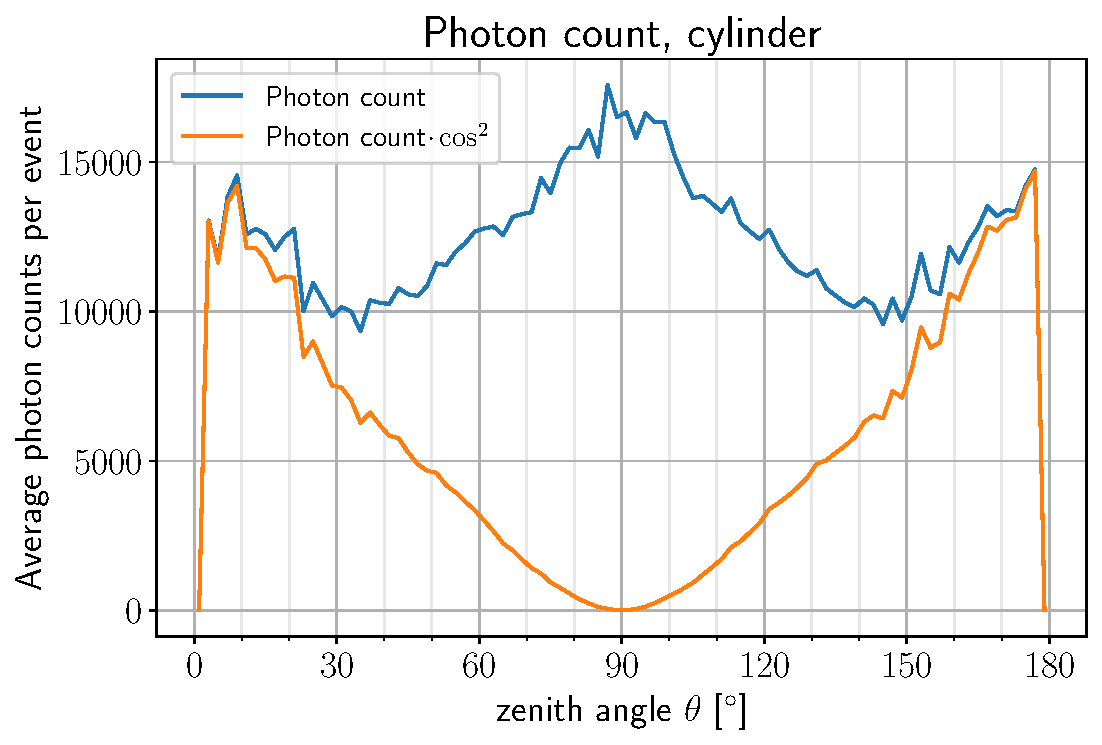
\includegraphics[width=\textwidth]{G4_simulations/test_nt_Event_photon_count.pdf}
    \caption{\label{sfig:ang_pcount_cylinder}SiPM photon as a function of zenith angle with a cylindrical scintillator.}
  \end{subfigure}
  \caption{\label{fig:ang_results}Data in blue is the raw output of the simulation while shooting muons directly toward the center of the scintillator. Data in orange is the normalization of the simulation output using a cosine squared law.}
\end{figure}

As can be seen in Figure TALES, muons traveling directly downward have less scintillating material to go through compared to those traveling horizontally, this means that greater zenith angles should result in greater energy depositions, which agrees with the data shown in Figures \ref{sfig:ang_edep} and \subref{sfig:ang_edep_cylinder}. In Figure \ref{sfig:ang_pcount} however, the photon count first decreases to a minimum at around 30$^\circ$ to then steadily increase until 90$^\circ$. Based on what we learned in the previous section \ref{sec:Scint_size} about scintillator sizes, and keeping in mind the detector geometry, one would expect a minimum photon count at the angle where the photons have to travel the greatest distance, which in this case corresponds the scintillator edges an corners, ranging between 78.69 and 81.95 degrees for a $5\times5\times1$ \unit{\cm\cubed} scintillator.

In order to attenuate any possible polar dependencies, the scintillator geometry was changed to a cylinder as shown in Figure TALES. This however, does not seem to have a correlation with the presence of a minimum in photon count at 30$^\circ$, as can be seen in Figure \ref{sfig:ang_pcount_cylinder}.

\subsection{Simulated Spectra}
\chapter{Measurements}\label{chap:measurements}

In order to test the detector and crystal response, multiple electronic setups were used to obtain spectra from calibrated sources. This chapter summarizes the most important measurements achieved while testing the CosmicWatch, showcasing some features that are yet to be understood. It is important to note that for every measured spectrum a background radiation measurement was also performed and all calibrations were made while subtracting the background. In the plots, sometimes the background is presented to showcase the counts of a spectrum relative to it, when the background is not included in the plot it means that it has been subtracted from that specific spectrum.

\section{CosmicWatch electronics}\label{sec:CW_measurements}

\subsection{ADC shortcomings}\label{sec:ADC_shortcomings}

\subsubsection{Resolution}

\begin{figure}
  \centering
  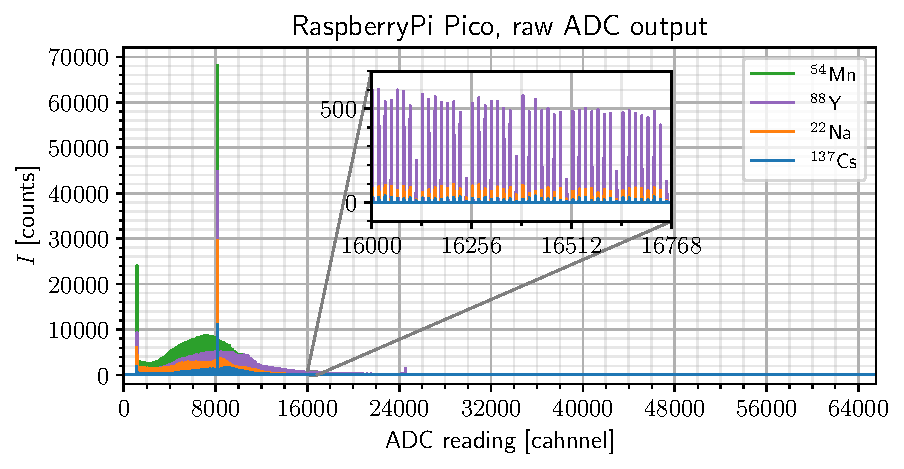
\includegraphics[width=.98\textwidth]{measurements/CW/raw_adc.pdf}
  \caption{\label{fig:CW_raw}Histogram of ADC reading per channel, showcasing some odd features in the ADC.}
\end{figure}

As specified in the RP2040 datasheet \cite[sec.~4.9]{datasheet2024rp2040}, the RaspberryPi Pico has a 12-bit ADC, which means that it maps the 0 to 3.3 \unit{\V} range onto a number between 0 and $2^{12}=4096$. Figure \ref{fig:CW_raw} shows a histogram of ADC readings taken with \texttt{spectra.py} (Ap. \ref{sec:spectra.py}), this histogram shows, however, that the ADC outputs data well above 4096, this happens because, as mentioned in the \href{https://docs.micropython.org/en/latest/library/machine.ADC.html#machine.ADC}{MicroPython documentation for the ADC class}, in the function \texttt{ADC.read\_u16} ``the return value represents the raw reading taken by the ADC, scaled such that the minimum value is 0 and the maximum value is 65535.'' This explains why there are so many channels with zero counts in the inset of Fig. \ref{fig:CW_raw}. By rescaling the ADC output to twelve bits we get the data shown in Fig. \ref{fig:CW_scaled}, where the number of channels was therefore reduced from $2^{16}$ to $2^{12}$, thus removing the channels where there were zero counts recorded.

One important issue represented in the inset of Fig. \ref{fig:CW_scaled} is the periodic drop in counts every 8 channels for all measurements, while channel 512 presents an extremely high number of events. The real number of channels in the ADC is important since it determines the resolution of our analog reader, otherwise known as the Least Significant Bit (LSB), which determines the smallest variation in the input signal that the ADC can recognize, the LSB of our ADC can be approximated as shown in equation \eqref{eq:LSB},
\begin{equation}\label{eq:LSB}
  1~\text{LSB} = \frac{\text{V}_\text{REF}}{2^N} = \frac{3.3 \unit{\V}}{2^{12}} \approx 805~\unit{\micro\V}
\end{equation}
this means that ideally, every channel should cover an 805 \unit{\micro\V} range, however, that is not the case in our hardware. The Integral Non-Linearity (INL) and Differential Non-Linearity determine the actual resolution of each channel and therefore the ADC response, in this case, we are especially worried about the DNL, Fig. \ref{fig:RP2040_DNL} shows the DNL of every channel in the Pico's ADC. In simple terms, if a channel has a DNL$<0$ its actual LSB will be smaller than the expected value. Channels 512, 1536, 2560, and 3584 are therefore important to notice, their extremely high DNL values mean that they cover a wider voltage range (at 512, DNL$~\approx9$, therefore LSB$(512)=(1+9)$LSB$~\approx 8.05$ \unit{\m\V}), this explains the sudden spike in counts at 512 and the small peak at 1536 in Fig. \ref{fig:CW_scaled}. With this in mind, an approximation of the number of events expected with LSB$~=1$ can be obtained if we divide it by $1+~$DNL (this has been done for all spectra shown from now on that have been measured with the PICO's ADC). From Fig. \ref{fig:RP2040_DNL} it is also clear that there are no significant drops in the DNL every 8 channels, which leaves open the question about the periodic lower counts discussed earlier.

\begin{figure}
  \centering
  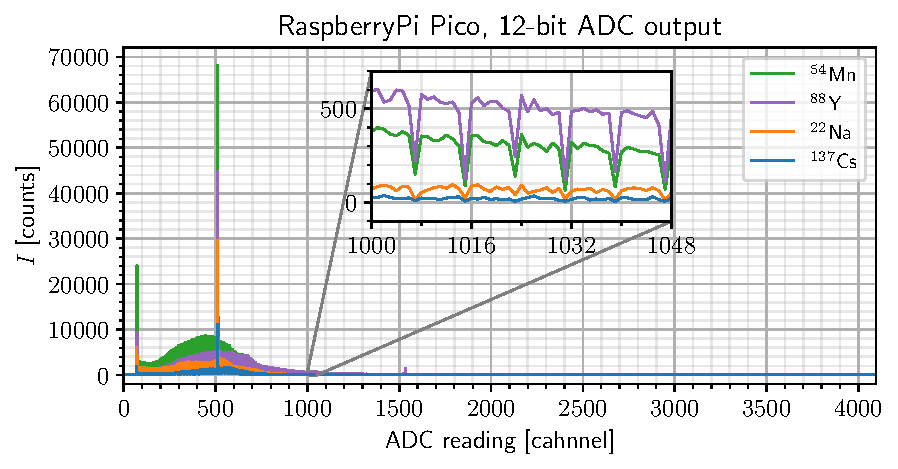
\includegraphics[width=.98\textwidth]{measurements/CW/scaled_raw_adc.pdf}
  \caption{\label{fig:CW_scaled}Histogram of ADC reading per channel, rescaled to 12-bits.}
\end{figure}

\begin{figure}
  \centering
  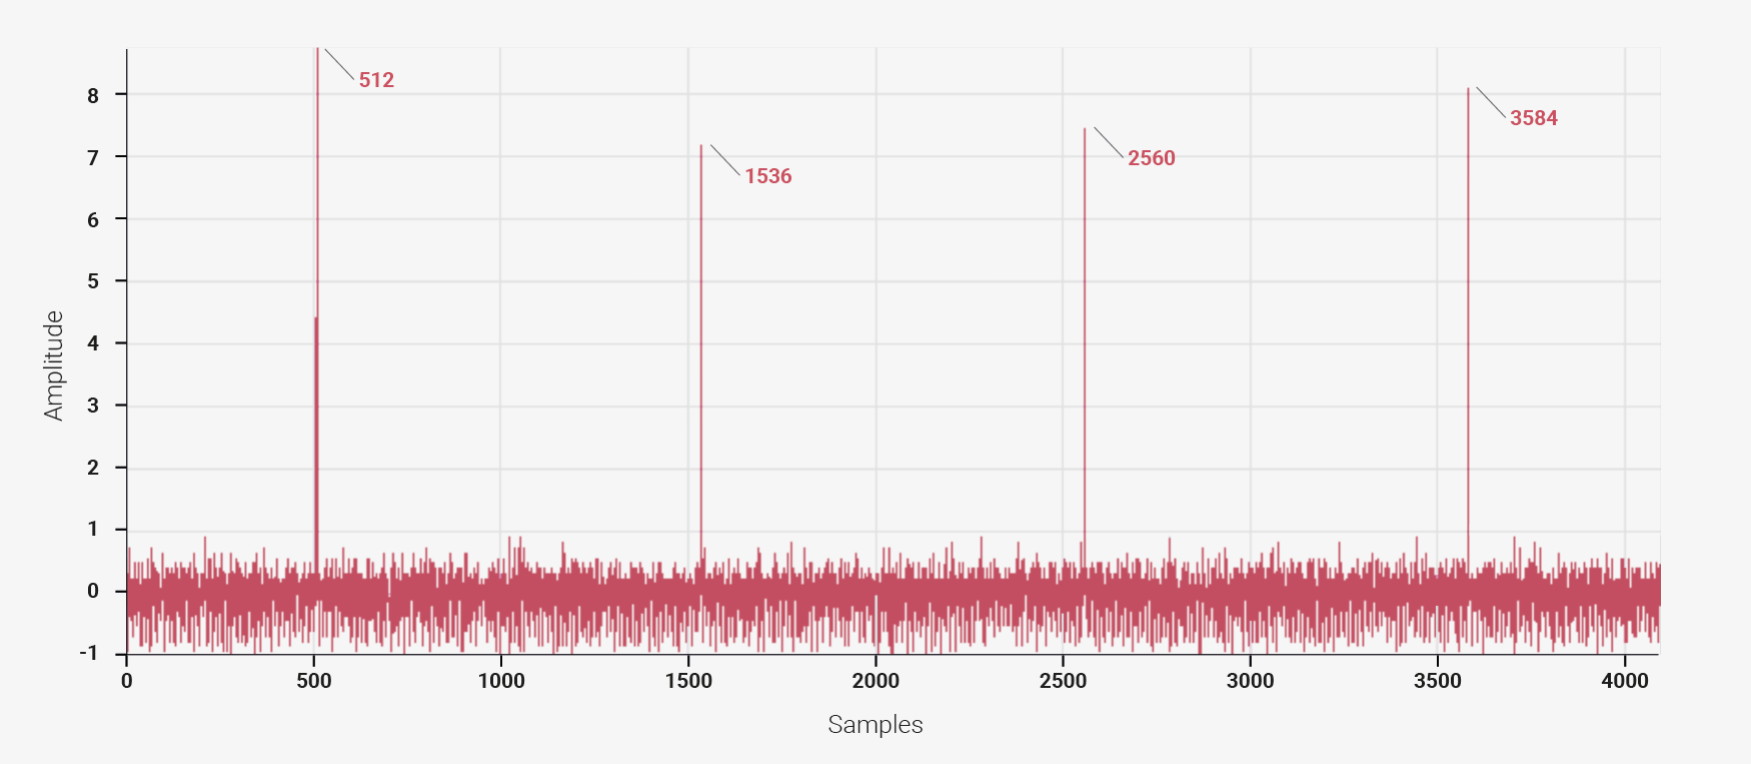
\includegraphics[width=.98\textwidth]{measurements/CW/RP2040_DNL.png}
  \caption{\label{fig:RP2040_DNL}RP2040 ADC Differential Non-Linearity, taken from \cite{datasheet2024rp2040}.}
\end{figure}

The Pico's documentation \cite{datasheet2024RpPico} suggests some changes that can be done to the Pico board that may improve resolution, like reducing the voltage reference (currently set at 3.3V), since this would make the LSB smaller and would take better advantage of our 12-bit resolution.

\subsubsection{Response time}

\begin{figure}[H]
  \centering
  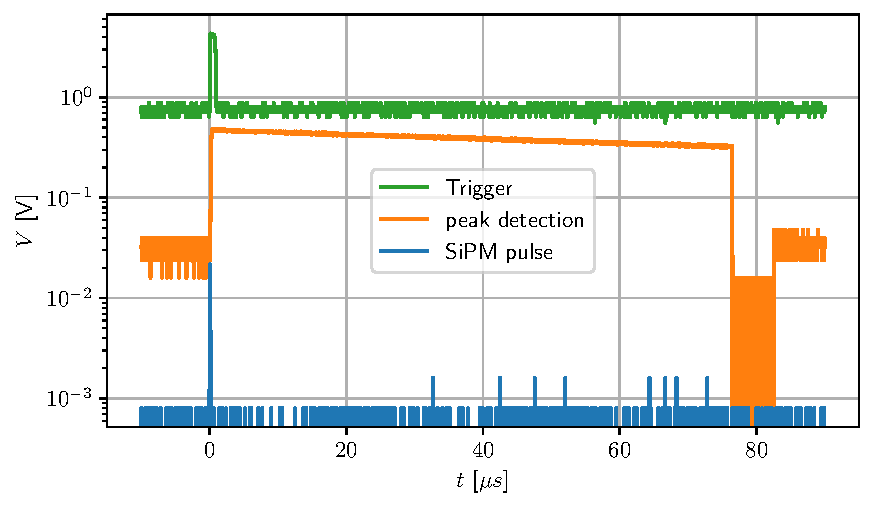
\includegraphics[width=\textwidth]{measurements/CW/Trigger_reset.pdf}
  \caption{\label{fig:measurement_speed}Trigger and measurement time delay after a SiPM pulse.}
\end{figure}

In an attempt to achieve the fastest response possible after a SiPM pulse is sent to the peak detector, an interrupt routine (\texttt{read\_ADC} in \texttt{run.py}) was used to stop all processes and focus on reading the ADC, this is supposed to ensure that the Pico's ADC would read the peak detected signal and the capacitor would be discharged in the shortest time, preventing event loses and pileup with other incoming pulses. 

Figure \ref{fig:measurement_speed} showcases the delay after an incoming SiPM pulse has been detected and processed by the detector, it can be seen that the peak detector's capacitor is discharged by the TriggerReset pin about 76 \unit{\micro\s} after the detector is triggered, this means that the ADC reading could have happened at any moment in that time window. The difference in voltage in the peak detected signal at its maximum and right before the capacitor is discharged is about 176 \unit{\mV}, according to our theoretical LSB, this voltage drop represents a 218 channel difference in the ADC reading.

Increasing the time response could greatly improve the detector's resolution since it would minimize the time delay between incoming pulses and ADC readings, therefore decreasing the error between the recorded value and the real amplitude of the peak-detected signal.

\subsection{Measured spectra}

\begin{figure}[H]
  \centering
  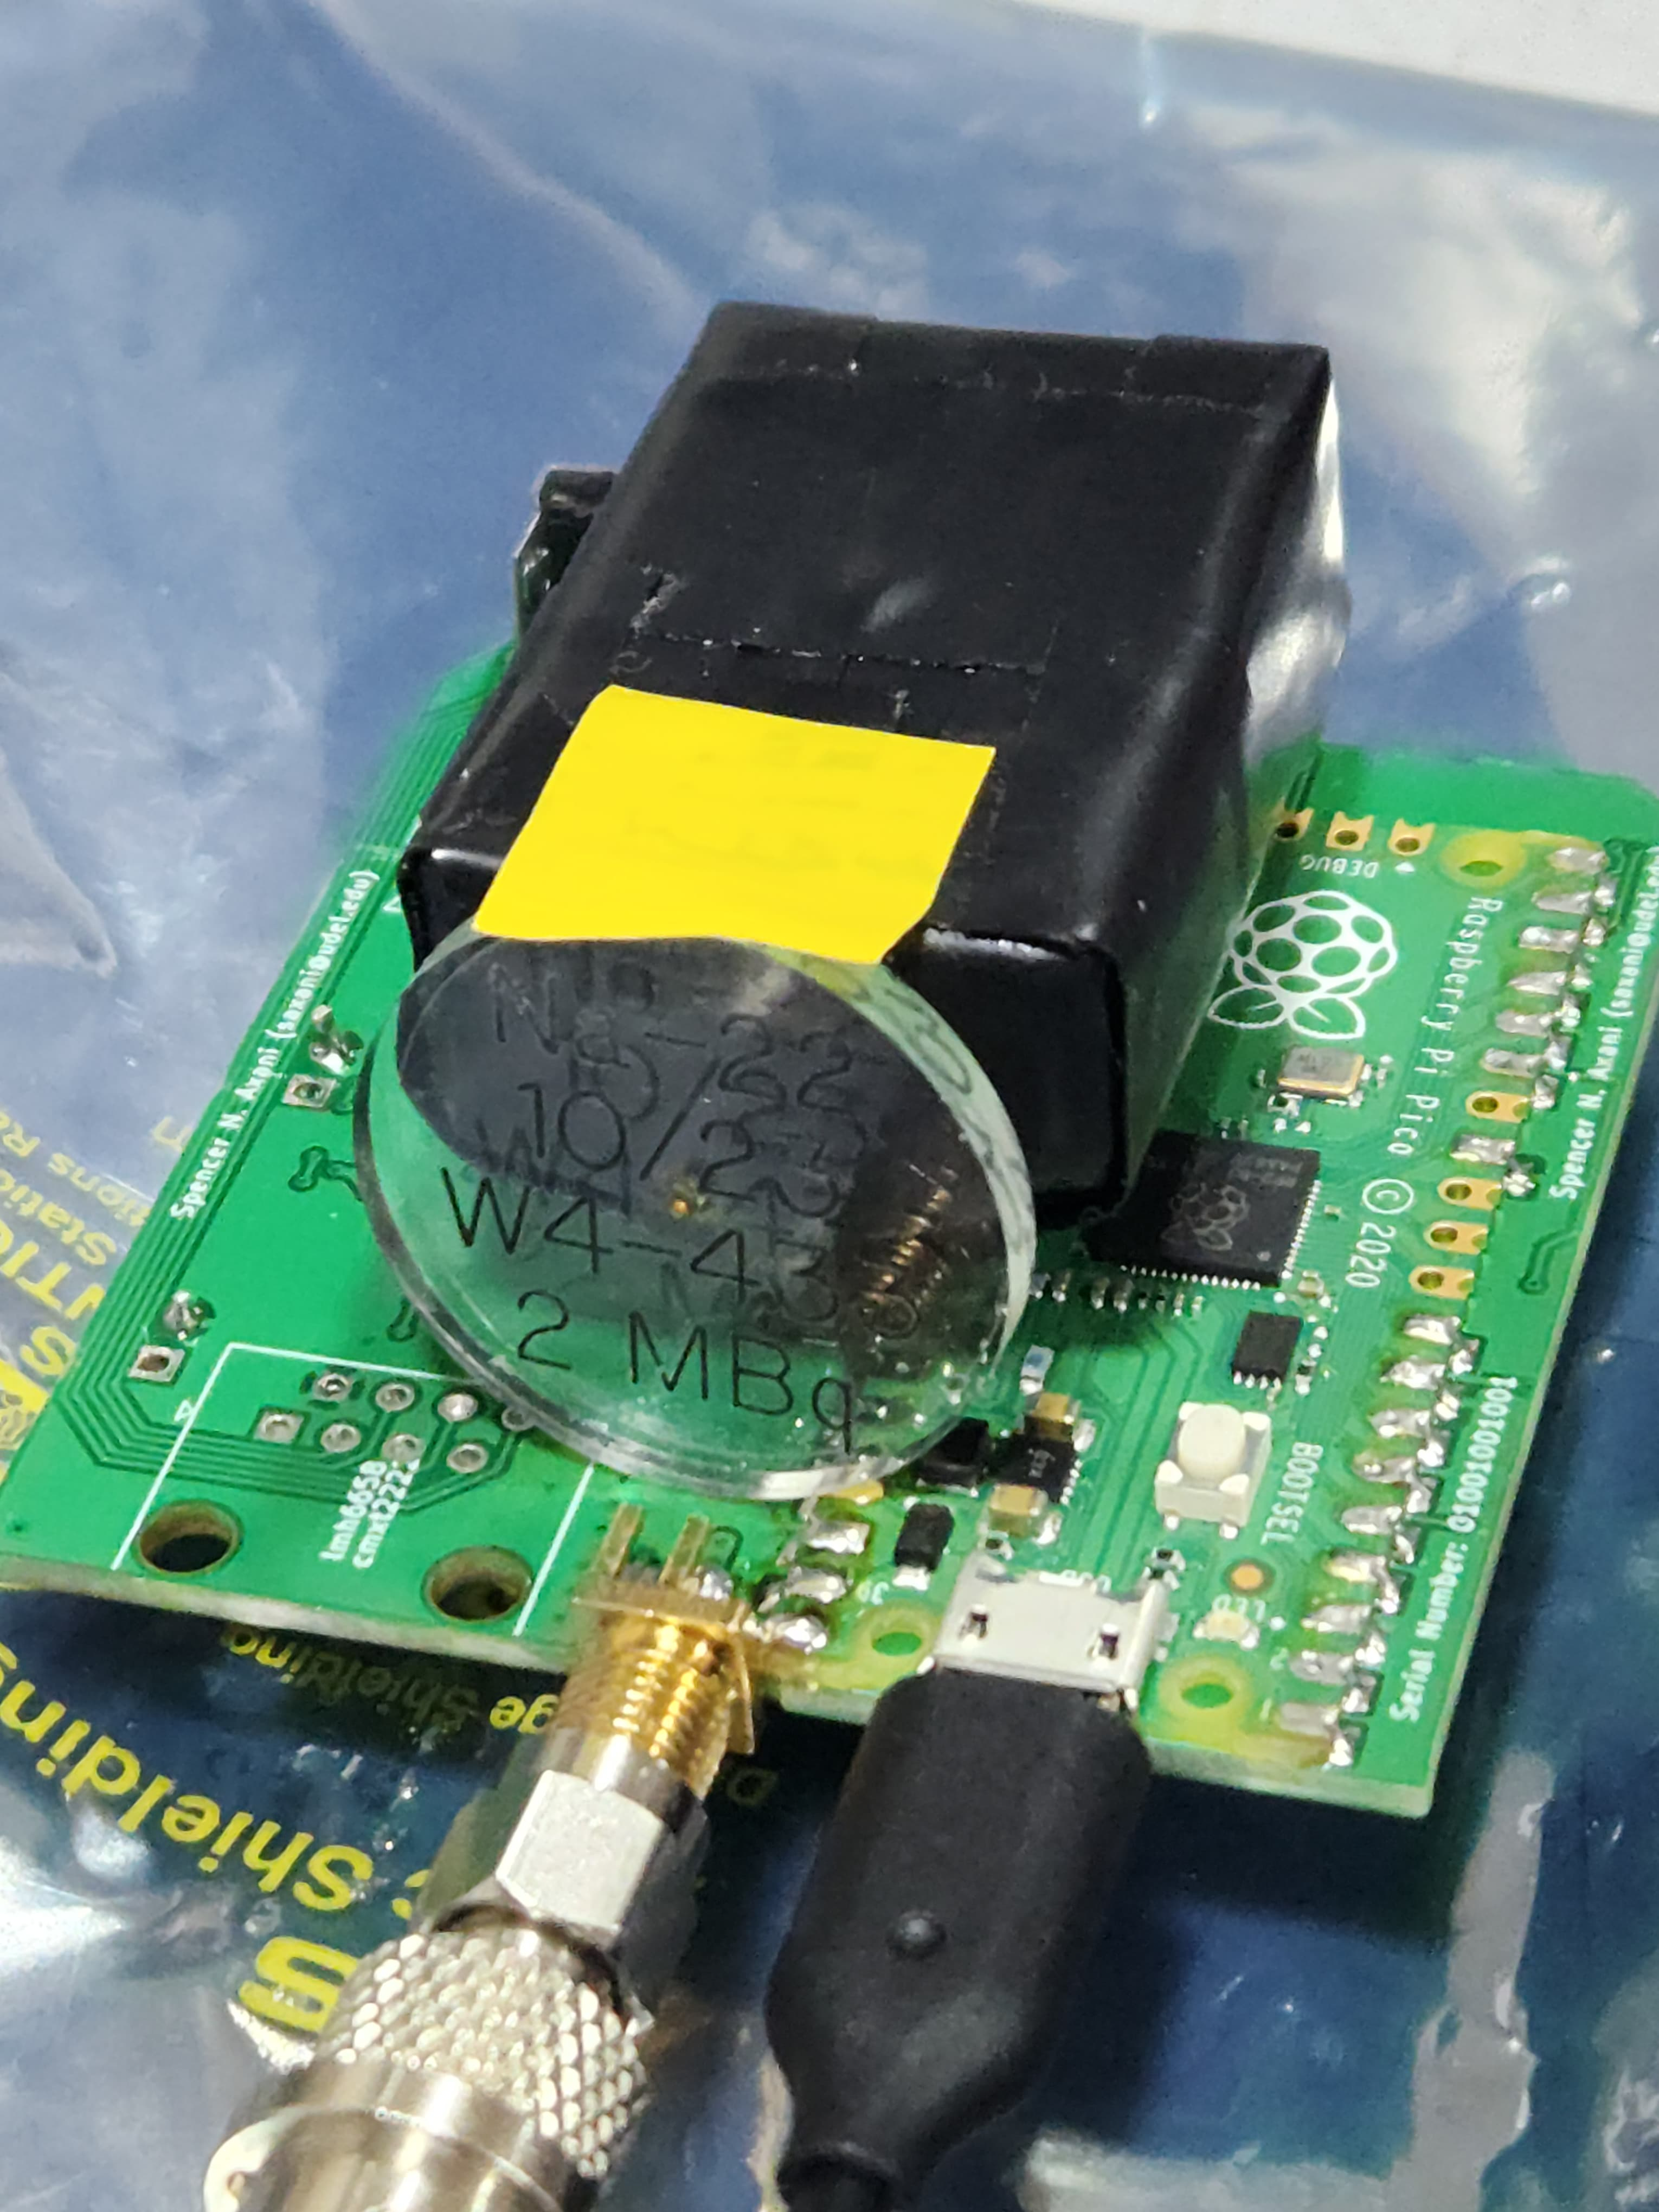
\includegraphics[width=.25\textwidth]{measurements/Source_position.jpg}
  \caption{\label{fig:source_position}Source positioning relative to the detector.}
\end{figure}

Figure \ref{fig:source_position} shows how the radioactive sources were positioned relative to the detector, it is done this way for two reasons: first, it ensures the gamma rays will have a longer travel path inside the crystal, and second, the small distance seems to produce the best results for low activities, such as those of Manganese, Yttrium, and Cesium, on the other hand, the Sodium source was placed 15 \unit{\cm} away from the detector due to its large activity, since moving it closer only increased Compton counts, although a more thorough analysis could be made in order to find an optimum source position.

Figure \ref{fig:CW_spectra} shows the spectra obtained for four different calibrated sources (the same used while testing the CosmicWatch with NIM modules in Sec. \ref{sec:NIM_modules}) while running the \texttt{spectra.py} script on the Pico for one hour. These spectra take into account the ADC shortcomings showcased in Sec. \ref{sec:ADC_shortcomings}, therefore, the channels range from 0 to 4095, the periodically low counts were ``erased'' by grouping the data every 8 channels, and the large DNL in channels 511 and 1536 was removed by taking the average of the previous and next channel. 

Contrary to the spectra shown in sections \ref{sec:RTO6} and \ref{sec:NIM_modules}, in this case, not all of the photopeaks cover enough channels to fit a gaussian to them, this was only possible for Sodium and Cesium, as showcased in Fig. \ref{fig:CW_spectra}. In the case of Manganese and Yttrium, we can only estimate the centroid to lie at the channel with the most counts in their respective photopeaks, which means that it will have an 8-channel error due to the channel-grouping discussed earlier, doing this we get the calibration shown in Fig. \ref{sfig:CW_LYSO_calibration}.

\begin{figure}[H]
  \begin{subfigure}[t]{0.48\textwidth}
    \centering
    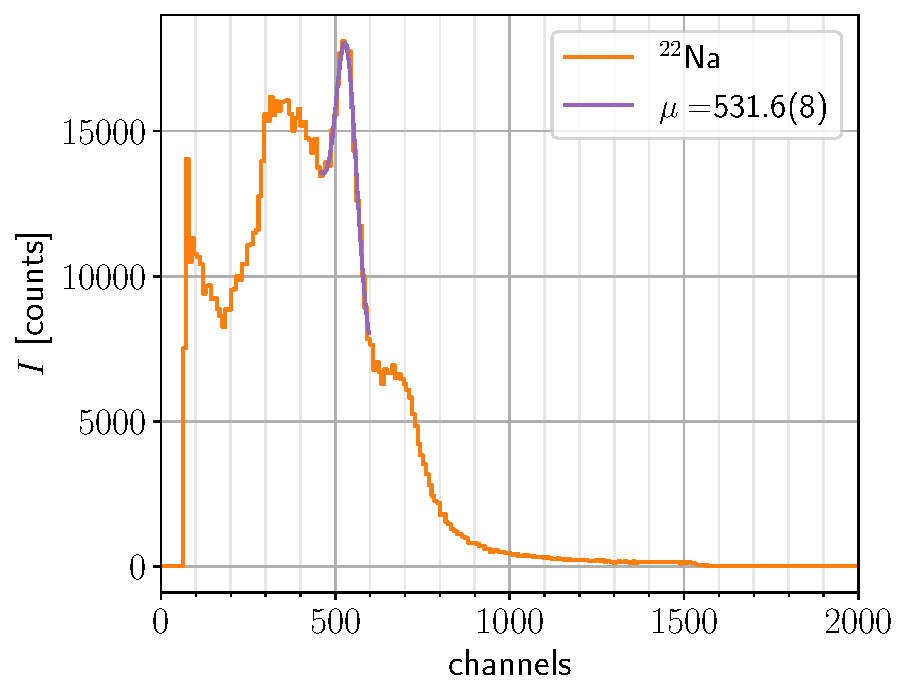
\includegraphics[width=\textwidth]{measurements/CW/22Na.pdf}
    \caption{\label{sfig:CW_22Na}$^{22}$Na, $A=1697.320$ kBq.}
  \end{subfigure}
  \hfill
  \begin{subfigure}[t]{0.48\textwidth}
    \centering
    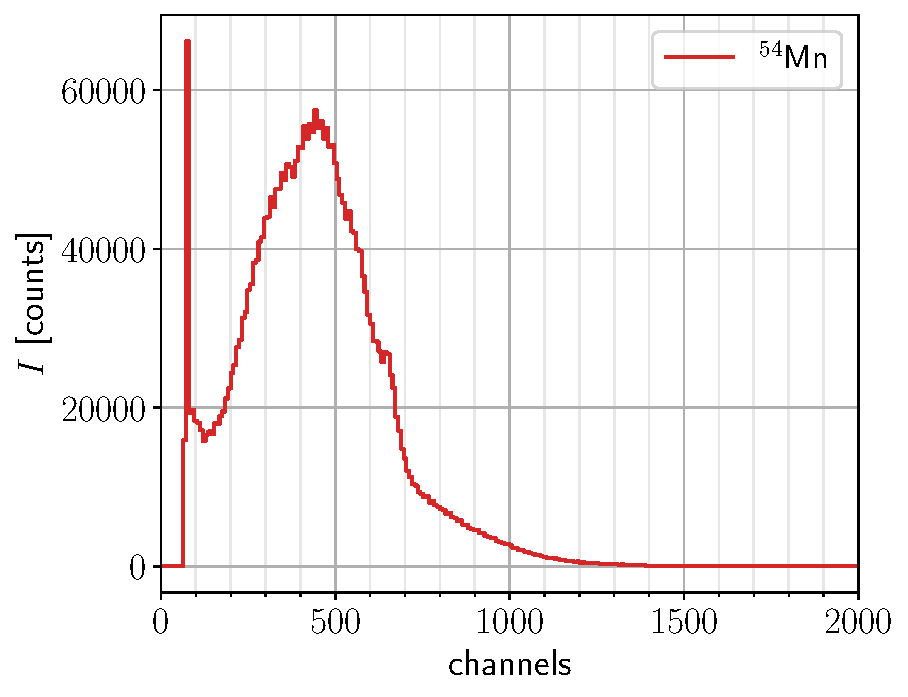
\includegraphics[width=\textwidth]{measurements/CW/54Mn_1.pdf}
    \caption{\label{sfig:C2_54Mn}$^{54}$Mn, $A=623.108$ kBq.}
  \end{subfigure}
  \medskip
  \begin{subfigure}[t]{0.48\textwidth}
    \centering
    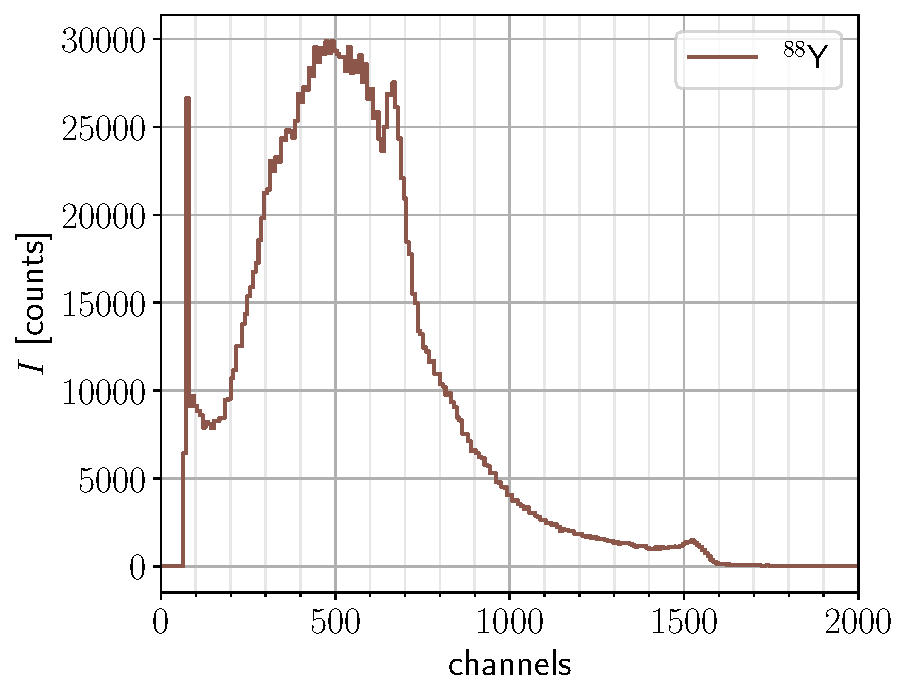
\includegraphics[width=\textwidth]{measurements/CW/88Y_1.pdf}
    \caption{\label{sfig:CW_88Y}$^{88}$Y, $A=251.980$ kBq.}
  \end{subfigure}
  \hfill
  \begin{subfigure}[t]{0.48\textwidth}
    \centering
    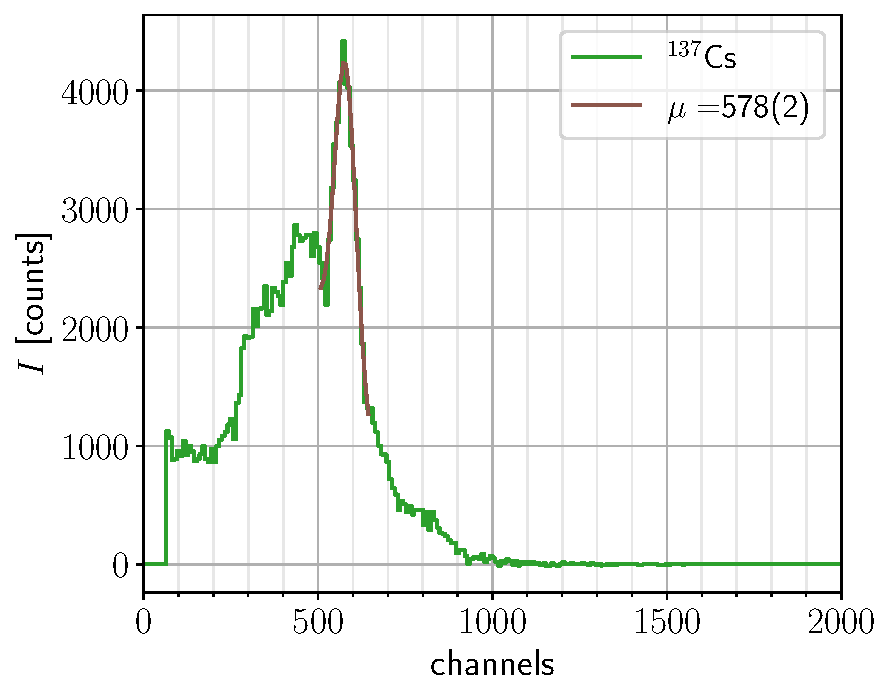
\includegraphics[width=\textwidth]{measurements/CW/137Cs.pdf}
    \caption{\label{sfig:CW_137Cs}$^{137}$Cs, $A=23.139$ kBq.}
  \end{subfigure}
  \caption{\label{fig:CW_spectra}Spectra measured with the Raspberry Pi Pico using the \texttt{spectra.py} script found in Appendix \ref{sec:spectra.py}.}
\end{figure}

As mentioned in subsection \ref{sec:Non-linearity}, the detector's response to variations in SiPM pulse amplitudes is not linear, making necessary the use of an eleven-degree polynomial to represent the peak detector's behavior. Since it was only possible to measure four gamma-ray peaks, it is not possible to use the polynomial calibration showcased in \ref{fig:nonlinearity}, it is for this reason that we have limited our calibration to a linear fit. The lack of a true representation of the detector's nonlinearity is most likely the reason why we find negative energy values in Figure \ref{sfig:CW_joint_spectra}.

Since it was not possible to perform a gaussian fit for all peaks, we can not show an FWHM versus energy comparison which would provide a clear picture of the detector's resolution. Instead, we will have to conform with just the energy resolution at 511 keV, which in this case is 36.5$\%$. Further work needs to be done to increase resolution, some possible alternatives are explored in Chapter \ref{chap:future}.

\begin{figure}[H]
  \begin{subfigure}[t]{\textwidth}
    \centering
    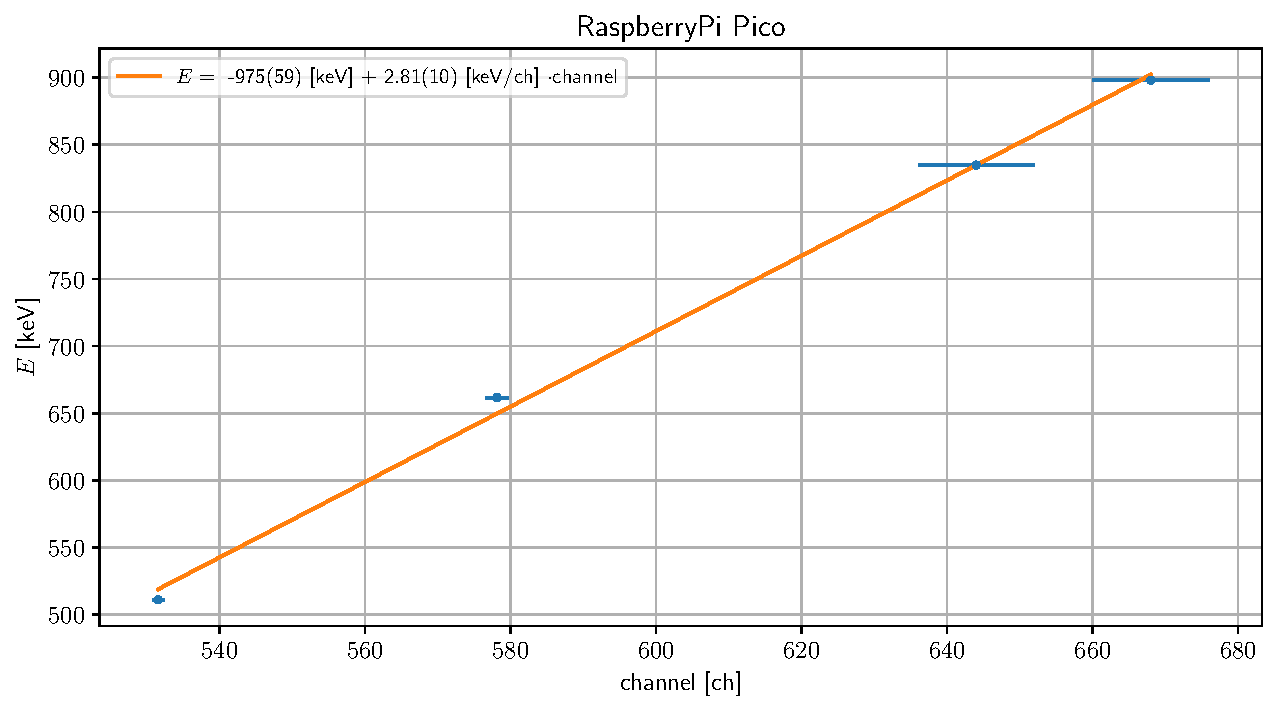
\includegraphics[width=.98\textwidth]{measurements/CW/LYSO_calibration.pdf}
    \caption{\label{sfig:CW_LYSO_calibration}LYSO calibration from Raspberry Pi Pico data. Obtained by fitting gaussian functions to the main peaks of Sodium and Cesium and taking the channel with the most counts in the photopeaks of Manganese and Yttrium.}
  \end{subfigure}
  \medskip
  \begin{subfigure}[t]{\textwidth}
    \centering
    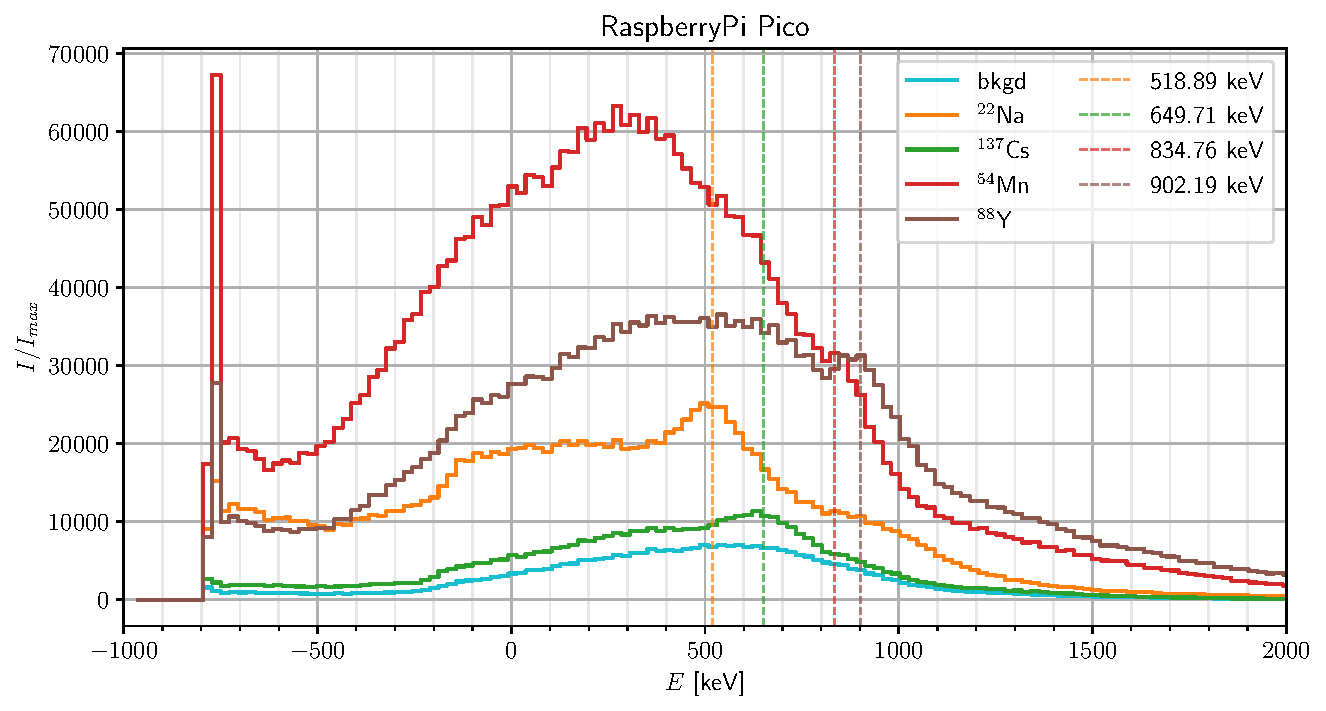
\includegraphics[width=.98\textwidth]{measurements/CW/Calibrated_spectrum.pdf}
    \caption{\label{sfig:CW_joint_spectra}Calibrated spectrum obtained from the channel-energy conversion shown in \subref{sfig:CW_LYSO_calibration}.}
  \end{subfigure}
  \caption{\label{fig:CW_calibration}Gamma-ray spectra obtained with the CosmicWatch detector.}
\end{figure}

\section{Rohde\&Schwarz RTO6 oscilloscope}\label{sec:RTO6}

\begin{figure}[H]
  \begin{subfigure}[t]{0.48\textwidth}
    \centering
    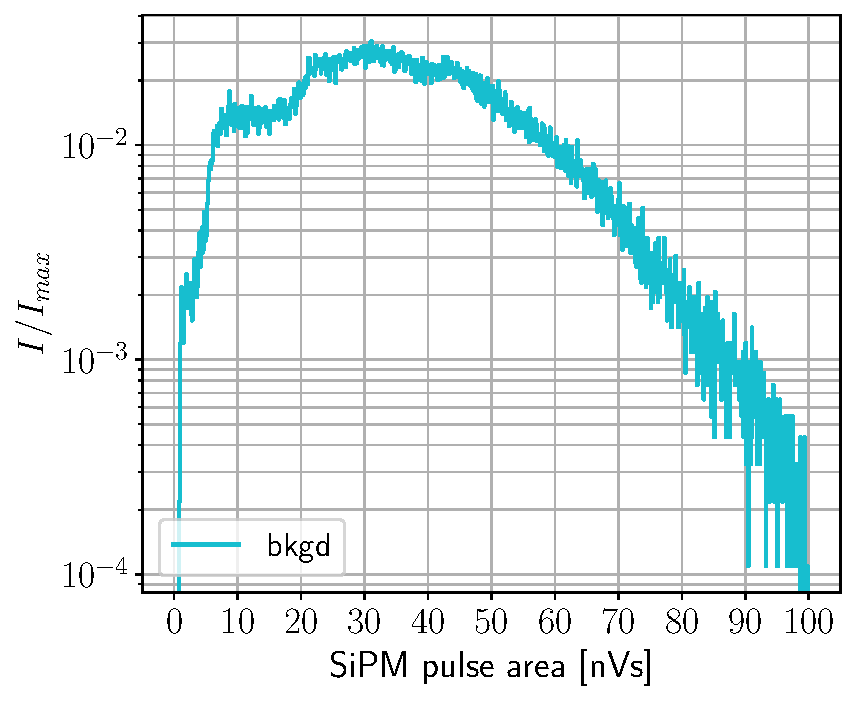
\includegraphics[width=\textwidth]{measurements/RS/teflon-bkgd.pdf}
    \caption{\label{sfig:RS_bkgd}LYSO background.}
  \end{subfigure}
  \hfill
  \begin{subfigure}[t]{0.48\textwidth}
    \centering
    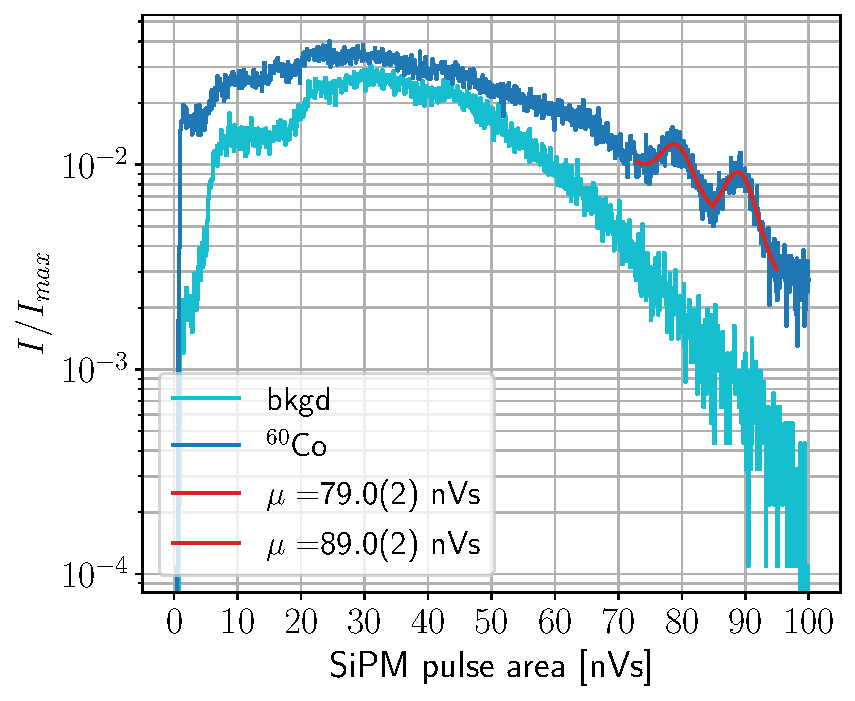
\includegraphics[width=\textwidth]{measurements/RS/teflon-side-Co60.pdf}
    \caption{\label{sfig:RS_60Co}$^{60}$Co.}
  \end{subfigure}
  \medskip
  \begin{subfigure}[t]{0.48\textwidth}
    \centering
    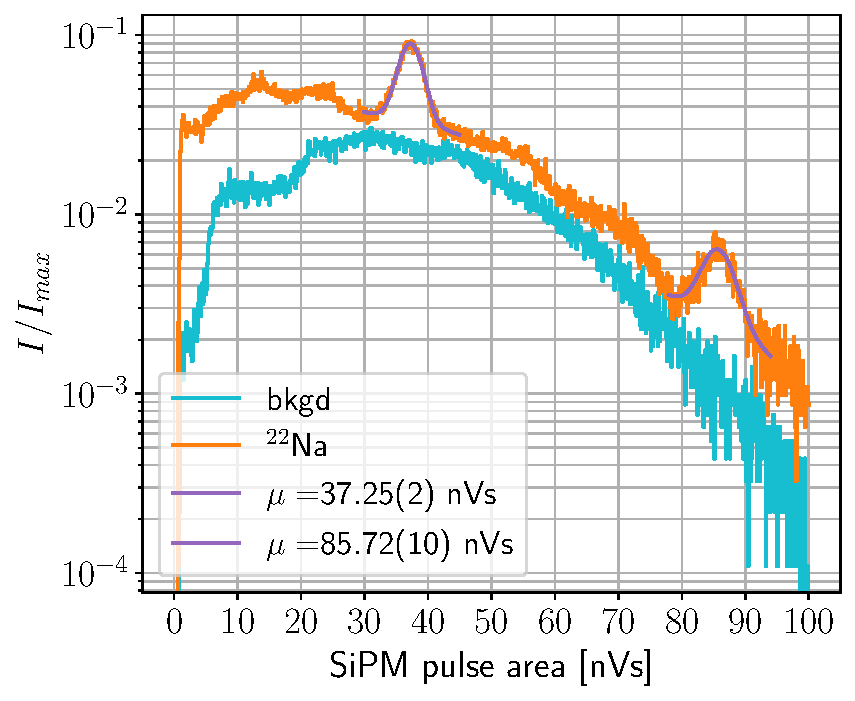
\includegraphics[width=\textwidth]{measurements/RS/teflon-side-Na22.pdf}
    \caption{\label{sfig:RS_22Na}$^{22}$Na.}
  \end{subfigure}
  \hfill
  \begin{subfigure}[t]{0.48\textwidth}
    \centering
    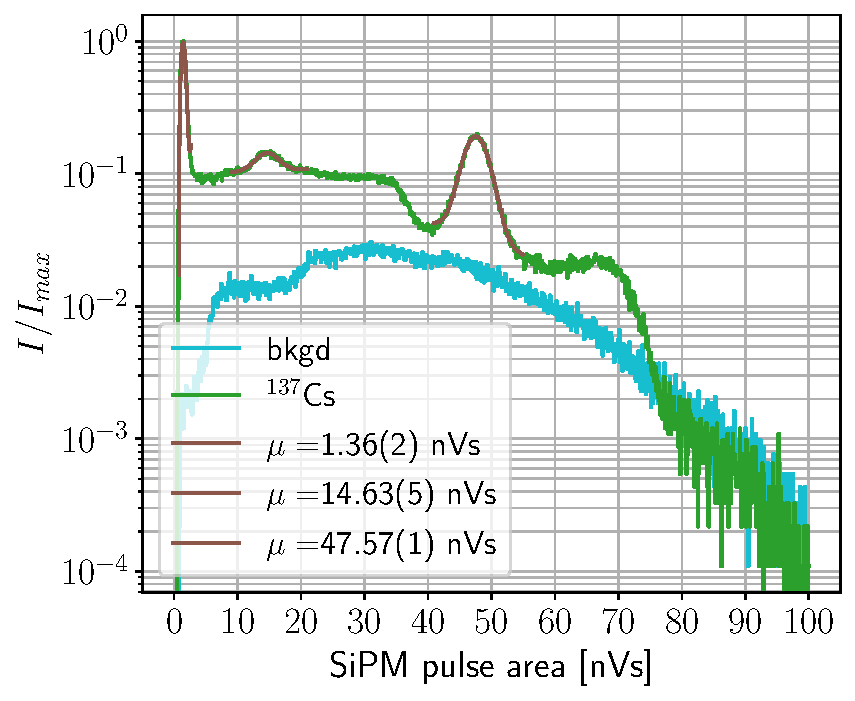
\includegraphics[width=\textwidth]{measurements/RS/teflon-side-Cs137.pdf}
    \caption{\label{sfig:RS_137Cs}$^{137}$Cs.}
  \end{subfigure}
  \caption{\label{fig:RS_spectra}Spectra measured with the histogram functionality of a Rohde\&Schwarz RTO6 oscilloscope. Each graph features the centroid of the Gaussian fitted to each peak.}
\end{figure}

The Rohde\&Schwarz RTO6 oscilloscope was the main troubleshooting tool used to test the detector as a whole. The histogram functionality on the oscilloscope allowed us to also measure spectra from calibrated sources, Figure \ref{fig:RS_spectra} shows the obtained spectra. The $x$ axis measures SiPM pulse areas since the oscilloscope creates histograms based on the area under each SiPM pulse (\textcolor{blue}{blue} signal in Fig. \ref{fig:signal_processing}).

It is important to note here the shape of the background (Fig. \ref{sfig:RS_bkgd}), remembering Figure \ref{fig:LYSO_background}, a sudden increase in intensity should occur at around 290 and 597 \unit{\kilo\eV}, therefore the 511 \unit{\kilo\eV} peak of $^{22}$Na should lie in between these values, while 662 \unit{\kilo\eV} from $^{137}$Cs would lie above the second increase in background counts. These approximations can help us get a notion of what we are seeing in the various spectra illustrated in Fig. \ref{fig:RS_spectra}.

The highest peak in $^{137}$Cs is presumed to be caused by x-ray emissions from lower shell electrons filling the space left by internal conversion electrons, this peak is also featured in Figure \ref{fig:Cs137_description}. One important feature in the cesium spectrum is the relatively high intensities passed the photopeak (at 47.57(1) nVs according to the gaussian fit), this is not due to LYSO background since these counts greatly exceed the expected background.

Fitting gaussian functions to the main peaks one can get the relation between energy and pulse area (Fig. \ref{sfig:RS_LYSO_calibration_low_peaks}) based on the decay schemes shown in Figure \ref{fig:decay_schemes}. Considering the x-ray and backscattering peaks of $^{137}$Cs, however, seems to cause an overestimation of the energies, as can be seen in Figure \ref{sfig:RS_LYSO_calibrated_spectrum_low_peaks}, where the pair-production peak of sodium, for example, lies at 535.95 keV instead of 511 keV. The calibration shown in Figure \ref{sfig:RS_LYSO_calibration} does not take into account the troublesome peaks of Cesium, better estimating high energy peaks, this however results in negative-energy predictions at the lower energy range in the spectrum.

\begin{figure}[H]
  \begin{subfigure}[t]{\textwidth}
    \centering
    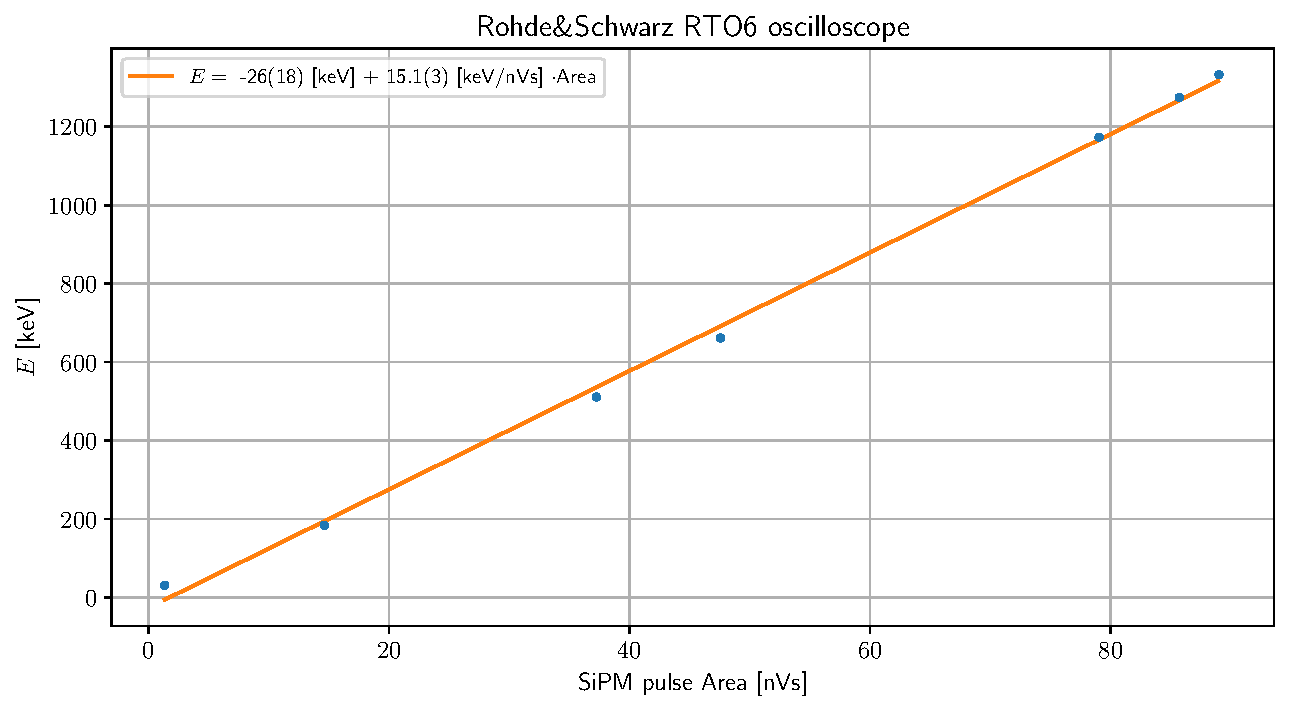
\includegraphics[width=.98\textwidth]{measurements/RS/LYSO_calibration_low_peaks.pdf}
    \caption{\label{sfig:RS_LYSO_calibration_low_peaks}LYSO calibration from Rohde\&Schwarz oscilloscope data. Obtained by fitting gaussian functions to the main peaks shown in Fig \ref{sfig:RS_60Co}, \subref{sfig:RS_22Na}, and \subref{sfig:RS_137Cs}.}
  \end{subfigure}
  \medskip
  \begin{subfigure}[t]{\textwidth}
    \centering
    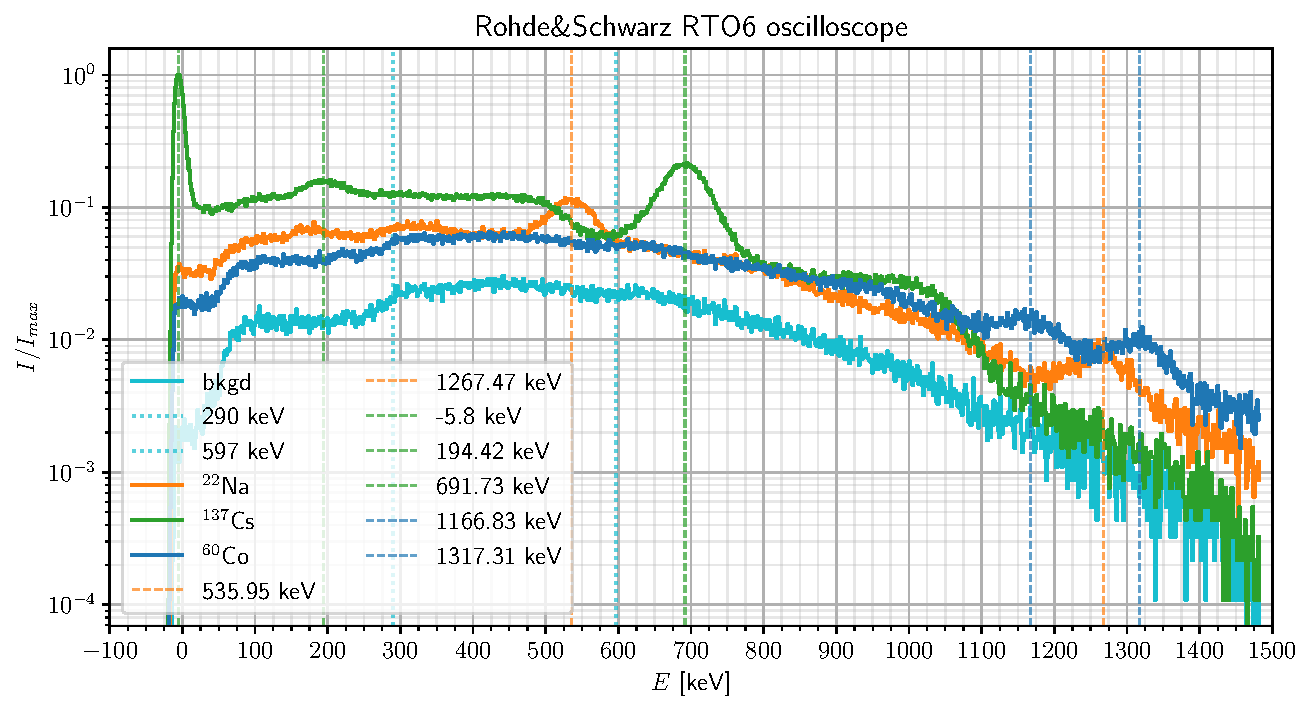
\includegraphics[width=.98\textwidth]{measurements/RS/Calibrated_spectrum_low_peaks.pdf}
    \caption{\label{sfig:RS_LYSO_calibrated_spectrum_low_peaks}Calibrated spectrum obtained from the channel-energy conversion shown in \subref{sfig:RS_LYSO_calibration_low_peaks}.}
  \end{subfigure}
  \caption{\label{fig:RS_low_peaks_calibration}Calibrated spectrum taking into account the x-ray and backscattering peaks of $^{137}$Cs.}
\end{figure}

\begin{figure}[H]
  \begin{subfigure}[t]{\textwidth}
    \centering
    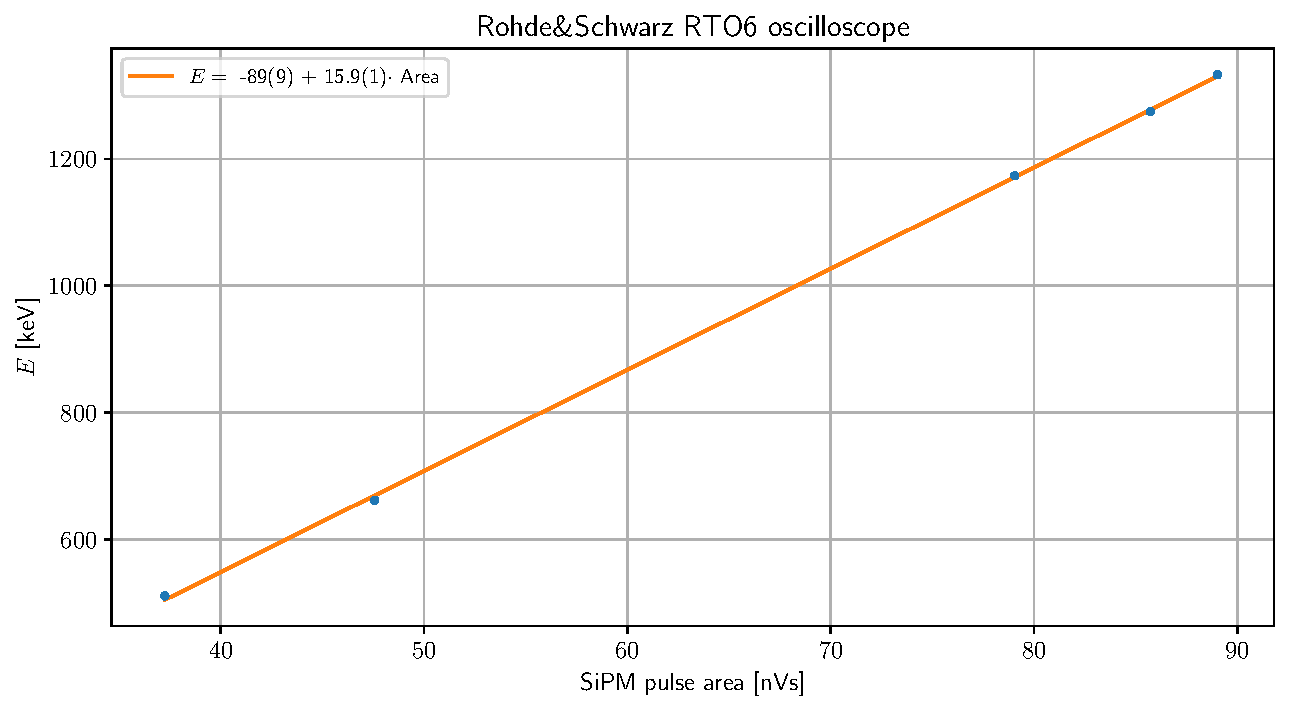
\includegraphics[width=.98\textwidth]{measurements/RS/LYSO_calibration.pdf}
    \caption{\label{sfig:RS_LYSO_calibration}LYSO calibration from Rohde\&Schwarz oscilloscope data. Excluding x-ray and backscattering peaks from \subref{sfig:RS_137Cs}.}
  \end{subfigure}
  \medskip
  \begin{subfigure}[t]{\textwidth}
    \centering
    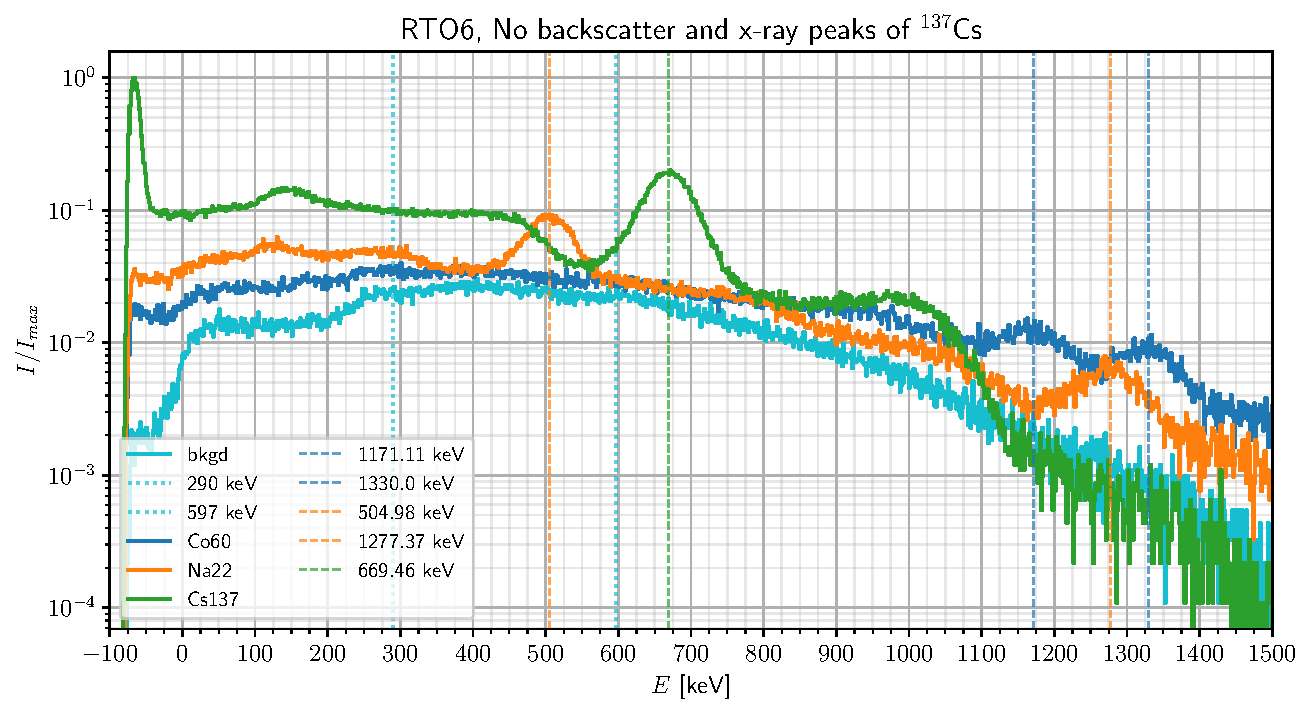
\includegraphics[width=.98\textwidth]{measurements/RS/Calibrated_spectrum.pdf}
    \caption{\label{sfig:RS_LYSO_calibrated_spectrum}Calibrated spectrum obtained from the channel-energy conversion shown in \subref{sfig:RS_LYSO_calibration}.}
  \end{subfigure}
  \caption{\label{fig:RS_calibration}Calibrated spectrum, ignoring the x-ray and backscattering peaks of $^{137}$Cs.}
\end{figure}

\newpage
In general, the $\chi^2$ results for the multiple fits performed were much better while ignoring the low energies of Cesium, leading us to conclude that this might be optimal, obtaining the final FWHM vs Energy calibration shown in Fig. \ref{fig:RS_FWHM}. This results in an energy resolution of 13.5\% at 511 keV.

\begin{figure}[H]
  \centering
  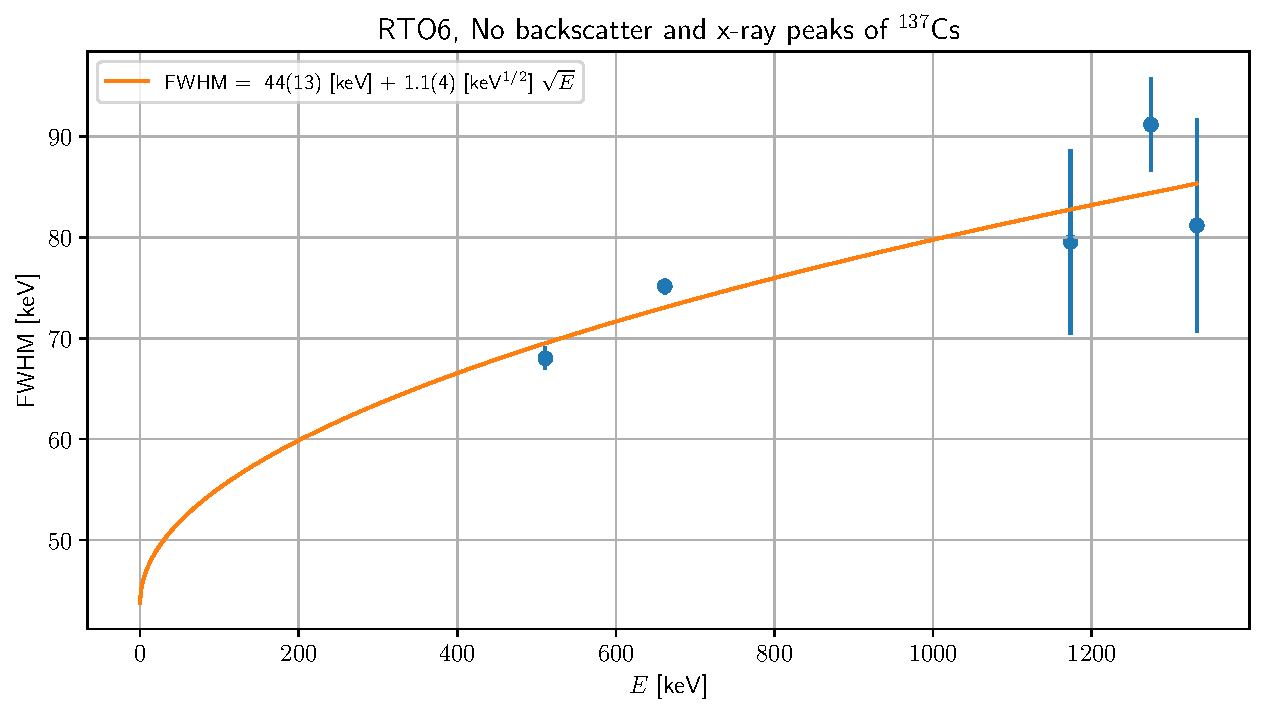
\includegraphics[width=.98\textwidth]{measurements/RS/FWHM.pdf}
  \caption{\label{fig:RS_FWHM}FWHM as a function of energy from spectra obtained with a Rohde\&Schwarz RTO6 oscilloscope.}
\end{figure}

\newpage
\section{NIM modules}\label{sec:NIM_modules}

In the same way the CosmicWatch was studied with the Rohde\&Schwarz oscilloscope, NIM modules were used to get a LYSO calibration when coupled to the SiPM, this section shows some of the results obtained.

\subsection{Odd features}

While testing the detector response some odd features were found in the measured spectra, they are yet to be understood and present an interesting study case, Figure \ref{fig:NIM_odd_features} showcases some of the spectra obtained that illustrate these anomalies.

$^{54}$Mn, is a monoenergetic source, meaning that it only produces one gamma ray, in this case at 835 \unit{\kilo\eV}, which lies slightly above 662 \unit{\kilo\eV} ($^{137}$Cs), therefore, the peak in channel 259 in Fig. \ref{sfig:NIM_odd_54Mn} should correspond to the gamma emission from Manganese. However, there is again a very high number of events above the photopeak, which is not expected, since 835 \unit{\kilo\eV} is the maximum energy one should see in this spectrum. Aside from this, it is also clear that the shape of this peak does not fully adjust to a gaussian distribution, showing that there is an underlying structure that has not been explained. These odd features can also be seen in $^{137}$Cs.

\begin{figure}[H]
  \centering
  \begin{subfigure}[t]{0.53\textwidth}
    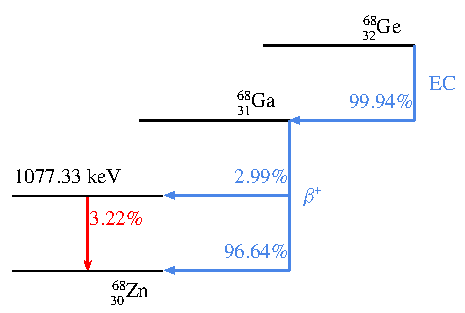
\includegraphics[width=\textwidth]{measurements/68Ge-decay.pdf}
    \caption{\label{sfig:68Ge_decay_scheme}}
  \end{subfigure}
  \begin{subfigure}[t]{0.425\textwidth}
    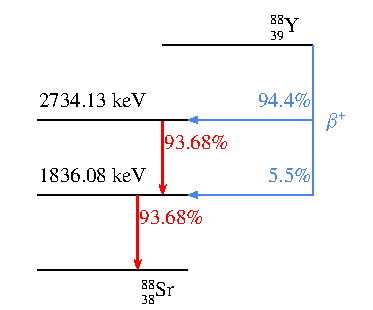
\includegraphics[width=\textwidth]{measurements/88Y-decay.pdf}
    \caption{\label{sfig:88Y_decay_scheme}}
  \end{subfigure}
  \caption{\label{fig:some_decay_schemes}Decay schemes for $^{68}$Ge and $^{88}$Y}
\end{figure}

In principle, $^{68}$Ge should have a spectrum very similar to $^{22}$Na, in this case, however, the decay chain most often ends in a stable state of $^{68}$Zn as illustrated in Fig. \ref{sfig:68Ge_decay_scheme}, this means that the only appreciable peak should lie at 511 \unit{\kilo\eV}, due to pair production from the 1077.33 \unit{\kilo\eV} gamma emission and the subsequent positron annihilation. This agrees with Fig. \ref{sfig:NIM_odd_68Ge}, notably, however, there are very few counts at energies above 511 \unit{\kilo\eV}, which is not the case for the other sources, they present high counts above their respective photopeak. This may be due to the low activity of the source. 

\begin{figure}[H]
  \begin{subfigure}[t]{0.47\textwidth}
    \centering
    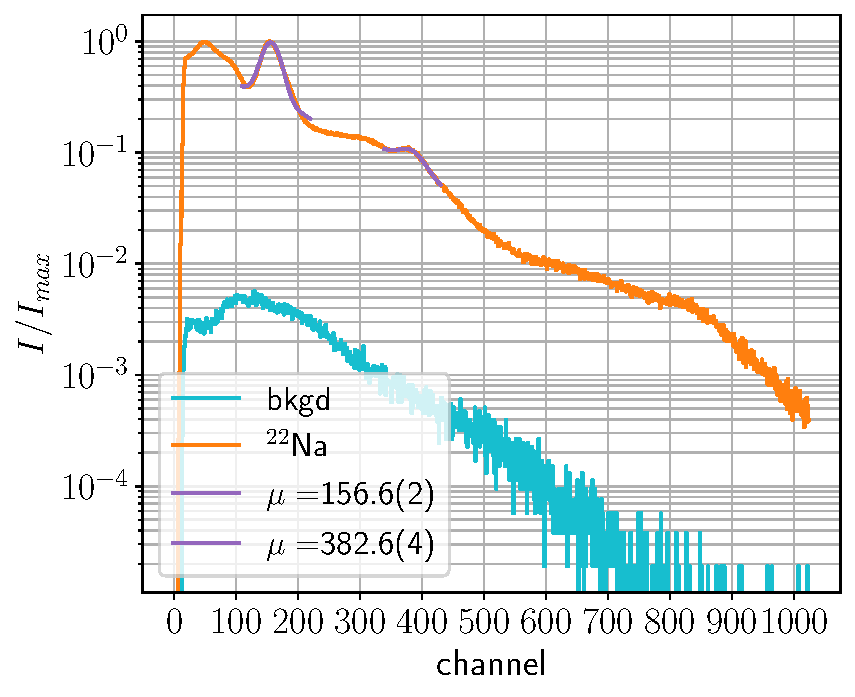
\includegraphics[width=\textwidth]{measurements/NIM/odd_features/22Na.pdf}
    \caption{\label{sfig:NIM_odd_22Na}$^{22}$Na, $A=1697.320$ kBq.}
  \end{subfigure}
  \hfill
  \begin{subfigure}[t]{0.47\textwidth}
    \centering
    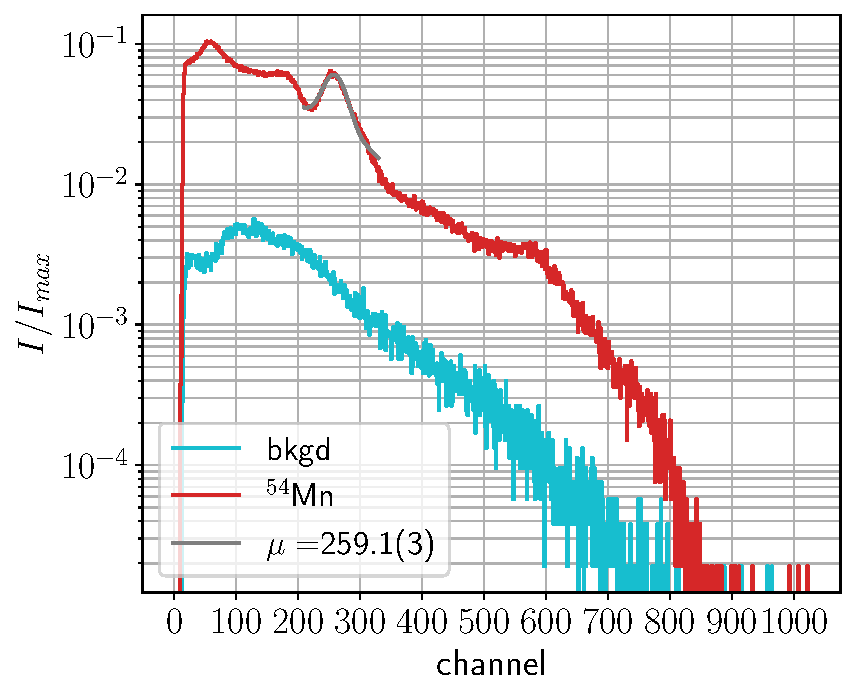
\includegraphics[width=\textwidth]{measurements/NIM/odd_features/54Mn.pdf}
    \caption{\label{sfig:NIM_odd_54Mn}$^{54}$Mn, $A=623.108$ kBq.}
  \end{subfigure}
  \medskip
  \begin{subfigure}[t]{0.47\textwidth}
    \centering
    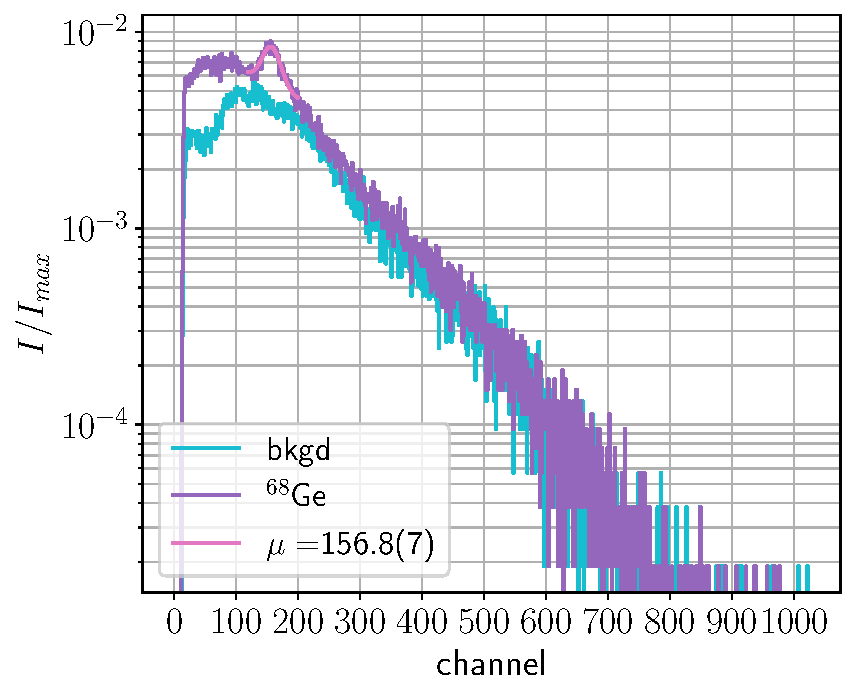
\includegraphics[width=\textwidth]{measurements/NIM/odd_features/68Ge.pdf}
    \caption{\label{sfig:NIM_odd_68Ge}$^{68}$Ge, $A=$? kBq.}
  \end{subfigure}
  \hfill
  \begin{subfigure}[t]{0.47\textwidth}
    \centering
    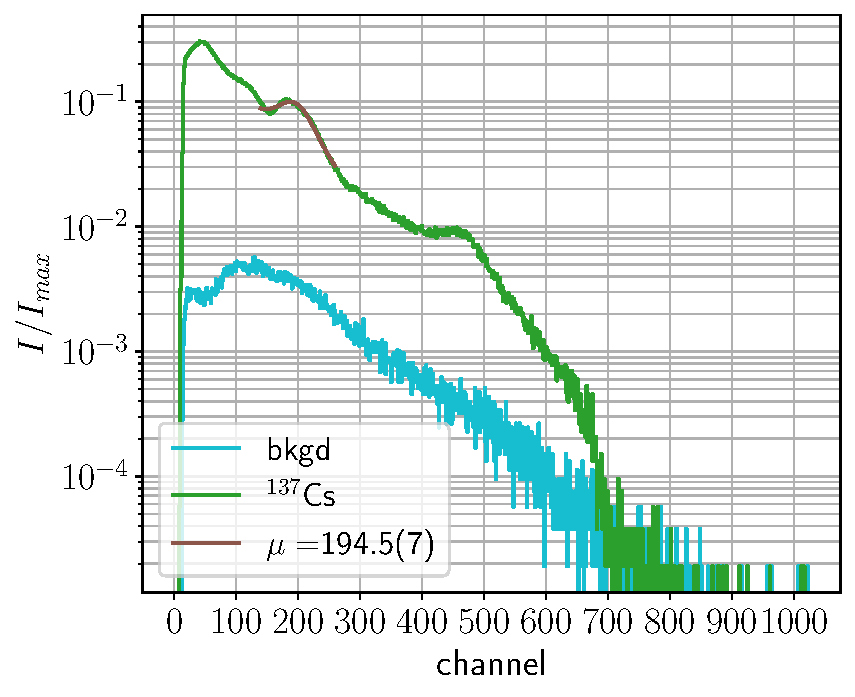
\includegraphics[width=\textwidth]{measurements/NIM/odd_features/137Cs_HA.pdf}
    \caption{\label{sfig:NIM_odd_137Cs}$^{137}$Cs, $A=30790.372$ kBq.}
  \end{subfigure}
  \caption{\label{fig:NIM_odd_features}Spectra measured with a Timing Filter Amplifier and Analog to Digital Converter NIM modules. Each graph features the isotope used, its activity at the time of measurement, and the centroid of the Gaussian fitted to each peak. The $x$ axis gives channels since the ADC creates a histogram based on pulse area. Some odd features can be seen in these spectra, like the large number of counts above the Cesium and Manganese photopeaks.}
\end{figure}

The Cesium spectrum shown in Fig. \ref{sfig:NIM_odd_137Cs} was taken while placing the source 10 cm away from the detector, trying to reduce the count rate due to the large activity of the source, nonetheless, this resulted in an oddly shaped photopeak, and therefore a comparatively large FWHM

%\begin{figure}[H]
%  \centering
%  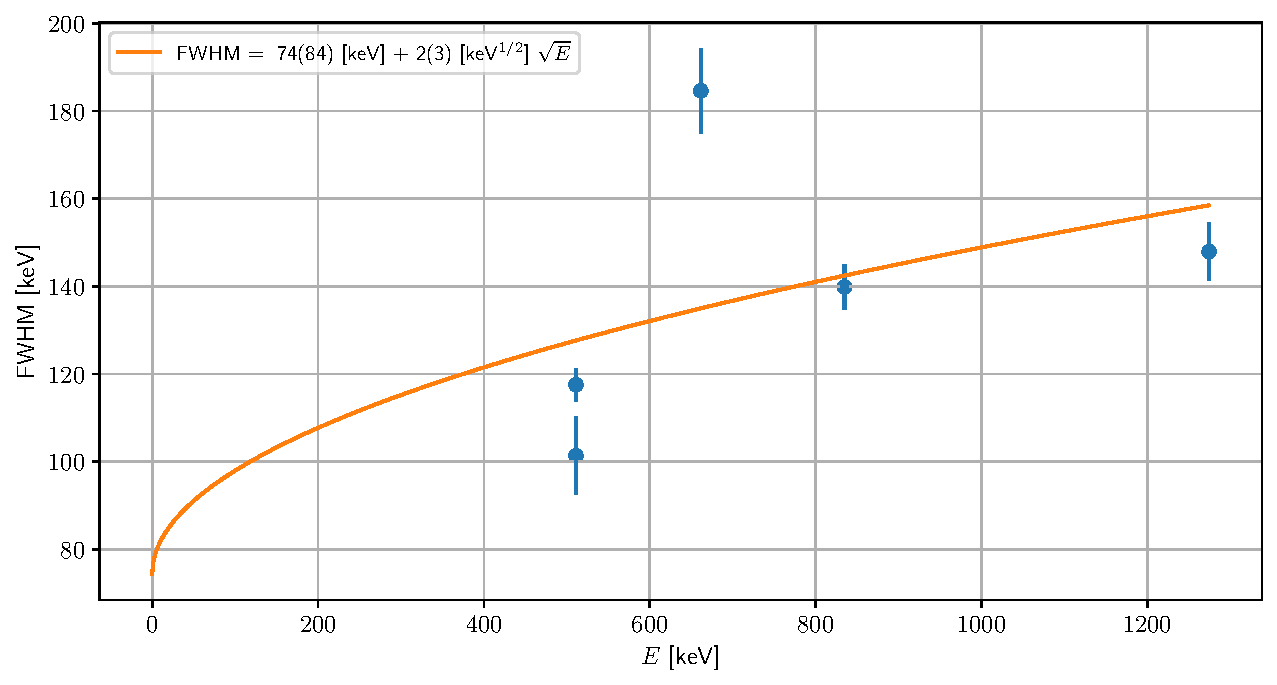
\includegraphics[width=.98\textwidth]{measurements/NIM/odd_features/FWHM.pdf}
%  \caption{\label{fig:NIM_odd_FWHM}FWHM obtained from gaussian fits to the photo- and positron-annihilation peaks shown in \ref{fig:NIM_odd_features}.}
%\end{figure}

\subsection{Calibration}

Following the goal of this work, multiple spectra were measured trying to find the NIM-modules setup that would optimize energy resolution. As expressed in \cite[sec.~4.4.3]{gilmore2008practical}: ``theory suggests that the lowest noise contribution is found when the integration and differentiation times are made equal. On all modern amplifiers, the shaping time constants are made equal and are controlled by a single selector knob.'' In our case, however, the integration and differentiation times were controlled independently, since we used a Canberra Model 2111 Timing Filter Amplifier \cite{CanberraTFA}. So far, the best results were found while using the OUT setup for both time constants, corresponding to 4 ns of integration time and 160 $\mu$s of differentiation time. 

Even though the FWHM does not vary significantly for different time-constant setups, the OUT configuration produced the most accurate calibrations achieved, obtaining an energy resolution of 25.2\% at 511 keV. Further work needs to be done to better understand the origin of the odd features presented above, this may greatly influence the energy resolution since, as can be seen in the Manganese spectrum, not all the peaks present a truly gaussian form.

\begin{figure}[H]
  \centering
  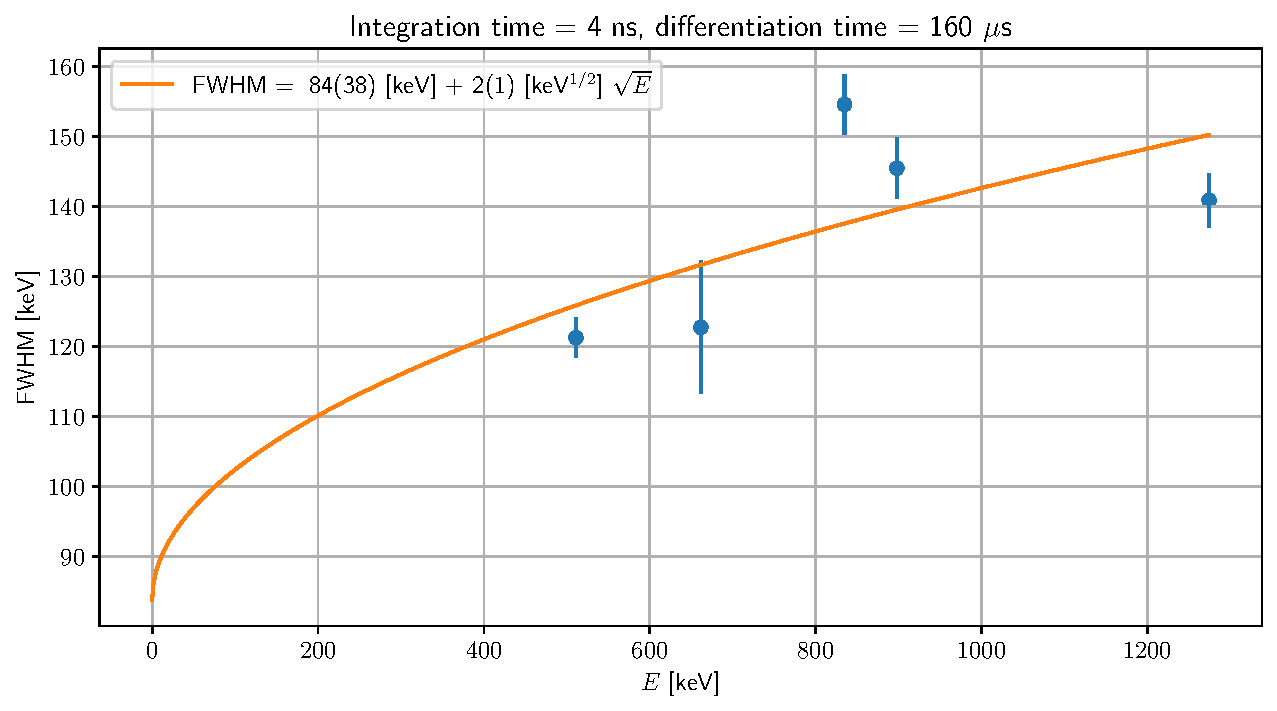
\includegraphics[width=.98\textwidth]{measurements/NIM/2024-05-24/outD/FWHM.pdf}
  \caption{\label{fig:NIM_FWHM}FWHM obtained from gaussian fits to the photo- and positron-annihilation peaks shown in \ref{fig:NIM_spectra}.}
\end{figure}

It is worth noting the great similarities between Figures \ref{sfig:NIM_54Mn}-\subref{sfig:NIM_88Y} and the features explained in subsection \ref{sec:gammas_in_the_detector}, each showcasing a clear photopeak, Compton edge, and backscattering peak.

\begin{figure}[H]
  \begin{subfigure}[t]{0.47\textwidth}
    \centering
    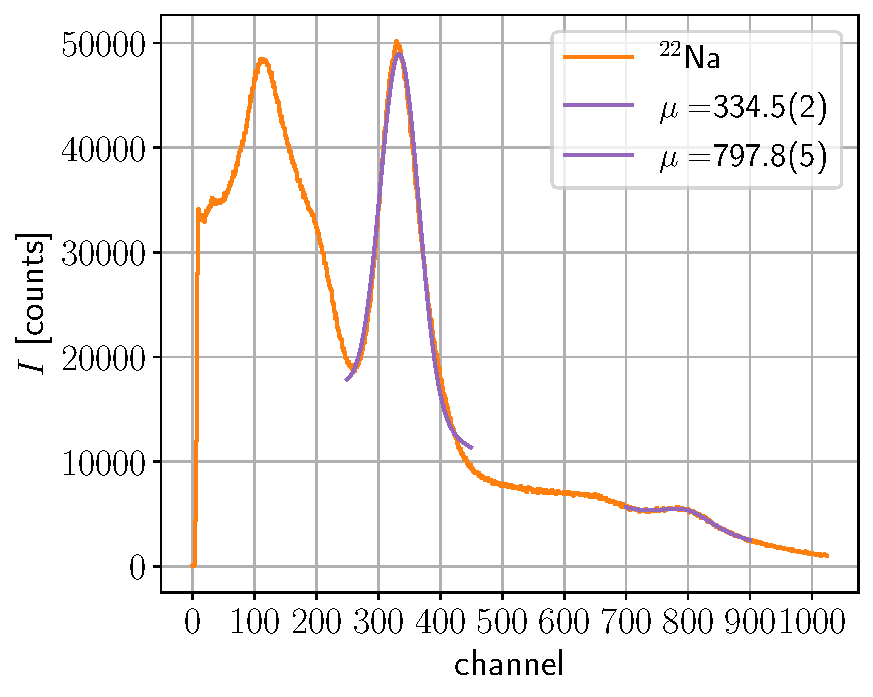
\includegraphics[width=\textwidth]{measurements/NIM/2024-05-24/outD/outD_22Na.pdf}
    \caption{\label{sfig:NIM_22Na}$^{22}$Na, $A=1697.320$ kBq.}
  \end{subfigure}
  \hfill
  \begin{subfigure}[t]{0.47\textwidth}
    \centering
    \includegraphics[width=\textwidth]{measurements/NIM/2024-05-24/outD/outD_54Mn.pdf}
    \caption{\label{sfig:NIM_54Mn}$^{54}$Mn, $A=623.108$ kBq.}
  \end{subfigure}
  \medskip
  \begin{subfigure}[t]{0.47\textwidth}
    \centering
    \includegraphics[width=\textwidth]{measurements/NIM/2024-05-24/outD/outD_88Y.pdf}
    \caption{\label{sfig:NIM_88Y}$^{88}$Y, $A=251.980$ kBq.}
  \end{subfigure}
  \hfill
  \begin{subfigure}[t]{0.47\textwidth}
    \centering
    \includegraphics[width=\textwidth]{measurements/NIM/2024-05-24/outD/outD_137Cs.pdf}
    \caption{\label{sfig:NIM_137Cs}$^{137}$Cs, $A=23.139$ kBq.}
  \end{subfigure}
  \caption{\label{fig:NIM_spectra}Spectra measured with a Timing Filter Amplifier and Analog to Digital Converter NIM modules. The $x$ axis measures channels since the ADC creates a histogram based on pulse area. Each graph features the centroid of the Gaussian fitted to each peak.}
\end{figure}

\begin{figure}[H]
  \begin{subfigure}[t]{\textwidth}
    \centering
    \includegraphics[width=.98\textwidth]{measurements/NIM/2024-05-24/outD/LYSO_calibration.pdf}
    \caption{\label{sfig:NIM_LYSO_calibration}LYSO calibration from NIM modules data. Obtained by fitting gaussian functions to the main peaks shown in Fig \ref{sfig:NIM_22Na} to \subref{sfig:NIM_137Cs}.}
  \end{subfigure}
  \medskip
  \begin{subfigure}[t]{\textwidth}
    \centering
    \includegraphics[width=.98\textwidth]{measurements/NIM/2024-05-24/outD/Calibrated_spectrum.pdf}
    \caption{\label{sfig:NIM_LYSO_calibrated_spectrum}Calibrated spectrum obtained from the channel-energy conversion shown in \subref{sfig:NIM_LYSO_calibration}.}
  \end{subfigure}
  \caption{\label{fig:NIM_calibration}Gamma-ray spectra obtained with NIM modules.}
\end{figure}

Notably, this new calibration does not result in the prediction of negative energies, like in the case of the RTO6 oscilloscope, despite the various flaws in these spectra.
\chapter{Ongoing work and future directions}\label{chap:future}

There is still a lot that can be done to improve the detector in various fronts, this chapter suggests possible paths to build upon the work included in this document.

\section{Electronics}

Further finetuning of components needs to be done to ensure the best performance possible, the peak detectors's behavior has been found to be quite sensitive to the diode choices, so far it seems that the CMHSH-3 TR PBFREE schottky diode by Central Semiconductor Corp offers the best performance. In addition to this further exploration of amplifier and peak detector designs with different op-amp ICs may result extremely beneficial.

\subsection{Microcontroller}

\subsubsection{Code}

An interesting route yet to be explored is the use of the \texttt{C++} SDK, MicroPython has shown some limitations in speed, as showcased in subsection \ref{sec:ADC_shortcomings}, reducing the time delay in ADC readings could greatly improve resolution.

\subsubsection{Hardware}

As mentioned in subsection \ref{sec:ADC_shortcomings}, the Pico's ADC has shown some odd behaviors (seemingly low sensitivity every eight channels) which need to be further studied in order to improve the reliability of the measurement. On top of this, we are currently not taking full advantage of the 12-bit resolution in the ADC, since the peak detector gets saturated at around one Volt. The RP2040 documentation has some suggestions that could improve the ADC resolution \cite{datasheet2024RpPico} in our case, like removing the onboard resistor \textit{R7} to change the ADC voltage reference, which is set at 3.3 \unit{\V} by default, leaving 2.3 \unit{\V} unused due to our peak detector limitations.

\section{Geant4 simulation}

\subsection{Adding LYSO radioactivity}

As mentioned in Section \ref{sec:self_radiation} and subsection \ref{sec:simulated_spectra}, LYSO:Ce crystals have self radiation, this feature has not yet been added to the simulation and would be an interesting exercise to showcase how Geant4 can recreate this type of physical process.

\subsection{Improving data recollection}

All the results included in Chapter \ref{chap:G4_simulations} are extracted in \texttt{stepAction.cc}, by checking the current volume of the particle and extracting data accordingly. This approach, however, is very inefficient, since it performs multiple operations for every step of every particle created in the simulation. In order to improve this one could make use of the \texttt{G4VSensitiveDetector} class, which calls the \texttt{ProcessHits} function once a particle enters the sensitive volume, in our case this volume could be the SiPM or scintillating material. Additionally, the use of \texttt{ROOT} with binary files could be a great introduction for students to this tool data analysis tool, which is widely used in particle physics for data analysis.

\section{Odd features in measured spectra}

Figure \ref{fig:NIM_odd_features} showcases odd features found while measuring spectra with the NIM modules, some of which can also be found in the spectra obtained with the Rohde\&Schwarz oscilloscope. The high number of counts above the photopeak and the oddly shaped photopeaks (``shoulders'' on the high energy side, also discussed in \cite{peak_shoulders}) could make for an interesting study.

\section{Testing different scintillator sizes and materials}

\begin{figure}[H]
    \begin{subfigure}[t]{0.49\textwidth}
        \centering
        \includegraphics[width=.7\textwidth]{future/LYSO_crystals/LYSO_20_3_3.jpg}
    \end{subfigure}
    \begin{subfigure}[t]{0.49\textwidth}
        \centering
        \includegraphics[width=.7\textwidth]{future/LYSO_crystals/LYSO_20_3_3_2.jpg}
    \end{subfigure}
    \medskip
    \begin{subfigure}[t]{0.49\textwidth}
        \centering
        \includegraphics[width=.7\textwidth]{future/LYSO_crystals/LYSO_20_10_10.jpg}
    \end{subfigure}
    \begin{subfigure}[t]{0.49\textwidth}
        \centering
        \includegraphics[width=.7\textwidth]{future/LYSO_crystals/LYSO_20_10_10_2.jpg}
    \end{subfigure}
    \medskip
    \begin{subfigure}[t]{\textwidth}
        \centering
        \includegraphics[width=.35\textwidth]{future/LYSO_crystals/LYSO_10_10_10.jpg}
    \end{subfigure}
    \caption{\label{fig:LYSO_crystals}Dimensions of LYSO crystals used to test the CosmicWatch response.}
\end{figure}

The scintillator size can have great consequences on the resulting spectra and therefore energy resolution, as is showcased in subsections \ref{sec:simulated_spectra} and \ref{sec:collected_produced}, this opens up a great opportunity to explore the possibility of testing other crystal sizes, since up until now only the $4\times4\times22$ \unit{\mm\cubed} LYSO has been used to measure spectra. Some photos of available crystal sizes provided by Luxium are shown in Fig. \ref{fig:LYSO_crystals}. On the other hand, it could also be useful to try BGOs, these crystals are also sold for relatively low prices, this however tends to show better results at energy ranges above our use case.
\chapter{Conclusion}

%Inicio del apéndice o anexos
\begin{appendix}
\chapter{RaspberryPi Pico code}\label{app:RP_Pico_code}

All code included here can be found in the repository \\ \href{https://github.com/anvargasl/CosmicWatch-gamma-spectroscopy-RP}{https://github.com/anvargasl/CosmicWatch-gamma-spectroscopy-RP}.

\section{ADC Calibration}

In Chapter \ref{chap:Electronics} we explored the amplification and peak detection stages along with some of their shortcomings, in order to attenuate the effects of the peak detector's nonlinearity a calibration of the ADC channels must be done, this allows to correlate the incoming SiPM pulse amplitude with a specific ADC reading.

In order to calibrate the detector response one can use an Arbitrary Function Generator, the easiest way to recreate a SiPM pulse with one of these tools is to save it with an oscilloscope and then upload it to the generator. If this is not possible, one can use a square pulse shape and adjust the rise and fall times in order to produce a signal that resembles a SiPM pulse (make sure that the amplifier responds similarly to the simulated signal). The artificial pulse can be fed to the detector through the SMA connector (make sure to disconnect the PM before doing this).

The code shown below can be used to calibrate the detector. The list \texttt{Voltages} contains preliminary pulse amplitudes to be used for calibration, five samples are taken for every pulse in the \texttt{read\_ADC} interrupt routine, this is done for \texttt{buffer\_size=100} pulses before continuing with the next amplitude (a five-second window is given to the user to change the amplitude before continuing). Make sure that the pulse frequency is not too high, this might cause pulses to fall on top of each other and therefore produce a poor calibration.

\lstinputlisting[language=python]{./appendixes/code/calibration.py}

\section{Ring Buffer}

The main goal of the code is to take full advantage of both cores in the Pico, in order to do this a ring buffer class has been implemented in order to make sure that core 0 will not overwrite unsaved data that is yet to be read by core 1. This module is adapted to our use case from the original code by Peter Hinch under MIT license found at \href{https://github.com/peterhinch/micropython-async/blob/master/v3/primitives/ringbuf_queue.py}{micropython-async}.

\lstinputlisting[language=python]{./appendixes/code/RingbufQueue.py}

\section{Spectra}\label{sec:spectra.py}

\section{OLED module}

In order to facilitate the use of the SSD1306 OLED display a small module for text display and erase has been included. It also allows the printing of pixel art of the CosmicWatch logo as a bootscreen. Please note that some lines in the file have been omitted since they contain some very long bytearrays.

\lstinputlisting[language=python,linerange={1-32,34-104}]{./appendixes/code/OLED.py}%
\end{appendix}

%Permite visualizar la bibliografía en la tabla de contenido
%\addcontentsline{toc}{chapter}{References} %Literatura Citada

%\let\OLDthebibliography=\thebibliography
%\def\thebibliography#1{\OLDthebibliography{#1}}
%{\scriptsize
%\pagestyle{plain}
% Nombre del documento donde se almacenan las referencias
%\bibliography{Referencias}
%\nocite{*}
%\cleardoublepage
%}
%}

\bibliographystyle{unsrt}

\bibliography{bibliography}

\end{document}